% ---------------------------------------------------------------------------
% OntoDAG and Formal Concept Analysis: a tutorial
%
% Build:  make          (runs experiments, regenerates figures, then LaTeX)
%         make figures  (dot -> dot2tex -> TikZ fragments only)
%
% Needs pdflatex, bibtex, graphviz, dot2tex, python3. See Appendix D.
% ---------------------------------------------------------------------------
\documentclass[11pt,a4paper]{article}

\usepackage[T1]{fontenc}
\usepackage[utf8]{inputenc}
\usepackage{lmodern}
\usepackage{microtype}
\usepackage[a4paper,margin=2.5cm]{geometry}

\usepackage{amsmath,amssymb,amsthm}
\usepackage{stmaryrd}   % \bigsqcap, for pattern structures (Section 8.3)
\usepackage{booktabs}
\usepackage{tabularx}
\usepackage{array}
\usepackage{enumitem}
\usepackage{graphicx}
\usepackage[export]{adjustbox}
\usepackage{xcolor}
\usepackage{listings}
\usepackage[font=small,labelfont=bf]{caption}
\usepackage{subcaption}
\usepackage{tcolorbox}
\usepackage[round]{natbib}
\usepackage{tikz}
\usepackage{pgfplots}
\pgfplotsset{compat=1.18}
\usetikzlibrary{arrows.meta,positioning,fit,backgrounds,calc,
                shapes.geometric,shapes.misc,matrix,decorations.pathreplacing,
                patterns}
\usepackage[hidelinks,bookmarks=true]{hyperref}

\tcbuselibrary{skins,breakable}

% --- colours ---------------------------------------------------------------
\definecolor{odblue}{HTML}{1F4E79}
\definecolor{odteal}{HTML}{176B6B}
\definecolor{odsand}{HTML}{F3EFE6}
\definecolor{odrust}{HTML}{9C4A2F}
\definecolor{odgrey}{HTML}{5A5A5A}
\definecolor{odgreen}{HTML}{2F6B3A}

% --- boxes -----------------------------------------------------------------
\newtcolorbox{keyidea}[1][]{
  breakable, enhanced, colback=odsand, colframe=odblue,
  boxrule=0.6pt, left=6pt, right=6pt, top=5pt, bottom=5pt,
  fonttitle=\bfseries, title={Key idea}, #1}

\newtcolorbox{tryit}[1][]{
  breakable, enhanced, colback=white, colframe=odteal,
  boxrule=0.6pt, left=6pt, right=6pt, top=5pt, bottom=5pt,
  fonttitle=\bfseries, title={Try it yourself}, #1}

\newtcolorbox{pitfall}[1][]{
  breakable, enhanced, colback=white, colframe=odrust,
  boxrule=0.6pt, left=6pt, right=6pt, top=5pt, bottom=5pt,
  fonttitle=\bfseries, title={Watch out}, #1}

\newtcolorbox{measured}[1][]{
  breakable, enhanced, colback=white!96!odgreen, colframe=odgreen,
  boxrule=0.6pt, left=6pt, right=6pt, top=5pt, bottom=5pt,
  fonttitle=\bfseries, title={Measured, not asserted}, #1}

% --- theorem-like ----------------------------------------------------------
\theoremstyle{definition}
\newtheorem{definition}{Definition}[section]
\newtheorem{example}[definition]{Example}
\newtheorem{exercise}[definition]{Exercise}
\theoremstyle{plain}
\newtheorem{theorem}[definition]{Theorem}
\newtheorem{proposition}[definition]{Proposition}
\newtheorem{corollary}[definition]{Corollary}
\theoremstyle{remark}
\newtheorem{remark}[definition]{Remark}

% --- notation --------------------------------------------------------------
\newcommand{\cone}[1]{\mathord{\downarrow}#1}      % descendant cone
\newcommand{\up}[1]{\mathord{\uparrow}#1}          % ancestor cone
\newcommand{\code}[1]{\mathrm{code}(#1)}
\newcommand{\ext}{\mathrm{ext}}
\newcommand{\inten}{\mathrm{int}}
\newcommand{\Bcl}{\mathfrak{B}}                    % concept lattice
\newcommand{\ctx}{\mathbb{K}}                      % formal context
\newcommand{\reduc}[1]{#1^{\mathrm{red}}}
\newcommand{\dsub}{\sqsubseteq}                    % subsumption
\newcommand{\odag}{\textsc{OntoDAG}}
\newcommand{\fca}{\textsc{FCA}}
\newcommand{\cmd}[1]{\texttt{#1}}
% file paths: breakable at / and _ , so long ones do not run
% past the margin
\newcommand{\file}[1]{\nolinkurl{#1}}

% --- listings --------------------------------------------------------------
\lstdefinestyle{shell}{
  basicstyle=\small\ttfamily, columns=fullflexible, keepspaces=true,
  frame=single, framesep=5pt, rulecolor=\color{odgrey!40},
  backgroundcolor=\color{odsand!45}, breaklines=true,
  showstringspaces=false, xleftmargin=2pt, aboveskip=8pt, belowskip=8pt}
\lstdefinestyle{py}{
  style=shell, language=Python,
  keywordstyle=\color{odblue}\bfseries,
  commentstyle=\color{odgreen}\itshape,
  stringstyle=\color{odrust}}
\lstset{style=shell}

% --- figure helper: wrap a dot2tex fragment --------------------------------
% dot2tex emits bare \node/\draw lines; every figure sets its own scale.
% Wraps a dot2tex fragment. The adjustbox shrinks a diagram that would
% otherwise run past the margin, and leaves smaller ones alone.
\newcommand{\dotfig}[2][1.0]{%
  \adjustbox{max width=\linewidth}{%
  \begin{tikzpicture}[>=Stealth, scale=#1, transform shape,
      every node/.append style={align=center, font=\footnotesize,
                                inner sep=2.5pt}]
    \input{figures/#2.tex}
  \end{tikzpicture}}}

\title{\vspace{-1.2cm}\textbf{Concepts, Codes and Canonical Forms}\\[2mm]
  \large A tutorial on \odag{} and Formal Concept Analysis:\\
  what they share, where they part, and why the difference\\
  matters for AI agents and cryptographic systems}

\author{P\'eter F\"oldi\'ak\\
  \small\texttt{peter.foldiak@gmail.com}\\
  \small\url{https://github.com/petfold/ontodag}}
\date{August 2026}

\begin{document}
\maketitle

\begin{abstract}
\noindent
\odag{} began with an observation about brains: if a concept is represented by
a set of active units in a sparse neural code, then the \emph{overlaps} between
codewords already encode a hierarchy of categories --- structure that need not
be carried by any synapse. That observation has a mathematical home, and it is
older and richer than the observation itself: Formal Concept Analysis (\fca{}),
a branch of applied order theory that turns exactly such a binary code --- what
it calls a \emph{formal context} --- into a lattice of concepts, and back
again. The correspondence is a genuine bridge between a ``brain'' object
(a code) and a ``mind'' object (a knowledge graph).

This tutorial is written for a reader who has met neither field. Part~I builds
the necessary order theory from scratch, tells the neural-code story, and then
develops \fca{} and \odag{} side by side on one small worked example. Part~II
states the correspondence precisely --- ancestor-set codes \emph{are} \fca{}
intents, descendant cones \emph{are} extents, and the concept lattice of an
\odag{} is its Dedekind--MacNeille completion --- and then isolates the four
differences that actually matter: \odag{} has no object/attribute distinction,
it stores only what was asserted rather than every closed set, its canonical
form is cheap where \fca{}'s is exponential, and its concepts have stable
names where \fca{}'s have none. Part~III turns the comparison into two lists:
seven things \odag{} should take from \fca{}'s theory (implication bases as a
local lint, conceptual scaling, pattern structures, stability, attribute
exploration with a language model as the expert, iceberg partiality,
lattice-drawing), and six it must refuse to give up. Part~IV argues that these
refusals are exactly what makes \odag{} useful to AI agents and to
cryptographic systems: agents need knowledge that is \emph{canonical,
addressable, verifiable and attributable} --- four properties a language
model's knowledge conspicuously lacks --- and content-addressed networks need
a semantic layer whose fingerprints depend on meaning rather than on phrasing.
Part~V maps the research directions this opens.

Every number quoted is produced by a runnable script included with the
paper; every figure is generated from its data.
\end{abstract}

\vspace{4mm}
\begin{center}
\begin{minipage}{0.86\textwidth}
\small\itshape
A note on how to read this. Sections~\ref{sec:orders}--\ref{sec:ontodag} are a
course: they assume only school mathematics and define everything they use.
A reader who already knows lattices and \fca{} can start at
Section~\ref{sec:dictionary} and use Section~\ref{sec:notation-table} as a
phrasebook. A reader who only wants the argument about agents and
cryptography can read Section~\ref{sec:summary-of-differences}, then jump to
Parts~IV and~V.
\end{minipage}
\end{center}

\clearpage
\tableofcontents
\clearpage

% ===========================================================================
\part*{Part I --- Foundations}
\addcontentsline{toc}{part}{Part I --- Foundations}
% ===========================================================================

\section{Introduction}
\label{sec:intro}

\subsection{Two objects that turn out to be one}

Start with a picture of a brain, or at least a cartoon of one. A population of
neurons responds to the things you see. For any particular thing --- a face, a
cup, your grandmother --- some of those neurons fire and the rest stay quiet.
Write down a $1$ for each active neuron and a $0$ for each silent one, and the
thing you were looking at has become a string of bits. Do this for many things
and you have a table: rows are the things, columns are the neurons, and each
cell says whether that neuron fired for that thing. This table is called a
\emph{neural code}, and in the biologically realistic case it is
\emph{sparse}: only a small fraction of the neurons are active for any one
stimulus \citep{barlow1972,foldiak1990,olshausen1996}.

Now notice something about the table that has nothing to do with biology. Take
two things --- say, a spaniel and a poodle --- and look at the neurons that
fire for both. If a large set of neurons is shared, the two things have
something in common. If the set of neurons active for ``spaniel'' happens to
\emph{contain} every neuron active for ``dog in general'', that containment is
a statement about categories: a spaniel is a dog. No wire in the brain has to
represent the arrow from spaniel to dog. The arrow is already there, implicit
in which codewords overlap which.

That is the observation \odag{} was built on \citep{foldiak2003,ontodag}:
\emph{a knowledge graph can be latent in a code}. The overlaps between
codewords are a category structure, and if you can compute with the overlaps
you can compute with the categories.

The observation has a mathematical home. It is called \textbf{Formal Concept
Analysis} (\fca{}), it was founded by Rudolf Wille in 1982
\citep{wille1982,ganter1999}, and it is precisely the theory of turning a
binary table into a hierarchy of concepts --- and the hierarchy back into the
table. \fca{}'s name for the table is a \emph{formal context}; its name for
the hierarchy is a \emph{concept lattice}. What \fca{} contributes is not a
vague analogy but an exact, invertible correspondence with forty years of
theory attached: algorithms, complexity results, a theory of implications
between attributes, an interactive protocol for growing a knowledge base with
an expert, and a well-understood way of handling numbers and intervals.

\begin{keyidea}
A neural code is a binary matrix. A binary matrix is a formal context. A
formal context determines a lattice of concepts. So a code determines a
concept hierarchy --- a \emph{mind} object recoverable from a \emph{brain}
object, and vice versa. This is the bridge, and \fca{} is the mathematics of
crossing it \citep{endres2008}.
\end{keyidea}

\odag{} is a working system that lives near this bridge but does not stand on
it. It is a running piece of software --- a category manager with a
command-line tool, a web interface, a Python API, and a persistence layer that
publishes to a decentralised storage network --- and its design is shaped by
engineering constraints that pure \fca{} never had to face: it must accept
edits one at a time, it must merge the work of writers who never talk to each
other, and its stored form must hash to the same 32 bytes whenever two people
know the same thing. Those constraints pushed it away from \fca{} in specific,
principled ways. This tutorial is about the resulting family resemblance: what
is shared, what differs, what each side should learn from the other.

\subsection{What this document is for}

Four questions, in order.

\begin{enumerate}[label=\textbf{Q\arabic*.},leftmargin=2.6em]
\item \textbf{How exactly do \odag{} and \fca{} correspond?} Not
  ``both are about hierarchies'' --- an exact dictionary, with a theorem
  (Section~\ref{sec:dictionary}).
\item \textbf{What can \odag{} take from \fca{}'s theory?} \fca{} is rich and
  mature. \odag{} is small and young. There is a shopping list, and some of it
  is affordable today (Section~\ref{sec:learn}).
\item \textbf{What must \odag{} \emph{not} adopt?} Some of \fca{}'s central
  commitments would destroy the properties that make \odag{} useful. Knowing
  which, and why, is more valuable than the shopping list
  (Section~\ref{sec:keep}).
\item \textbf{Who benefits?} Two constituencies, in detail: AI agents
  (Section~\ref{sec:agents}) and cryptographic / decentralised systems
  (Section~\ref{sec:crypto}). The claim is that they need the \emph{same} four
  properties, and that those properties are exactly what \odag{}'s refusals
  buy.
\end{enumerate}

The document is written as a tutorial. It assumes no order theory, no lattice
theory, no \fca{}, and no cryptography beyond ``a hash function turns data
into a short fingerprint''. Everything else is built up from school
mathematics: sets, subsets, and arrows between things. Where a technical term
is unavoidable it is defined at first use, boxed, and repeated in the glossary
(Appendix~\ref{sec:glossary}).

\subsection{One example, used throughout}
\label{sec:running-example}

To keep the two formalisms comparable, one small example runs through the
whole paper. You are planning a trip to Japan and you have six documents.

\begin{center}
\small
\begin{tabular}{lp{9.4cm}}
\toprule
\textbf{Document} & \textbf{What it is}\\
\midrule
\texttt{outbound.pdf}  & the flight out; booked; refundable\\
\texttt{inbound.pdf}   & the flight back; booked; not refundable\\
\texttt{kyoto-inn.pdf} & a hotel in Kyoto; booked; refundable\\
\texttt{rail-pass.pdf} & a Japan Rail pass; booked; refundable\\
\texttt{paris-hop.pdf} & an unrelated flight to Paris; booked\\
\texttt{visa-note.md}  & notes on the visa; not a booking at all\\
\bottomrule
\end{tabular}
\end{center}

There are five properties in play: \textsf{Flight}, \textsf{Hotel},
\textsf{Japan}, \textsf{Booked}, \textsf{Refundable}. This is deliberately
tiny --- small enough that every computation in Parts~I and~II can be checked
by hand, and small enough that the concept lattice fits on a page. It is also
deliberately awkward in the right way: \texttt{outbound.pdf} is a flight
\emph{and} a Japan document \emph{and} refundable, which is exactly the
situation that a folder tree cannot represent and that motivates both
formalisms.

\subsection{The thread that connects the parts}

There is a single idea underneath all four questions, and it is worth stating
before the machinery arrives, because everything later is a variation on it.

Consider what it means for a system to \emph{know} that a spaniel is a dog.
There are two ways to hold that knowledge:

\begin{itemize}[leftmargin=1.4em]
\item \textbf{Say it.} Store an arrow from \textsf{spaniel} to \textsf{dog}.
  The knowledge is an \emph{assertion} --- somebody put it there, and it is
  there because they did.
\item \textbf{Derive it.} Store the facts about individual spaniels and
  individual dogs, and let the containment of one set of properties in another
  \emph{produce} the arrow. The knowledge is a \emph{consequence} --- nobody
  put it there; it follows.
\end{itemize}

\fca{} is the theory of the second option taken to its limit: given the data,
compute \emph{every} concept the data supports, and every relationship between
them. \odag{} is a system built firmly on the first: store what was asserted,
in the smallest form that implies the same things, and compute the rest at
query time. Nearly every difference in this paper --- in cost, in canonical
form, in mergeability, in whether concepts have stable names --- flows from
that one fork.

Neither choice is wrong. They answer different questions. \fca{} asks ``what
concepts does this data \emph{contain}?'' and gives a complete, closed,
finished answer about a fixed table. \odag{} asks ``what have people said, and
what follows from it right now?'' and must give an answer that survives being
edited, merged with a stranger's answer, and fingerprinted for a blockchain.

\begin{figure}[t]
\centering
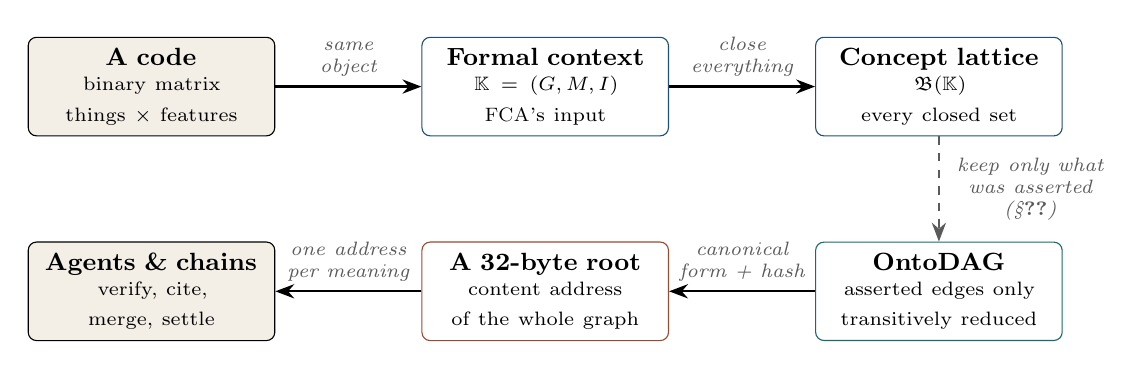
\begin{tikzpicture}[
  font=\small,
  box/.style={draw, rounded corners=3pt, minimum height=1.05cm,
              text width=2.85cm, align=center, inner sep=4pt},
  lbl/.style={font=\scriptsize\itshape, text=odgrey, align=center},
  ar/.style={-{Stealth[length=2.4mm]}, thick}]

\node[box, fill=odsand] (code) at (0,0)
  {\textbf{A code}\\[1pt]\scriptsize binary matrix\\\scriptsize
   things $\times$ features};
\node[box, fill=white, draw=odblue] (ctx) at (5.0,0)
  {\textbf{Formal context}\\[1pt]\scriptsize $\ctx=(G,M,I)$\\\scriptsize
   \fca{}'s input};
\node[box, fill=white, draw=odblue] (lat) at (10.0,0)
  {\textbf{Concept lattice}\\[1pt]\scriptsize $\Bcl(\ctx)$\\\scriptsize
   every closed set};
\node[box, fill=white, draw=odteal] (dag) at (10.0,-2.6)
  {\textbf{\odag{}}\\[1pt]\scriptsize asserted edges only\\\scriptsize
   transitively reduced};
\node[box, fill=white, draw=odrust] (root) at (5.0,-2.6)
  {\textbf{A 32-byte root}\\[1pt]\scriptsize content address\\\scriptsize
   of the whole graph};
\node[box, fill=odsand] (uses) at (0,-2.6)
  {\textbf{Agents \& chains}\\[1pt]\scriptsize verify, cite,\\\scriptsize
   merge, settle};

\draw[ar] (code) -- node[lbl, above]{same\\object} (ctx);
\draw[ar] (ctx)  -- node[lbl, above]{close\\everything} (lat);
\draw[ar, dashed, odgrey] (lat) -- node[lbl, right, xshift=1mm]
  {keep only what\\was asserted\\(\S\ref{sec:dictionary})} (dag);
\draw[ar] (dag)  -- node[lbl, above]{canonical\\form + hash} (root);
\draw[ar] (root) -- node[lbl, above]{one address\\per meaning} (uses);
\end{tikzpicture}
\caption{The road this paper travels. A neural code and a formal context are
the same mathematical object seen by two communities. Closing the context
gives the concept lattice, the object \fca{} studies. \odag{} sits below it:
the asserted fragment, kept in a unique minimal form, which is what allows the
whole graph to have a single content address --- and that address is what AI
agents and cryptographic systems actually want.}
\label{fig:roadmap}
\end{figure}

Figure~\ref{fig:roadmap} shows the route. We will walk it from left to right.

\subsection{Reproducibility}

Every quantitative claim in this paper --- concept counts, lattice sizes,
canonical root hashes, the round-trip between codes and graphs --- is computed
by \file{paper/experiments/fca_experiments.py}, which uses only the Python
standard library plus \odag{} itself. Its full output is reproduced in
Appendix~\ref{sec:experiments}, and the figures drawn from data are generated
from the same run. Where a number appears in the text it is marked with a
box like this one:

\begin{measured}
Running example: 6 documents $\times$ 5 properties, $57\%$ of cells filled.
\fca{} finds \textbf{10} formal concepts (out of $2^5=32$ conceivable
property sets). The same facts as an \odag{}: \textbf{11} nodes and
\textbf{17} asserted edges.
\end{measured}

\section{The mathematics you need (and no more)}
\label{sec:orders}

This section builds, from scratch, the handful of ideas both formalisms rest
on. If you know what a lattice and a transitive reduction are, skim to
Section~\ref{sec:transitive-reduction} for the uniqueness theorem, which is
the load-bearing fact of the whole paper, and then move on.

\subsection{Sets, and the one relation that matters}

A \emph{set} is a collection of distinct things, written with braces:
$\{a, b, c\}$. Two operations will appear on every page:

\begin{itemize}[leftmargin=1.4em]
\item \textbf{Intersection} $A \cap B$: the things in \emph{both} $A$ and $B$.
\item \textbf{Union} $A \cup B$: the things in \emph{either}.
\end{itemize}

And one relation, which is the real subject of this paper:

\begin{itemize}[leftmargin=1.4em]
\item \textbf{Containment} $A \subseteq B$: every element of $A$ is also an
  element of $B$. We say $A$ is a \emph{subset} of $B$. If additionally
  $A \neq B$ we write $A \subsetneq B$ and say \emph{strict} subset.
\end{itemize}

Containment is the prototype of everything that follows. When we say
``a spaniel is a dog'', ``\texttt{outbound.pdf} is a Japan document'', or
``$3\,\mathrm{kg}$ is within $0$--$5\,\mathrm{kg}$'', we are making a
statement with the same shape: one thing is a special case of another. In
every formalism in this paper that statement will turn out to be, literally,
a containment of sets --- of properties, of members, or of numerical values.

\subsection{Partial orders}

\begin{definition}[Partial order]
A \emph{partial order} on a set $P$ is a relation $\leq$ satisfying, for all
$x, y, z \in P$:
\begin{enumerate}[label=(\roman*),leftmargin=2.2em]
\item \textbf{reflexivity}: $x \leq x$;
\item \textbf{antisymmetry}: if $x \leq y$ and $y \leq x$ then $x = y$;
\item \textbf{transitivity}: if $x \leq y$ and $y \leq z$ then $x \leq z$.
\end{enumerate}
The pair $(P, \leq)$ is a \emph{partially ordered set}, or \emph{poset}.
\end{definition}

The word ``partial'' is the important one. In a \emph{total} order --- like
the numbers on a ruler --- any two elements are comparable: given $x$ and $y$,
either $x \leq y$ or $y \leq x$. In a partial order they need not be.
\textsf{Flight} and \textsf{Hotel} are simply incomparable: neither is a
special case of the other. This is not a defect of the model; it is the whole
point. Reality is full of incomparable things, and any structure that forces a
comparison (a filing cabinet, a folder tree, an alphabetical list) is lying
about something.

\begin{example}
Containment on sets is a partial order. $\{a\} \subseteq \{a,b\}$, and
$\{a\}$ and $\{b\}$ are incomparable. Divisibility on the positive integers is
another: $3 \leq 12$ because $3$ divides $12$; $3$ and $5$ are incomparable.
Hold on to the divisibility example --- Leibniz built an entire scheme of
conceptual notation on it (Section~\ref{sec:leibniz-note}).
\end{example}

\subsection{Drawing a poset: Hasse diagrams}

Drawing every arrow of a partial order is hopeless: transitivity means a chain
of length $n$ needs $\binom{n}{2}$ arrows, almost all of them redundant. The
standard solution is to draw only the arrows you cannot infer.

\begin{definition}[Cover]
In a poset, $y$ \emph{covers} $x$ (written $x \lessdot y$) when $x < y$ and
there is no $z$ with $x < z < y$: nothing sits strictly between them.
\end{definition}

\begin{definition}[Hasse diagram]
The \emph{Hasse diagram} of a finite poset draws one node per element and one
line per covering pair, with the greater element placed higher. All other
relationships are read off by following lines upward.
\end{definition}

\begin{figure}[t]
\centering
\begin{subfigure}[b]{0.46\textwidth}\centering
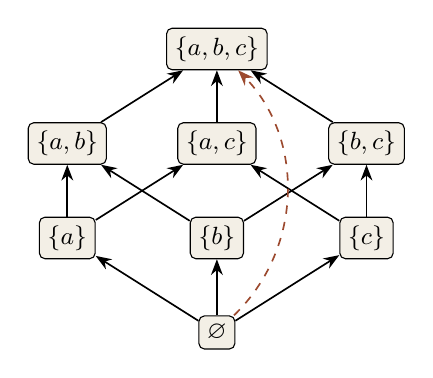
\begin{tikzpicture}[font=\small, node distance=1.05cm,
  n/.style={draw, rounded corners=2pt, inner sep=3pt, fill=odsand},
  e/.style={-{Stealth[length=2mm]}, semithick},
  r/.style={-{Stealth[length=2mm]}, semithick, odrust, dashed}]
\node[n] (abc) at (0,2.4) {$\{a,b,c\}$};
\node[n] (ab) at (-1.9,1.2) {$\{a,b\}$};
\node[n] (ac) at (0,1.2) {$\{a,c\}$};
\node[n] (bc) at (1.9,1.2) {$\{b,c\}$};
\node[n] (a) at (-1.9,0) {$\{a\}$};
\node[n] (b) at (0,0) {$\{b\}$};
\node[n] (c) at (1.9,0) {$\{c\}$};
\node[n] (e) at (0,-1.2) {$\varnothing$};
\foreach \x/\y in {a/ab,a/ac,b/ab,b/bc,c/ac,c/bc,ab/abc,ac/abc,bc/abc,
                   e/a,e/b,e/c}
  \draw[e] (\x) -- (\y);
\draw[r, bend right=45] (e) to (abc);
\end{tikzpicture}
\caption{All subsets of $\{a,b,c\}$ ordered by $\subseteq$. Solid arrows are
covers; the dashed one is an example of the many relationships a Hasse
diagram leaves implicit ($\varnothing \subseteq \{a,b,c\}$, readable by
walking up).}
\end{subfigure}\hfill
\begin{subfigure}[b]{0.46\textwidth}\centering
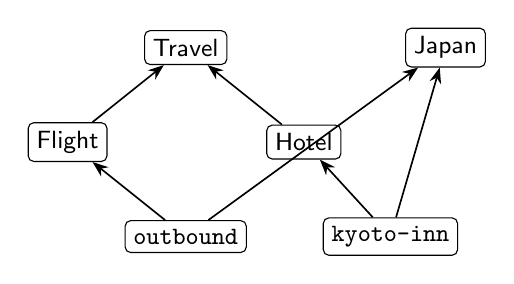
\begin{tikzpicture}[font=\small,
  n/.style={draw, rounded corners=2pt, inner sep=3pt, fill=white},
  e/.style={-{Stealth[length=2mm]}, semithick}]
\node[n] (t) at (0,2.4) {\textsf{Travel}};
\node[n] (f) at (-1.5,1.2) {\textsf{Flight}};
\node[n] (h) at (1.5,1.2) {\textsf{Hotel}};
\node[n] (j) at (3.3,2.4) {\textsf{Japan}};
\node[n] (o) at (0,0) {\texttt{outbound}};
\node[n] (k) at (2.6,0) {\texttt{kyoto-inn}};
\draw[e] (f) -- (t); \draw[e] (h) -- (t);
\draw[e] (o) -- (f); \draw[e] (o) -- (j);
\draw[e] (k) -- (h); \draw[e] (k) -- (j);
\end{tikzpicture}
\vspace{6mm}
\caption{Part of the running example. \texttt{outbound} has two parents; it
is a flight \emph{and} a Japan document. No tree can draw this.}
\end{subfigure}
\caption{Hasse diagrams. Higher means more general.}
\label{fig:hasse}
\end{figure}

A Hasse diagram is an act of compression: it stores the minimum and recovers
the rest by walking. \odag{} does the same thing with its actual storage, and
Section~\ref{sec:transitive-reduction} is about why that is safe.

\subsection{Directed graphs, reachability, cycles}

A \emph{directed graph} (digraph) is a set of nodes plus a set of arrows
(\emph{edges}) between them. Unlike a poset, a digraph carries no promise of
transitivity or antisymmetry --- it is just arrows.

\begin{definition}[Reachability]
Node $y$ is \emph{reachable} from $x$ if there is a path
$x \to \cdots \to y$ following arrows forwards. Every node is reachable from
itself by the empty path.
\end{definition}

\begin{definition}[DAG]
A \emph{directed acyclic graph} (DAG) is a digraph with no cycles: you can
never leave a node and return to it.
\end{definition}

The connection to posets is the reason DAGs matter here:

\begin{proposition}
\label{prop:dag-poset}
Reachability in a DAG is a partial order. Conversely, every finite poset is
the reachability order of a DAG --- for instance, of its Hasse diagram.
\end{proposition}

\noindent Reflexivity holds by the empty path, transitivity by concatenating
paths, and antisymmetry is exactly acyclicity: if $y$ were reachable from $x$
and $x$ from $y$ with $x \neq y$, the concatenation would be a cycle. So
\textbf{a DAG is a poset you can store}, and the acyclicity check that
\odag{} performs on every write (\S\ref{sec:put}) is the mechanism that keeps
the stored object a legitimate partial order.

\begin{definition}[Cone]
For a node $x$ in a DAG, its \emph{descendant cone} $\cone{x}$ is the set of
nodes reachable from $x$, including $x$ itself. Its \emph{ancestor cone}
$\up{x}$ is the set of nodes from which $x$ is reachable, again including $x$.
\end{definition}

We draw more general things higher and let edges point upward, from special to
general. So $\up{x}$ --- everything $x$ is a special case of --- is above $x$,
and $\cone{x}$ --- everything that is a special case of $x$ --- is below.
The cone is the single most important object in this paper. In \odag{} it is
the answer to a one-word query, in \fca{} it is a concept's extent, and in a
neural code it is the set of stimuli that activate a given unit.

\subsection{Transitive closure and transitive reduction}
\label{sec:transitive-reduction}

Two operations turn one digraph into another.

\begin{definition}[Transitive closure]
The \emph{transitive closure} $G^{+}$ of a digraph $G$ has the same nodes and
an edge $x \to y$ whenever $y$ is reachable from $x$ in $G$. It adds every
shortcut.
\end{definition}

\begin{definition}[Transitive reduction]
A \emph{transitive reduction} of $G$ is a digraph $\reduc{G}$ with the same
nodes and the same reachability, having as few edges as possible. It removes
every shortcut.
\end{definition}

Closure and reduction are opposite ends of a family of graphs that all say the
same thing. And now the fact that everything in \odag{} hangs from:

\begin{theorem}[Uniqueness of the reduction; \citealp{aho1972}]
\label{thm:unique-reduction}
For a finite DAG, the transitive reduction exists, is unique, and is a
subgraph of the original. It consists of exactly the covering pairs of the
reachability order --- i.e.\ it is the Hasse diagram.
\end{theorem}

\begin{proof}[Why it is true, informally]
Call an edge $x \to y$ \emph{redundant} if $y$ is reachable from $x$ by some
\emph{other} path. In a DAG a redundant edge can always be deleted without
changing reachability, because the alternative path survives the deletion ---
that path cannot pass through the edge $x \to y$ itself, since doing so would
require returning to $x$, which acyclicity forbids. So deleting redundant
edges one at a time terminates, and it terminates at the set of non-redundant
edges, which is determined by the reachability relation alone. Determined
means unique: the order of deletion cannot matter.

The caveat is worth stating, because it explains why the theorem is about
\emph{acyclic} graphs. In a graph with a cycle $x \to y \to x$, both edges are
redundant given the other, and you may delete either but not both --- so there
are two equally minimal answers and no canonical one.
\end{proof}

\begin{keyidea}
\textbf{Uniqueness is the seed of everything.} Because the reduction is
unique, a category structure has exactly \emph{one} minimal representation.
Two people who know the same things, having built their graphs in different
orders and having typed some redundant links along the way, end up with the
byte-identical graph. That is what lets \odag{} give the whole structure a
single fingerprint (\S\ref{sec:canonical}), and it is why the same knowledge
has the same address on a content-addressed network
(\S\ref{sec:crypto}).
\end{keyidea}

\begin{figure}[t]
\centering
\begin{subfigure}[b]{0.48\textwidth}\centering
  \dotfig[0.95]{reduction_before}
  \caption{As typed: someone asserted the dashed edge as well.}
\end{subfigure}\hfill
\begin{subfigure}[b]{0.48\textwidth}\centering
  \dotfig[0.95]{reduction_after}
  \caption{As stored: the shortcut is dropped. Reachability is unchanged.}
\end{subfigure}
\caption{Transitive reduction in action. \texttt{boarding-pass} is still under
\textsf{Japan} --- via \texttt{outbound.pdf} --- so storing the direct edge
would add nothing but would make the stored form depend on what the user
happened to type. (Figures generated with Graphviz and converted by
\texttt{dot2tex}; see Appendix~\ref{sec:colophon}.)}
\label{fig:reduction}
\end{figure}

\subsection{Lattices: when meets and joins always exist}

Posets can be missing things. In Figure~\ref{fig:hasse}(b), what is the most
specific thing that is both a \textsf{Flight} and a \textsf{Japan} document?
Looking at the picture, \texttt{outbound} is \emph{a} thing below both --- but
is it \emph{the} most specific such thing? If we later add another flight to
Japan, there will be two incomparable things below both, and no single
best answer. The poset has a gap where an answer ought to be.

\begin{definition}[Meet and join]
Let $x, y$ be elements of a poset. A \emph{lower bound} of $\{x,y\}$ is any
$z$ with $z \leq x$ and $z \leq y$. If among all lower bounds there is a
greatest one, it is called the \emph{meet}, written $x \wedge y$. Dually, the
least upper bound, if it exists, is the \emph{join} $x \vee y$.
\end{definition}

\begin{definition}[Lattice, complete lattice]
A poset is a \emph{lattice} if every pair of elements has both a meet and a
join. It is a \emph{complete lattice} if \emph{every} subset --- including the
empty set and infinite subsets --- has a meet and a join. A complete lattice
automatically has a greatest element $\top$ and a least element $\bot$.
\end{definition}

\begin{example}
The subsets of $\{a,b,c\}$ (Figure~\ref{fig:hasse}(a)) form a complete
lattice: meet is $\cap$, join is $\cup$, $\top = \{a,b,c\}$,
$\bot = \varnothing$. This is the model to keep in mind: \textbf{a lattice is
a system of sets closed under intersection}, dressed up.
\end{example}

The lattice property is a strong demand. It says that for \emph{any} question
of the form ``what is the most specific concept covering both of these?''
there is a unique answer already in the structure. \fca{}'s central theorem
guarantees exactly that (\S\ref{sec:basic-theorem}) --- and paying for that
guarantee, in storage and in computation, is the main cost \odag{} declines
to pay (\S\ref{sec:not-closed}).

\subsection{Closure operators, and the Galois connection}
\label{sec:closure}

One more piece of machinery, because it is how \fca{} actually works.

\begin{definition}[Closure operator]
A map $c$ from subsets of a set $S$ to subsets of $S$ is a \emph{closure
operator} if for all $A, B \subseteq S$:
\begin{enumerate}[label=(\roman*),leftmargin=2.2em]
\item \textbf{extensive}: $A \subseteq c(A)$ --- closing only adds;
\item \textbf{monotone}: $A \subseteq B \implies c(A) \subseteq c(B)$ ---
  more input, more output;
\item \textbf{idempotent}: $c(c(A)) = c(A)$ --- closing twice is closing once.
\end{enumerate}
A set with $c(A) = A$ is called \emph{closed}.
\end{definition}

\begin{example}
On a DAG, ``take the ancestor cone of everything in $A$'' is a closure
operator: it only adds nodes, it respects containment, and doing it twice
finds nothing new because ancestry is transitive. We will meet this operator
again in Section~\ref{sec:dictionary}, where it turns out to be the
\odag{} analogue of \fca{}'s closure.
\end{example}

\begin{proposition}
\label{prop:closed-sets-lattice}
The closed sets of a closure operator on $S$, ordered by $\subseteq$, form a
complete lattice. The meet of a family of closed sets is their intersection;
the join is the closure of their union.
\end{proposition}

This is why lattices keep appearing: any time you have a notion of ``close
this set up under some rule'', the closed sets are automatically a complete
lattice. \fca{} is, at bottom, the study of one particular closure operator.

\begin{definition}[Galois connection]
Given two sets $X$ and $Y$, a pair of maps
$f: \mathcal{P}(X) \to \mathcal{P}(Y)$ and
$g: \mathcal{P}(Y) \to \mathcal{P}(X)$ forms a \emph{(antitone) Galois
connection} when
\[
  A \subseteq g(B) \iff B \subseteq f(A)
  \qquad\text{for all } A \subseteq X,\ B \subseteq Y .
\]
Both maps reverse containment ($A \subseteq A' \implies f(A') \subseteq
f(A)$), and both composites $g \circ f$ and $f \circ g$ are closure operators.
\end{definition}

The containment reversal is intuitive once seen in an example: the more
properties you demand, the fewer things satisfy them; the more things you must
cover, the fewer properties they all share. That trade-off \emph{is} the
Galois connection, and Section~\ref{sec:derivation} makes it concrete.

\begin{exercise}
Check that ``the set of neurons active for every stimulus in $A$'' and ``the
set of stimuli that activate every neuron in $B$'' form a Galois connection
between stimuli and neurons. You have just derived \fca{} from the neural code
picture --- which is the content of Section~\ref{sec:code-is-context}.
\end{exercise}

\begin{remark}[Further reading]
The standard undergraduate text on this material is
\citet{davey2002}; \citet{birkhoff1940} is the classical source. Everything
above is in their first two chapters.
\end{remark}

\subsection{Summary of Section~\ref{sec:orders}}

\begin{center}
\small
\begin{tabularx}{\textwidth}{lX}
\toprule
\textbf{Idea} & \textbf{Why it appears later}\\
\midrule
Containment $\subseteq$ & the single shape of every ``is-a'' claim\\
Partial order & incomparable things are allowed; trees forbid them\\
DAG & a poset you can store; acyclicity $=$ antisymmetry\\
Cone $\cone{x}$ & \odag{}'s query answer; \fca{}'s extent; a code's stimulus set\\
Transitive reduction & unique (Thm~\ref{thm:unique-reduction}) $\Rightarrow$ canonical form $\Rightarrow$ one hash\\
Lattice & every pair has a meet: \fca{} guarantees it, \odag{} declines to\\
Closure operator & closed sets always form a lattice (Prop.~\ref{prop:closed-sets-lattice})\\
Galois connection & the exact machine that turns a binary table into concepts\\
\bottomrule
\end{tabularx}
\end{center}

\section{Where the idea came from: codes in the brain}
\label{sec:neural}

This section is the origin story. It is not a prerequisite for the technical
content --- a reader in a hurry can skip to Section~\ref{sec:fca} --- but it
explains \emph{why} anyone would build a system like \odag{} in the first
place, and it contains the observation that the rest of the paper formalises.

\subsection{What a neural code is}

A sensory neuron does not report a number to a central reader. It fires, or it
does not, and what it means is determined entirely by which things in the
world make it fire. Record from many neurons at once while showing many
stimuli, threshold each response into ``active'' or ``silent'', and you have a
matrix:

\begin{center}
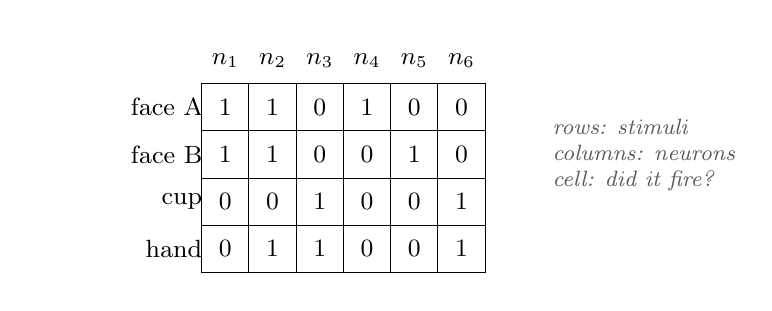
\begin{tikzpicture}[font=\small]
\matrix (m) [matrix of nodes, nodes={draw, minimum size=6mm, anchor=center,
             inner sep=0pt, font=\small}, column sep=-\pgflinewidth,
             row sep=-\pgflinewidth,
             row 1/.style={nodes={draw=none, fill=none}},
             column 1/.style={nodes={draw=none, fill=none, text width=2.1cm,
                              align=right}}]
{
              & $n_1$ & $n_2$ & $n_3$ & $n_4$ & $n_5$ & $n_6$ \\
  face A      & 1     & 1     & 0     & 1     & 0     & 0     \\
  face B      & 1     & 1     & 0     & 0     & 1     & 0     \\
  cup         & 0     & 0     & 1     & 0     & 0     & 1     \\
  hand        & 0     & 1     & 1     & 0     & 0     & 1     \\
};
\node[font=\footnotesize\itshape, text=odgrey, anchor=west, align=left]
  at ([xshift=6mm]m.east)
  {rows: stimuli\\columns: neurons\\cell: did it fire?};
\end{tikzpicture}
\end{center}

\noindent
Real cortical codes of this kind are \emph{sparse}: for any one stimulus only
a small fraction of the units are active \citep{barlow1972,foldiak1990,%
olshausen1996}. Sparseness is not an accident of measurement. It is what you
get if you ask a network to represent its input economically --- to spend few
active units per item while keeping items distinguishable --- and it is the
representational regime in which the observation below has teeth.

Between two extremes:

\begin{itemize}[leftmargin=1.4em]
\item A \textbf{localist} code gives each thing its own unit --- the
  ``grandmother cell''. Simple to read, but you need as many units as things,
  and nothing is shared between related items.
\item A \textbf{dense distributed} code has roughly half the units active for
  everything. Maximally efficient in bits, but the representation of one item
  overlaps every other for no meaningful reason.
\item A \textbf{sparse} code sits between: each item activates a small set,
  and --- crucially --- \emph{related items activate overlapping sets}.
\end{itemize}

That last clause is where structure appears.

\subsection{The observation}

Take the code for ``spaniel'' and the code for ``dog''. In a sparse code that
has learned anything about the world, the units active for a spaniel will
include the units that respond to dogs in general, plus some extra ones
specific to spaniels. Write $\code{x}$ for the set of active units of
stimulus $x$. Then
\[
  \code{\text{dog}} \;\subseteq\; \code{\text{spaniel}} .
\]

Read that line slowly, because it is the whole idea. The taxonomic statement
``a spaniel is a dog'' has become a containment between two sets of active
units. \textbf{More specific means more bits on.} And containment brings its
entire order theory (Section~\ref{sec:orders}) along with it: the codes are
partially ordered by $\subseteq$, incomparable things are exactly things
neither of which is a special case of the other, and the covering relation of
that order is a Hasse diagram --- a category graph.

\begin{keyidea}
\textbf{The category graph need not be stored anywhere.} No synapse has to
encode the arrow from spaniel to dog. The arrow is a \emph{consequence} of
which units overlap. Associations between concepts can be implicit in the
code rather than carried by connections \citep{foldiak2003}.
\end{keyidea}

This has three immediate consequences that shaped \odag{}'s design, and each
of them will reappear later in the paper wearing engineering clothes.

\begin{enumerate}[leftmargin=1.6em]
\item \textbf{Queries are set operations.} ``Find everything that is both a
  dog and brown'' becomes: find every $x$ whose code contains the dog units
  \emph{and} the brown units. A conjunctive query is an intersection --- or,
  in hardware terms, a bitwise \textsc{and}. This is \odag{}'s only query
  primitive (\S\ref{sec:get}).
\item \textbf{Similarity is overlap.} Two items with largely overlapping codes
  are similar without anyone having said so. Graded retrieval --- ``what is
  most like this?'' --- is $|\code{x} \cap \code{y}|$, computed on the same
  representation as exact retrieval, with a threshold as the only difference
  \citep{foldiak2003}.
\item \textbf{Generalisation is a subset.} A concept more general than $x$ is
  a \emph{subset} of $x$'s code. Dropping bits is abstracting. This is why
  Borges's Funes, who remembered every instant in full detail and could
  therefore drop nothing, was ``virtually incapable of general, platonic
  ideas'' \citep{borges1942}: no compression, no concepts.
\end{enumerate}

\subsection{The code matrix is a formal context}
\label{sec:code-is-context}

Here is the bridge, stated plainly. Everything in
Section~\ref{sec:fca} is a development of this single sentence:

\begin{keyidea}
A binary stimulus $\times$ neuron matrix and a \emph{formal context}
$\ctx = (G, M, I)$ are the same object. Objects $G$ are the stimuli,
attributes $M$ are the neurons, and the incidence $I$ says ``this neuron fired
for this stimulus''. Everything \fca{} proves about formal contexts is
therefore a theorem about neural codes.
\end{keyidea}

This is not a metaphor invented for this paper; it is a published research
programme. \citet{endres2008} applied \fca{} to recordings from macaque
superior temporal sulcus, building the formal context from spike counts by an
exact Bayesian thresholding procedure and then reading the concept lattice as
a description of what the neural population represents. The lattice exposed a
hierarchical organisation of face representations and evidence for a
product-of-experts style code --- structure that is invisible in the raw
firing rates and that no dimensionality reduction into a Euclidean space would
have expressed, because the structure is \emph{ordinal}, not metric. The
follow-up \citep{endres2010} pushed the same machinery toward semantic
decoding.

\begin{figure}[t]
\centering
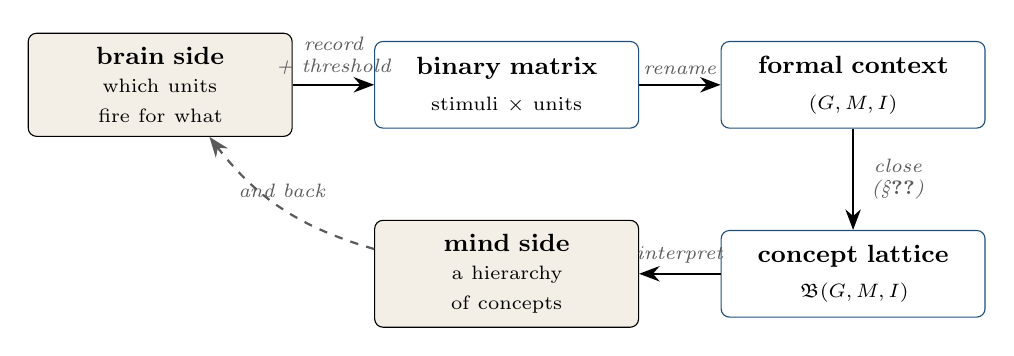
\begin{tikzpicture}[font=\small,
  b/.style={draw, rounded corners=3pt, align=center, inner sep=5pt,
            minimum height=1.1cm, text width=3.0cm},
  ar/.style={-{Stealth[length=2.6mm]}, thick},
  lab/.style={font=\scriptsize\itshape, text=odgrey, align=center}]

\node[b, fill=odsand] (brain) at (0,0)
  {\textbf{brain side}\\[2pt]\scriptsize which units\\\scriptsize fire for what};
\node[b, draw=odblue] (matrix) at (4.4,0)
  {\textbf{binary matrix}\\[2pt]\scriptsize stimuli $\times$ units};
\node[b, draw=odblue] (ctx) at (8.8,0)
  {\textbf{formal context}\\[2pt]\scriptsize $(G,M,I)$};
\node[b, fill=odsand] (mind) at (4.4,-2.4)
  {\textbf{mind side}\\[2pt]\scriptsize a hierarchy\\\scriptsize of concepts};
\node[b, draw=odblue] (lat) at (8.8,-2.4)
  {\textbf{concept lattice}\\[2pt]\scriptsize $\Bcl(G,M,I)$};

\draw[ar] (brain) -- node[lab,above]{record\\+ threshold} (matrix);
\draw[ar] (matrix) -- node[lab,above]{rename} (ctx);
\draw[ar] (ctx) -- node[lab,right,xshift=1mm]{close\\(\S\ref{sec:derivation})} (lat);
\draw[ar] (lat) -- node[lab,above]{interpret} (mind);
\draw[ar, dashed, odgrey] (mind) to[bend left=18]
  node[lab,above]{and back} (brain);
\end{tikzpicture}
\caption{The mind--brain round trip that motivates the whole exercise. The
left column is neuroscience, the right column is mathematics, and the two
middle arrows are pure renaming. Because the maps in
Section~\ref{sec:derivation} are invertible, the trip can be made in either
direction: a code determines a concept hierarchy, and a concept hierarchy can
be embedded into a code.}
\label{fig:mind-brain}
\end{figure}

\subsection{Why this is more than a curiosity}

Two directions of travel, both useful.

\paragraph{Code $\to$ concepts (interpretation).} Given a recorded population
code, the concept lattice tells you what the population distinguishes and how
its distinctions nest. This is a tool for neuroscience, and it has the
attractive property of being \emph{non-parametric about geometry}: it assumes
nothing about distances, only about which units fire.

\paragraph{Concepts $\to$ code (design).} Given an ontology you want a system
to hold, you can embed it in a binary code such that subsumption is subset
containment. This is the direction \odag{} cares about, and
Section~\ref{sec:dictionary} shows it is exact: the reflexive ancestor set of
each node \emph{is} such a code, and the graph can be reconstructed from the
codes with nothing lost. Historically the same idea has been rediscovered
several times: as bitvector encodings of type lattices for fast subsumption
checks in programming languages \citep{aitkaci1989}; as faceted
classification in library science, where \citet{ranganathan1933} proposed
describing a work by a \emph{set} of independent facets rather than one
shelf path --- the librarians' independent discovery that the lattice, not
the tree, is the honest shape; as sparse distributed
representations and hyperdimensional computing
\citep{kanerva2009,plate1995}; and, three centuries earlier, as Leibniz's
prime-number notation.

\subsection{A note on Leibniz}
\label{sec:leibniz-note}

Leibniz's scheme deserves a paragraph, because it is the same lattice written
in a different alphabet and it makes the algebra vivid \citep{leibniz1666}.
Assign a distinct prime to each primitive concept, and give a composite
concept the \emph{product} of its constituents' primes. If
$\textsf{animal} = 2$ and $\textsf{rational} = 3$, then $\textsf{human} = 6$.
Now:
\[
  A \text{ subsumes } B \iff \text{the number of } A \text{ divides the number
  of } B .
\]
Divisibility of square-free numbers is exactly set containment on the sets of
prime factors. So Leibniz's ``let us calculate'' and the bitwise-\textsc{and}
of two cone bitmaps are the same operation in different notation, three and a
half centuries apart. What Leibniz lacked was not the algebra but a
\emph{source} for the primitives; \fca{} supplies one (derive them from data),
and \odag{} supplies another (let people assert them, and merge what they
assert).

\subsection{Why not just use vectors?}

A reader who has met machine learning will ask why one would use sets of bits
rather than real-valued embeddings, which are what modern systems actually
use. The honest answer is that they solve different problems, and the
difference is the theme of this paper.

\begin{center}
\small
\begin{tabularx}{\textwidth}{@{}lXX@{}}
\toprule
 & \textbf{Sparse binary code / DAG} & \textbf{Dense real embedding}\\
\midrule
Subsumption & exact set containment, decidable & approximate, thresholded\\
Similarity  & overlap count, exact & cosine distance, learned\\
Query       & intersection: complete and sound & nearest neighbours: neither\\
Novel item  & new bit, no retraining & re-embed, possibly retrain\\
Explanation & the shared bits \emph{are} the reason & post-hoc at best\\
Identity    & a name; stable & a vector; changes when the model does\\
Merging two & union of assertions, converges & incomparable spaces\\
\bottomrule
\end{tabularx}
\end{center}

Embeddings are superb at recall from vague input, which is precisely what an
exact structure cannot do. Discrete structures are superb at exactness,
verifiability and merging, which is precisely what an embedding cannot do.
Section~\ref{sec:agents} argues that a practical agent memory wants both, with
the embedding proposing and the DAG disposing --- and that the interesting
engineering is in the interface between them, not in a winner.

\begin{tryit}
Take the four-stimulus code at the start of this section. Which stimuli
activate a superset of $\{n_2, n_3\}$? (Answer: only \emph{hand}.) Which pairs
of stimuli have overlapping codes? Sketch the containment order on the four
codewords --- you will find that \emph{face A} and \emph{face B} are
incomparable, sharing $\{n_1, n_2\}$, which is the code of a concept that has
no name in the table but plainly ought to. That nameless shared concept is a
formal concept, and finding all of them is what Section~\ref{sec:fca} is
about.
\end{tryit}

\section{Formal Concept Analysis from scratch}
\label{sec:fca}

\fca{} was introduced by \citet{wille1982} as a way of ``restructuring lattice
theory'' --- taking an abstract branch of algebra and giving it a concrete
interpretation in terms of objects, attributes and concepts, so that lattice
diagrams become something a domain expert can read. The standard reference is
\citet{ganter1999}; \citet{carpineto2004} and \citet{priss2006} are gentler
surveys.

This section develops the theory on the running example of
Section~\ref{sec:running-example}. Everything is computed rather than
asserted: the numbers come from \file{fca_experiments.py}
(Appendix~\ref{sec:experiments}).

\subsection{The formal context}

\begin{definition}[Formal context]
A \emph{formal context} is a triple $\ctx = (G, M, I)$ where $G$ is a set of
\emph{objects}, $M$ is a set of \emph{attributes}, and
$I \subseteq G \times M$ is an \emph{incidence relation}. We write $g\,I\,m$
for ``object $g$ has attribute $m$''.
\end{definition}

The letters are from the German: \emph{Gegenst\"ande} (objects),
\emph{Merkmale} (attributes). A context is just a cross table, and our running
example is this one:

\begin{table}[h]
\centering
\small
\caption{The running example as a formal context $\ctx = (G, M, I)$: six
documents, five properties, $57\%$ of the cells filled.}
\label{tab:context}
\vspace{2mm}
\begin{tabular}{l ccccc}
\toprule
& \rotatebox{60}{\textsf{Flight}} & \rotatebox{60}{\textsf{Hotel}}
& \rotatebox{60}{\textsf{Japan}} & \rotatebox{60}{\textsf{Booked}}
& \rotatebox{60}{\textsf{Refundable}}\\
\midrule
\texttt{outbound.pdf}  & $\times$ &          & $\times$ & $\times$ & $\times$\\
\texttt{inbound.pdf}   & $\times$ &          & $\times$ & $\times$ &         \\
\texttt{kyoto-inn.pdf} &          & $\times$ & $\times$ & $\times$ & $\times$\\
\texttt{rail-pass.pdf} &          &          & $\times$ & $\times$ & $\times$\\
\texttt{paris-hop.pdf} & $\times$ &          &          & $\times$ &         \\
\texttt{visa-note.md}  &          &          & $\times$ &          &         \\
\bottomrule
\end{tabular}
\end{table}

Note what a context does \emph{not} contain. There is no hierarchy in it --- no
statement that \textsf{Flight} is a kind of anything, no statement that
\texttt{outbound.pdf} is more specific than \texttt{inbound.pdf}. The context
is raw co-occurrence. Everything hierarchical that follows will be
\emph{derived} from it. That is \fca{}'s central promise and, as we shall see,
also its central cost.

\subsection{The derivation operators}
\label{sec:derivation}

\begin{definition}[Derivation]
For a set of objects $A \subseteq G$ and a set of attributes $B \subseteq M$:
\[
  A' \;=\; \{\, m \in M \;:\; g\,I\,m \text{ for all } g \in A \,\},
  \qquad
  B' \;=\; \{\, g \in G \;:\; g\,I\,m \text{ for all } m \in B \,\}.
\]
$A'$ is ``the attributes shared by all of $A$''; $B'$ is ``the objects having
all of $B$''. Both are written with the same prime, and which one is meant is
determined by the argument.
\end{definition}

\begin{example}
In Table~\ref{tab:context}:
\begin{align*}
\{\texttt{outbound.pdf}, \texttt{inbound.pdf}\}' &=
  \{\textsf{Flight}, \textsf{Japan}, \textsf{Booked}\},\\
\{\textsf{Flight}, \textsf{Japan}\}' &=
  \{\texttt{outbound.pdf}, \texttt{inbound.pdf}\},\\
\{\textsf{Hotel}\}' &= \{\texttt{kyoto-inn.pdf}\}, \\
\varnothing' &= M \quad\text{(everything is shared by no objects at all).}
\end{align*}
\end{example}

The two maps form an (antitone) Galois connection in the sense of
Section~\ref{sec:closure}: enlarging $A$ can only shrink $A'$, and
$A \subseteq B' \iff B \subseteq A'$. Both composites are closure operators.
We write $A'' = (A')'$ and call it the closure of $A$.

\begin{pitfall}
The prime is not an inverse. $A''$ generally contains more than $A$: it is
$A$ plus every other object that happens to share all of $A$'s common
attributes. Try $A = \{\texttt{outbound.pdf}\}$: $A' =
\{\textsf{Flight},\textsf{Japan},\textsf{Booked},\textsf{Refundable}\}$ and
$A'' = \{\texttt{outbound.pdf}\}$ again --- but
$A = \{\texttt{visa-note.md}\}$ closes to $A'' =
\{\texttt{outbound.pdf}, \texttt{inbound.pdf}, \texttt{kyoto-inn.pdf},
\texttt{rail-pass.pdf}, \texttt{visa-note.md}\}$, because \texttt{visa-note}'s
only attribute is \textsf{Japan} and all those documents have it.
\end{pitfall}

\subsection{Formal concepts}

\begin{definition}[Formal concept]
A \emph{formal concept} of $\ctx$ is a pair $(A, B)$ with $A \subseteq G$,
$B \subseteq M$, $A' = B$ and $B' = A$. $A$ is the \emph{extent} (the things
falling under the concept), $B$ the \emph{intent} (the properties defining
it).
\end{definition}

The two conditions are a fixed-point demand, and they encode a very old
intuition about what a concept is: \emph{the extent and the intent must
determine each other exactly}. A concept is not any old pair of a set of
things and a set of properties. It is a pair in perfect balance: every object
in the extent has every attribute in the intent (that much is easy), and
crucially there is no object outside the extent that would also qualify, and
no attribute outside the intent that all the extent happens to share.

\begin{example}
$(\{\texttt{outbound.pdf}, \texttt{inbound.pdf}\},
\{\textsf{Flight}, \textsf{Japan}, \textsf{Booked}\})$ is a formal concept: the
two flights to Japan share exactly those three properties, and no other
document has all three. Informally, it is the concept \emph{Japanese flight
booking}, which nobody put in the table --- it emerged.

By contrast $(\{\texttt{outbound.pdf}\}, \{\textsf{Flight}\})$ is \emph{not} a
concept: \texttt{outbound.pdf} has more attributes than just \textsf{Flight},
so the pair is unbalanced.
\end{example}

\begin{proposition}
$(A,B)$ is a formal concept iff $A$ is a closed object set ($A''=A$) and
$B=A'$; equivalently iff $B$ is a closed attribute set ($B''=B$) and $A=B'$.
So concepts are in bijection with closed attribute sets, which is how
algorithms enumerate them.
\end{proposition}

\subsection{The concept lattice}
\label{sec:basic-theorem}

Order concepts by specificity: $(A_1, B_1) \leq (A_2, B_2)$ when
$A_1 \subseteq A_2$ --- equivalently, when $B_2 \subseteq B_1$. Fewer things,
more properties, further down. The set of all concepts under this order is
written $\Bcl(\ctx)$.

\begin{theorem}[Basic Theorem of \fca{}; \citealp{wille1982,ganter1999}]
\label{thm:basic}
$\Bcl(\ctx)$ is a complete lattice, in which
\[
  \bigwedge_{t \in T}(A_t, B_t) =
    \Bigl(\bigcap_{t} A_t,\ \bigl(\bigcup_{t} B_t\bigr)''\Bigr),
  \qquad
  \bigvee_{t \in T}(A_t, B_t) =
    \Bigl(\bigl(\bigcup_{t} A_t\bigr)'',\ \bigcap_{t} B_t\Bigr).
\]
Conversely, every complete lattice is isomorphic to the concept lattice of
some context. So ``complete lattice'' and ``concept lattice'' are the same
notion up to isomorphism.
\end{theorem}

Two things are worth extracting from that statement, one reassuring and one
expensive.

\emph{Reassuring:} meets are intersections of extents. ``The most specific
concept that is both a \textsf{Flight} and a \textsf{Japan} document'' always
exists, is unique, and is computed by intersecting. That is a strong
guarantee, and it is exactly what makes concept lattices navigable.

\emph{Expensive:} \emph{completeness} means \emph{every} subset has a meet,
including subsets nobody asked about. The lattice contains a concept for every
closed attribute set, whether or not any object realises it, whether or not
anybody would recognise it, and whether or not the co-occurrence that produced
it is a real regularity or a coincidence. Section~\ref{sec:explosion} measures
what that costs.

\subsection{Reading a line diagram}

\begin{figure}[t]
\centering
\dotfig[0.85]{lattice_travel}
\caption{The concept lattice of Table~\ref{tab:context}: 10 concepts, 13
covering edges, drawn with \fca{}'s standard \emph{reduced labelling}. Each
attribute and each object name appears exactly once. To read off whether an
object has an attribute, start at the object's node and walk \emph{upward}
along any lines: you have the attribute iff you can reach its label. The black
disc is a concept that introduces neither a new attribute nor a new object.
Diagram generated with Graphviz from the computed lattice.}
\label{fig:lattice}
\end{figure}

Figure~\ref{fig:lattice} shows the lattice. The convention deserves
explanation because it is initially surprising and then very economical.

In \emph{full labelling} you would write each concept's whole extent and whole
intent inside its node, which repeats every name many times. \emph{Reduced
labelling} writes each name once, at the concept where it is ``introduced'':

\begin{itemize}[leftmargin=1.4em]
\item attribute $m$ labels the concept $(m', m'')$ --- the \emph{largest}
  concept whose intent contains $m$;
\item object $g$ labels the concept $(g'', g')$ --- the \emph{smallest}
  concept whose extent contains $g$.
\end{itemize}

\noindent and then the reading rules recover everything:

\begin{itemize}[leftmargin=1.4em]
\item the \textbf{intent} of a concept is every attribute label reachable by
  walking \emph{up};
\item the \textbf{extent} is every object label reachable by walking
  \emph{down};
\item ``object $g$ has attribute $m$'' iff you can walk up from $g$'s label
  to $m$'s label.
\end{itemize}

\begin{tryit}
In Figure~\ref{fig:lattice}, find \texttt{rail-pass} and walk upward. You
should reach \textsf{Refundable}, \textsf{Japan} and \textsf{Booked}, but not
\textsf{Flight} or \textsf{Hotel}. Compare with Table~\ref{tab:context}. Then
find the concept where \textsf{Booked} sits and walk \emph{down}: you collect
all five booked documents --- and, satisfyingly, not \texttt{visa-note}.
\end{tryit}

\subsection{The full list, and what is in it}

Here is every concept of the running example, computed and sorted by extent
size. \texttt{Supp} is the extent size (in data-mining language, the support);
\texttt{stab} is Kuznetsov's \emph{stability} \citep{kuznetsov2007}, the
fraction of subsets of the extent that still close to the same intent --- a
measure of how much the concept depends on any particular object.

\begin{table}[h]
\centering\small
\caption{All 10 formal concepts of Table~\ref{tab:context}. Only 10 of the
$2^5 = 32$ conceivable attribute sets are closed.}
\label{tab:concepts}
\vspace{1mm}
\begin{tabular}{r l l r r}
\toprule
\# & \textbf{Intent} & \textbf{Extent} & supp & stab\\
\midrule
0 & $\varnothing$ & all six documents & 6 & 0.25\\
1 & \textsf{Booked} & all but \texttt{visa-note} & 5 & 0.38\\
2 & \textsf{Japan} & all but \texttt{paris-hop} & 5 & 0.50\\
3 & \textsf{Booked},\textsf{Japan} & \texttt{outbound},\texttt{inbound},\texttt{kyoto-inn},\texttt{rail-pass} & 4 & 0.38\\
4 & \textsf{Booked},\textsf{Flight} & \texttt{outbound},\texttt{inbound},\texttt{paris-hop} & 3 & 0.50\\
5 & \textsf{Booked},\textsf{Japan},\textsf{Refundable} & \texttt{outbound},\texttt{kyoto-inn},\texttt{rail-pass} & 3 & 0.62\\
6 & \textsf{Booked},\textsf{Flight},\textsf{Japan} & \texttt{outbound},\texttt{inbound} & 2 & 0.50\\
7 & \textsf{Booked},\textsf{Flight},\textsf{Japan},\textsf{Refundable} & \texttt{outbound} & 1 & 0.50\\
8 & \textsf{Booked},\textsf{Hotel},\textsf{Japan},\textsf{Refundable} & \texttt{kyoto-inn} & 1 & 0.50\\
9 & all five attributes & $\varnothing$ & 0 & 1.00\\
\bottomrule
\end{tabular}
\end{table}

Concepts 0 and 9 are the lattice's $\top$ and $\bot$: a complete lattice must
have them, so they are manufactured whether or not anything in the world
corresponds. Concept 9 is the concept of a document that is simultaneously a
flight and a hotel --- empty, and necessarily so. Concepts 3, 4, 5 and 6 are
the interesting ones: \emph{nobody wrote them down}, and each is a genuine
category (``booked Japan documents'', ``booked flights'', ``refundable Japan
bookings'', ``booked flights to Japan''). This is \fca{} doing what it is for.

\subsection{Implications}
\label{sec:implications}

\begin{definition}[Attribute implication]
For $B, C \subseteq M$, the implication $B \to C$ \emph{holds in} $\ctx$ if
every object having all attributes in $B$ also has all attributes in $C$;
equivalently, if $C \subseteq B''$.
\end{definition}

\begin{measured}
The single-premise implications of Table~\ref{tab:context}:
\[
\textsf{Flight} \to \textsf{Booked}, \qquad
\textsf{Refundable} \to \textsf{Booked}, \textsf{Japan}, \qquad
\textsf{Hotel} \to \textsf{Booked}, \textsf{Japan}, \textsf{Refundable}.
\]
\end{measured}

Read them aloud and the value is obvious: ``every flight here is booked'',
``everything refundable is a booked Japan document''. Read them again and the
danger is equally obvious: these are facts about \emph{this table}, not laws.
One unbooked flight destroys the first. Section~\ref{sec:learn-implications}
is about exactly this distinction, and it is the single most important thing
\odag{} must get right if it borrows anything from this part of \fca{}.

The set of all implications holding in a context is infinite (it is closed
under trivial consequences), but it has a canonical finite generating set:

\begin{theorem}[Duquenne--Guigues base; \citealp{guigues1986}]
Every formal context has a unique minimum-cardinality set of implications from
which all others follow, the \emph{stem base}. Its premises are the
\emph{pseudo-intents} of the context.
\end{theorem}

The stem base is a \emph{canonical} object: same context, same base. It is the
closest thing \fca{} has to \odag{}'s canonical form, and comparing the two
notions of canonicity (Section~\ref{sec:two-canonical-forms}) is one of the
more illuminating exercises in this paper.

\subsection{Computing: NextClosure and complexity}
\label{sec:algorithms}

The standard enumeration algorithm is \citeauthor{ganter1984}'s
\emph{NextClosure} \citeyearpar{ganter1984}. Fix an order on the attributes.
Every closed set has a successor in \emph{lectic} order (a variant of
alphabetical order on the characteristic bit vectors), computable directly.
Starting from $\varnothing''$ and repeatedly taking successors enumerates every
closed set, in order, using memory for one set at a time --- no lattice needs
to be held in RAM. The paper's implementation
(Appendix~\ref{sec:experiments}) is thirty lines and is checked against a
brute-force oracle on every example in this document.

Many faster algorithms exist --- Close-by-One and its descendants, Lindig's,
Titanic --- and they are compared empirically by \citet{kuznetsov2002} and
\citet{krajca2010}. None of them can escape the following.

\begin{theorem}[Hardness; \citealp{kuznetsov2001}]
The number of formal concepts of a context can be exponential in the size of
the context, and determining that number is $\#\mathrm{P}$-complete.
\end{theorem}

There is nothing pathological about the exponential case. It is reached by the
simplest imaginable table:

\begin{definition}[Contranominal scale]
$\mathbb{N}_n^c = (\{1,\dots,n\}, \{1,\dots,n\}, \neq)$: $n$ objects, $n$
attributes, and object $i$ has attribute $j$ exactly when $i \neq j$. Every
attribute subset is closed, so $|\Bcl| = 2^n$.
\end{definition}

\subsection{The explosion, measured}
\label{sec:explosion}

\begin{measured}
Contranominal scales, computed:

\smallskip
\centering\small
\begin{tabular}{rrrr}
\toprule
$n$ & concepts & \odag{} nodes & \odag{} edges\\
\midrule
 4 &      16 &  8 &  12\\
 8 &     256 & 16 &  56\\
10 &   1\,024 & 20 &  90\\
12 &   4\,096 & 24 & 132\\
\bottomrule
\end{tabular}
\end{measured}

\noindent
And on random data, where the effect is less extreme but still decisive.
Figure~\ref{fig:explosion} plots the mean number of concepts of a random
context with 30 objects and 12 attributes, against the number of crosses in
the table (which is what \odag{} would store as edges), as the density rises.

\begin{figure}[t]
\centering
\begin{tikzpicture}
\begin{axis}[
  width=0.78\textwidth, height=6.2cm,
  xlabel={density of the context (fraction of cells filled)},
  ylabel={count},
  xmin=0.05, xmax=0.65,
  legend pos=north west, legend cell align=left,
  grid=major, grid style={odgrey!20},
  every axis plot/.append style={very thick},
  tick label style={font=\small}, label style={font=\small},
  legend style={font=\small}]
\addplot[odrust, mark=*] table[x=density, y=concepts]
  {experiments/explosion.dat};
\addlegendentry{formal concepts (mean of 20)}
\addplot[odteal, mark=square*] table[x=density, y=edges]
  {experiments/explosion.dat};
\addlegendentry{crosses in the table $=$ \odag{} edges}
\end{axis}
\end{tikzpicture}
\caption{Random contexts, 30 objects $\times$ 12 attributes. The stored data
grows linearly with density; the concept lattice does not. At density $0.6$
the table has about 211 crosses and the lattice has about 550 concepts --- and
this is a \emph{small} context. Data from
\file{experiments/explosion.dat}, generated by the experiment script.}
\label{fig:explosion}
\end{figure}

This is not a criticism of \fca{}. Closing a context is an expensive
operation because \emph{the information is really there} --- those concepts
are genuinely supported by the data. It is, however, decisive for a system
that must hold a growing store in a browser tab, hash it after every edit, and
merge it with a stranger's copy. Section~\ref{sec:not-closed} returns to this.

\subsection{The parts of \fca{} beyond the basics}
\label{sec:fca-extensions}

\fca{} has grown a substantial toolbox in forty years. Six branches matter for
this paper; each reappears in Section~\ref{sec:learn} as a candidate for
adoption.

\paragraph{Many-valued contexts and conceptual scaling.} Real data has
numbers, not crosses. A \emph{many-valued context} $(G, M, W, I)$ assigns each
object a value in $W$ for each attribute; \emph{conceptual scaling} converts
it into an ordinary context by choosing, per attribute, a \emph{scale} that
says which comparisons matter \citep[ch.~1]{ganter1999}. The standard scales
are worth memorising because they are a checklist of ways to turn a value into
crosses:

\begin{center}\small
\begin{tabularx}{\textwidth}{@{}lXl@{}}
\toprule
\textbf{Scale} & \textbf{Turns a value into} & \textbf{Example}\\
\midrule
nominal      & one attribute per distinct value, mutually exclusive & colour\\
ordinal      & ``$\leq v$'' attributes, one per threshold & school grade\\
interordinal & both ``$\leq v$'' and ``$\geq v$'' & temperature ranges\\
biordinal    & two ordinal scales meeting in the middle & good/bad axes\\
contranominal& ``$\neq v$'' --- the exponential one & (avoid)\\
\bottomrule
\end{tabularx}
\end{center}

\paragraph{Pattern structures.} Scaling is lossy and arbitrary. Pattern
structures \citep{ganter2001} generalise \fca{} so that an object's
description need not be a set of attributes at all: it can be any element of a
meet-semilattice with a similarity operation $\sqcap$. The most-used instance
is the \emph{interval pattern structure}, where a description is an interval
and $\sqcap$ is the convex hull \citep{kaytoue2011}. Remember this; \odag{}'s
handling of typed values (\S\ref{sec:dimensions}) turns out to be an instance
of it that was arrived at independently.

\paragraph{Iceberg lattices and frequent closed itemsets.} Keep only concepts
whose extent exceeds a support threshold \citep{stumme2002}. The result is the
top of the lattice --- the ``iceberg'' --- and it is exactly the set of
frequent closed itemsets from association-rule mining \citep{pasquier1999}. A
principled way to be partial.

\paragraph{Stability.} A different filter: keep concepts that survive the
removal of objects \citep{kuznetsov2007}. Support asks ``how many?''; stability
asks ``how robust?''. The two disagree usefully, as
Table~\ref{tab:concepts} shows --- concept 5 has lower support than concept 3
but higher stability.

\paragraph{Boolean factor analysis.} \citet{belohlavek2010} proved that formal
concepts are exactly the optimal factors for exact Boolean matrix
decomposition: to write a binary matrix as a product of two binary matrices
with as few inner dimensions as possible, use concepts. This is the result
that connects \fca{} to the compression-based learning of
Section~\ref{sec:learn-mdl}: if concepts are factors, then choosing
\emph{which} concepts to keep is a model-selection problem, and MDL is the
principled answer \citep{miettinen2014,mdlfca}.

\paragraph{Attribute exploration.} An interactive protocol
\citep{ganter2016}: the system computes the next implication that its current
data does not refute, and asks a domain expert ``is this always true?''. The
expert either confirms --- and the implication joins the knowledge base --- or
supplies a counterexample, which is added as an object. Repeat. On
termination the base is complete for the domain, not merely for the sample.
Section~\ref{sec:learn-exploration} argues that this forty-year-old protocol
has just acquired an ideal new participant.

\paragraph{Further branches, in one line each.} \emph{Triadic} \fca{} adds a
third dimension --- objects $\times$ attributes $\times$ conditions
\citep{lehmann1995}. \emph{Fuzzy} \fca{} grades the incidence
\citep{belohlavek2004}. \emph{Relational} Concept Analysis handles links
between objects of different sorts by iterated scaling of relations
\citep{rouanehacene2013}. Applications range from software refactoring
\citep{snelting2000} to a broad survey of knowledge-processing uses
\citep{poelmans2013}.

\subsection{What to take away}

\begin{keyidea}
\fca{} is \textbf{derivation to completion}. Give it a binary table and it
returns every concept the table supports, organised into a complete lattice,
with a canonical implication base and a mature algorithmic toolbox. It answers
the question \emph{``what concepts does this data contain?''} exhaustively and
exactly.

Its costs are the direct price of that completeness: the answer can be
exponentially larger than the question; it describes one fixed table, so
adding a single object can restructure the whole lattice; and its concepts
have no names --- a concept \emph{is} its extent and intent, so when the data
changes, ``the same'' concept may not exist any more.
\end{keyidea}

Those three costs are precisely the three problems a live, shared, editable,
fingerprinted category store must not have. Section~\ref{sec:ontodag} shows
what a system looks like when it is designed around avoiding them.

\section{\odag{} from scratch}
\label{sec:ontodag}

Now the other side. \odag{} \citep{ontodag} is a working system: a Python
package, a command-line tool \cmd{odag}, a web interface, an agent interface,
and a persistence layer that publishes to content-addressed storage. This
section develops it on the same six documents, with real transcripts.

\subsection{The shape of the thing}

\odag{} stores one graph. Nodes have names; edges mean ``is-under'', with the
more general node above. There is one distinguished node, the root
\cmd{*}, which is above everything. Edges may converge --- a node may have any
number of parents --- so the graph is a DAG rather than a tree, and by
Proposition~\ref{prop:dag-poset} it is a stored partial order.

The first design decision is a subtraction, and it is the one that most
distinguishes \odag{} from \fca{}:

\begin{keyidea}
\textbf{There is no distinction between objects and attributes.} Everything is
a node. \textsf{Flight} is a node; \texttt{outbound.pdf} is a node;
\textsf{Travel} is a node. A node may have children today and none tomorrow.
``Category'' and ``item'' are roles a node plays in a particular sentence, not
types in the data model.
\end{keyidea}

This is a deliberate contrast with both neighbours. The relational model
\citep{codd1970} fixes a schema per relation, which suits large collections of
homogeneous records rather than an open-ended universe of heterogeneous
things; description-logic ontology stacks \citep{gruber1993,owl2} draw a
firm line between classes and individuals and buy a great deal of
expressiveness with it. \odag{} declines both, and
Section~\ref{sec:one-sorted} weighs what that costs.

The consequence is that categories nest without any extra machinery.
\textsf{Flight} can be under \textsf{Travel} in the same way that
\texttt{outbound.pdf} is under \textsf{Flight}. In \fca{}, by contrast, an
attribute is an attribute forever: it lives in $M$, it cannot be an element of
$G$, and if you want a hierarchy \emph{of attributes} you must build it
outside the formalism or encode it by scaling. Section~\ref{sec:one-sorted}
develops this comparison properly.

\subsection{Building it: \texttt{put}}
\label{sec:put}

The write primitive is $\cmd{put}(x, \{p_1, \dots, p_k\})$: place node $x$
under each of the given parents, creating $x$ if needed. Here is the running
example, actually typed:

\begin{lstlisting}
$ odag put Travel '*'
$ odag put Japan '*'
$ odag put Booked '*'
$ odag put Refundable '*'
$ odag put Flight Travel
$ odag put Hotel Travel
$ odag put outbound.pdf  Flight Japan Booked Refundable
$ odag put inbound.pdf   Flight Japan Booked
$ odag put kyoto-inn.pdf Hotel  Japan Booked Refundable
$ odag put rail-pass.pdf        Japan Booked Refundable
$ odag put paris-hop.pdf Flight       Booked
$ odag put visa-note.md         Japan
\end{lstlisting}

\noindent (Silence means success: \cmd{odag} follows the Unix convention that
a tool says nothing when it works.)

For each requested edge $p \to x$, \cmd{put} performs four checks in order,
and the order matters:

\begin{enumerate}[leftmargin=1.7em]
\item \textbf{Already implied?} If $x$ is already reachable from $p$ by
  another path, the edge adds no information --- skip it silently.
\item \textbf{Would it create a cycle?} If $p$ is reachable from $x$, adding
  $p \to x$ would close a loop. Reject the \emph{whole operation} with an
  error, before modifying anything. This is what keeps the stored graph a
  partial order (antisymmetry $=$ acyclicity).
\item \textbf{Does it make an old edge redundant?} If some ancestor of $p$ has
  a direct edge to $x$, that edge is now implied by the new one --- delete it.
\item Add the edge.
\end{enumerate}

Steps 1 and 3 together maintain the transitive reduction incrementally. Step 3
is subtler than it looks: the redundancy can appear in either direction
(the new edge may bypass an existing edge from above \emph{or} from below),
and getting only one direction is a real bug that \odag{} shipped and later
fixed --- with the consequence, discussed in Section~\ref{sec:merge}, that
merge stopped being order-independent until it was corrected.

\begin{figure}[t]
\centering
\dotfig[0.72]{ontodag_travel}
\caption{The running example as an \odag{}, drawn from the live graph. Grey
nodes are the ones we would call categories, white ones the documents --- but
that is a distinction in the reader's head, not in the data. Arrows point from
special to general. Compare with the concept lattice of
Figure~\ref{fig:lattice}: same facts, different object.}
\label{fig:ontodag}
\end{figure}

\subsection{Querying: \texttt{get}}
\label{sec:get}

The entire query language is one operation.

\begin{definition}[The query primitive]
\[
  \cmd{get}(A_1, \dots, A_k) \;=\; \cone{A_1} \cap \cdots \cap \cone{A_k}
\]
--- everything that is below \emph{all} of the given categories.
\end{definition}

\begin{lstlisting}
$ odag get Japan Flight
inbound.pdf
outbound.pdf

$ odag get Japan Refundable
kyoto-inn.pdf
outbound.pdf
rail-pass.pdf

$ odag get Flight Hotel          # nothing is both
$ odag get Travel
Flight
Hotel
inbound.pdf
kyoto-inn.pdf
outbound.pdf
paris-hop.pdf
\end{lstlisting}

Three details are worth noticing in that transcript.

First, \cmd{get Travel} returns \textsf{Flight} and \textsf{Hotel} alongside
the documents. Cones do not stop at some notional item level, because there is
no item level. This is the one-sorted design showing through, and it is a
feature: ``show me everything travel-related'' should include the
sub-categories.

Second, \cmd{get Flight Hotel} returns nothing, and that is an answer, not an
error. An empty intersection is a perfectly good statement about the world.

Third, the empty query \cmd{get} with no arguments returns \emph{everything}:
the intersection of no cones is unconstrained, which makes the operation
total and makes \cmd{get}, \cmd{list} and \cmd{get '*'} one code path.

Two derived operations complete the query surface. \cmd{get\_any} takes
several such conjunctions and unions the results (disjunctive normal form,
computed entirely at query time, never stored). And \cmd{is\_below}$(x, y)$
answers the yes/no question directly, by walking \emph{upward} from $x$ ---
ancestor chains are short even in huge graphs, so this never touches a cone:

\begin{lstlisting}
$ odag below outbound.pdf Travel
true
$ echo $?
0
\end{lstlisting}

\paragraph{The planner.} A naive \cmd{get} would compute every cone and
intersect. \odag{} does better, in ways borrowed from database query
optimisers and all \emph{provably result-preserving}: it drops query terms
that are ancestors of other terms (they constrain nothing extra), orders the
remaining cones smallest-first using the exact \verb|descendant_count| stored
on every node, and then --- knowing at runtime how many candidates survive
each step --- chooses between \emph{walking} the next cone and \emph{probing}
upward from each surviving candidate. It stops the moment the running result
is empty. The maxim is: \emph{plan with what is known in advance, adapt on
what can only be learned by doing, and never let either change the answer.}

\begin{lstlisting}
$ odag count Japan
5
\end{lstlisting}

That \verb|descendant_count| is an exact, always-maintained
\verb|COUNT(*)| per category, and it is maintained by \emph{delta} rather than
recomputation --- appending a fresh node adds exactly one to each distinct
ancestor, contraction removes exactly one, and dropping a redundant edge
changes nothing by definition. It is also stored inside each record, hence
hashed, hence it must be an exact function of content and not of history.

\subsection{The golden rule, and canonical form}
\label{sec:canonical}

\begin{keyidea}
\textbf{Keep no link you can infer.} \odag{} stores, at all times, the
transitive reduction of the asserted relation. By
Theorem~\ref{thm:unique-reduction} that graph is \emph{unique}, so the stored
form depends only on \emph{what is known}, never on the order it was typed in
or on how many redundant links the user tried to add.
\end{keyidea}

This is easy to state and easy to underrate. It means the graph has a
\emph{canonical form}, and a canonical form can be fingerprinted.

\begin{measured}
Fifty random build orders of the same six facts, each replayed into a fresh
\odag{}: \textbf{1} distinct graph. Ten of those orders replayed through the
content-addressed persistence layer: \textbf{1} distinct root hash,
\begin{center}\ttfamily\footnotesize
5ff08fead6474d5e9cb1d0466c9a14a57f839f6e5d55813889c22bc44b0c700f
\end{center}
\end{measured}

\subsection{Editing: remove, move, and cone removal}

Three distinct operations, and conflating them loses data.

\cmd{remove}$(x)$ deletes a node and \emph{contracts} the graph over the hole:
$x$'s children are reattached to $x$'s parents, so nothing below $x$ becomes
unreachable. The result is again the unique minimal form.

\cmd{remove --cone}$(x)$ deletes $x$ \emph{and its contents}. In a
multi-parent graph ``its contents'' needs a definition, and the only sound one
is orphan collection: a member of the cone goes iff the root can no longer
reach it once $x$ is gone. So deleting a finished project removes the notes
that belonged only to it and spares the specification another project still
uses. Survivors are \emph{detached}, never reattached upward --- giving them
the deleted node's parents would assert something nobody said.

\cmd{move}$(x, \text{from } P, \text{to } Q)$ is the retracting twin of
\cmd{put}: assert the new parents, retract the old. Everything below $x$
travels with it for free, because membership is reachability rather than a
stored subtree. A move can leave a shared child under both the old and the new
category, which is true rather than broken --- subsumption inherits, exclusive
status cannot --- so the tool reports those items instead of silently
deciding.

\subsection{Merging: the CRDT property}
\label{sec:merge}

\cmd{merge}$(D_1, D_2)$ folds one graph into another: add every missing node,
replay every edge through the same \cmd{put} machinery so that redundancies
created by the union are pruned, and the result is again canonical.

\begin{theorem}[Merge algebra; tested as invariant I7 in \citealp{ontodag}]
\label{thm:merge}
\cmd{merge} is commutative and idempotent: merging $A$ into $B$ gives the same
graph as merging $B$ into $A$, and merging the same thing twice changes
nothing.
\end{theorem}

Those two properties, plus the canonical form, are the definition of a
state-based conflict-free replicated data type \citep{shapiro2011}. Their
practical meaning:

\begin{keyidea}
Any group of people can exchange changes \textbf{in any order, repeatedly,
with no coordination}, and converge on the byte-identical graph. No server, no
consensus protocol, no locking. Two writers who have folded in each other's
work agree, and they can prove they agree by comparing 32 bytes.
\end{keyidea}

Why does it work? Because the canonical state is defined as \emph{the
transitive reduction of the union of asserted edges}, and union is
commutative and idempotent while reduction is a function. The correctness of
this argument depends on reduction being \emph{complete} --- which is why the
one-directional-redundancy bug mentioned in Section~\ref{sec:put} was not
cosmetic: with reduction incomplete, two writers could land on different roots
for the same knowledge, and Theorem~\ref{thm:merge} was false.

The price is stated openly: merge is union, so it is \emph{grow-only}. A
removal can be resurrected by a peer who still holds the old edge. Deletion
that must propagate needs either tombstones or a social protocol; \odag{}
declines both and documents the wall.

\subsection{Typed values: the order that is computed}
\label{sec:dimensions}

Everything so far is asserted edges. But no finite set of edges can say that a
parcel weighing $4\,\mathrm{kg}$ falls under ``at most $5\,\mathrm{kg}$'',
because between any two weights there is another. So for \emph{parametric}
terms, the order is \emph{computed from the name} instead of stored.

A term like \verb|weight(4kg)| denotes a set of values; \verb|weight(..5kg)|
denotes the set of weights at most five kilograms; and one term is below
another exactly when its denoted set is contained in the other's --- the same
``is a special case of'' meaning every stored edge has. Values are exact
rationals of the SI anchor unit, so every comparison is exact arithmetic and
every replica computes the identical order.

\begin{lstlisting}
$ odag prelude                       # declare the standard dimensions
$ odag put cello 'weight(4kg)'
$ odag put crate 'weight(25kg)'
$ odag put flute 'weight(400g)'

$ odag get 'weight(..5kg)'           # everything under five kilos
cello
flute
weight(2/5kg)
weight(4kg)

$ odag canon 'weight(400g)'          # what is actually stored
weight(2/5kg)

$ odag --render get 'weight(..5kg)'  # the same answer, read back nicely
cello
flute
weight(400g)
weight(4kg)
\end{lstlisting}

Three things in that transcript matter for the comparison with \fca{}.

First, \verb|weight(..5kg)| is a \emph{virtual} query term: no such node
exists, and none is created. The query is answered by filtering the values
that do exist. Constraints cost no writes.

Second, \verb|400g| is stored as \verb|weight(2/5kg)| --- canonicalised by
\emph{denotation}, not by spelling. Two people who file the same weight in
different units produce the identical stored form and hence the identical
hash. This is the semantic canonicalisation of Section~\ref{sec:canonical}
extended to values.

Third, the round trip \verb|--render| shows the readable spelling without ever
storing it. The user's phrasing is deliberately \emph{not} kept: if it were,
two people who know the same fact would disagree on the root.

\begin{remark}
Section~\ref{sec:learn-patterns} shows that this construction is an instance
of a known \fca{} generalisation --- interval pattern structures
\citep{ganter2001,kaytoue2011} --- arrived at independently, and that the
theory has things to say about it.
\end{remark}

\subsection{Persistence: from a graph to 32 bytes}
\label{sec:persistence}

\odag{}'s persistence goes through \texttt{recordstore} \citep{recordstore}, a
small library providing a versioned key$\to$record store over
\emph{content-addressed} storage --- storage where a blob is retrieved by the
hash of its own bytes and nothing is ever overwritten.

One record per node, keyed by name, holding its parents, children, count and
optional payload. The index over those records is a canonically encoded
radix trie, built so that equal contents always produce an equal index. So
\verb|commit()| returns one hash, the \emph{root}, with three properties:

\begin{itemize}[leftmargin=1.4em]
\item the root names the entire dataset at that moment --- share the root,
  share the dataset; keep an old root, keep a snapshot forever;
\item equal content gives an equal root, always, so comparing two versions
  starts by comparing two strings;
\item consecutive versions \emph{share structure}: a small change writes only
  the changed records plus a thin path of index nodes.
\end{itemize}

Pointing the same machinery at a peer-to-peer content-addressed network
(Ethereum Swarm; \citealp{tron2020}) publishes the ontology into that network,
with the latest root announced through a signed feed that others can follow.
Section~\ref{sec:crypto} is about what this buys.

\subsection{Residency: eager, lazy, sparse}

The same graph semantics come in three residencies, which matters for the
thin-client story in Section~\ref{sec:agents}. \texttt{EagerOntoDAG} loads
every record into memory. \texttt{LazyOntoDAG} \emph{reads} a published graph
by fetching records only as a query walks them, so querying a published store
costs the query rather than the store. \texttt{SparseOntoDAG} \emph{writes}
the same way: an edit touches only the records the reduction rules must
check, and commits the byte-identical root a fully loaded editor would have
produced. Published \emph{cone summaries} --- one derived record stating a
broad category's membership, in a separate store with its own root --- turn
broad queries from hundreds of fetches into a handful.

\subsection{The guarantees}
\label{sec:guarantees}

\odag{} publishes a contract of what a higher layer may assume. Six clauses,
each backed by a conformance test:

\begin{center}\small
\begin{tabularx}{\textwidth}{@{}lX@{}}
\toprule
\textbf{G1 Canonical root} & Equal knowledge yields an equal root. The stored
form is a \emph{semantic} canonical form: build history, insertion order and
the spelling of equal denotations do not affect it.\\
\textbf{G2 Monotone merge} & Merge is union then re-reduction. True
\cmd{is\_below} answers stay true; query results only grow. (Exception: a
\cmd{remove} loses to a concurrent re-add.)\\
\textbf{G3 Determinism} & Same root and same interpretation context give the
same answers on any replica and any residency.\\
\textbf{G4 Fail-closed \cmd{is\_below}} & True only when the graph plus exact
arithmetic \emph{witness} it. False means ``not derivable'', never ``unknown
but plausible''.\\
\textbf{G5 Convergence} & Writers who fold in each other's published roots
reach byte-identical roots regardless of gossip order.\\
\textbf{G6 Overlap completeness} & \cmd{get\_overlapping} returns a
recall-complete candidate set for a parametric term: complete for
possibility, silent on satisfaction.\\
\bottomrule
\end{tabularx}
\end{center}

Notice how many of these are \emph{negative} guarantees --- promises about
what will \emph{not} happen (no history dependence, no shrinking answers, no
plausible-but-underived \emph{true}). Section~\ref{sec:agents} argues that
negative guarantees are exactly what a machine consumer needs, and exactly
what a language model cannot give about its own knowledge.

\subsection{Summary of Section~\ref{sec:ontodag}}

\begin{keyidea}
\odag{} is \textbf{assertion kept minimal}. One graph, one root, no
object/attribute distinction, one query primitive (intersection of cones),
stored always in its unique transitive reduction. That uniqueness makes the
graph canonical, canonicity makes it hashable, hashability makes it
shareable and verifiable, and the union-plus-reduction definition of merge
makes concurrent writers converge without coordination.

It answers the question \emph{``what has been said, and what follows from it
right now?''} --- cheaply, incrementally, and in a form two strangers can
compare in 32 bytes.
\end{keyidea}


% ===========================================================================
\part*{Part II --- The correspondence}
\addcontentsline{toc}{part}{Part II --- The correspondence}
% ===========================================================================

\section{The dictionary: how the two formalisms correspond}
\label{sec:dictionary}

We now have two objects built from the same six documents:
Figure~\ref{fig:lattice}, a concept lattice with 10 elements, and
Figure~\ref{fig:ontodag}, an \odag{} with 11 nodes and 17 edges. This section
states exactly how they relate. The relationship is tighter than a family
resemblance: there is a translation in both directions, and one of them is a
classical theorem.

\subsection{From an \odag{} to a formal context}

Given an \odag{} whose node set is $P$, write $x \dsub y$ for ``$x$ is below
$y$'' --- that is, $x$ is in the descendant cone of $y$, so $x$ is a special
case of $y$. By Proposition~\ref{prop:dag-poset} this is a partial order.
Recall the two cones:
\[
  \cone{y} = \{x \in P : x \dsub y\} \quad\text{(descendants: the cone)},
  \qquad
  \up{x} = \{y \in P : x \dsub y\} \quad\text{(ancestors)} .
\]

\begin{definition}[Ancestor-set code]
For a node $x$, its \emph{code} is its reflexive ancestor set,
$\code{x} = \up{x}$. Read as a bit vector over the alphabet of all node names,
$\code{x}$ has a $1$ for every category $x$ falls under, including $x$ itself.
\end{definition}

This is the object Section~\ref{sec:neural} was talking about: a sparse binary
codeword whose active bits are the categories the item belongs to. And the
central property of a sparse code reappears as a triviality:
\[
  x \dsub y \iff \code{y} \subseteq \code{x} .
\]
More specific, more bits on. Subsumption is a subset test.

\begin{definition}[The induced context]
$\ctx(P) = (P, P, \dsub)$: objects are the nodes, attributes are \emph{the
same} nodes, and node $x$ ``has attribute'' $y$ exactly when $x \dsub y$.
\end{definition}

The context is square and reflexive --- an object is its own attribute. This
is the formal shadow of \odag{}'s refusal to distinguish objects from
attributes (\S\ref{sec:one-sorted}).

Now compute the derivation operators of $\ctx(P)$ and watch what they turn
into.

\begin{proposition}[The dictionary]
\label{prop:dictionary}
In $\ctx(P)$, for $A \subseteq P$ (a set of nodes read as objects) and
$B \subseteq P$ (read as attributes):
\[
  A' \;=\; \bigcap_{x \in A} \code{x},
  \qquad\qquad
  B' \;=\; \bigcap_{y \in B} \cone{y} \;=\; \cmd{get}(B) .
\]
\end{proposition}

\begin{proof}
$A' = \{y : x \dsub y \text{ for all } x \in A\} = \bigcap_{x\in A}\{y : x
\dsub y\} = \bigcap_{x \in A}\up{x}$. Dually $B' = \{x : x \dsub y \text{ for
all } y \in B\} = \bigcap_{y \in B}\cone{y}$, which is the definition of
\cmd{get} from Section~\ref{sec:get}.
\end{proof}

\begin{keyidea}
\textbf{\fca{}'s derivation operator on attribute sets \emph{is} \odag{}'s
query.} $B' = \cmd{get}(B)$, exactly, with no encoding or approximation.
Dually, $A'$ is ``the categories all of these items share'' --- the
intersection of their codes.

So the two formalisms are not analogous. They compute the same function. What
differs is \emph{when}: \fca{} computes it for every $B$ in advance and stores
the results; \odag{} computes it on demand and stores nothing.
\end{keyidea}

That last sentence is, in one line, the entire thesis of this paper, and
everything in Sections~\ref{sec:differences}--\ref{sec:crypto} elaborates it.

\subsection{Formal concepts are self-describing queries}

The dictionary makes the definition of a formal concept newly readable.
$(A,B)$ is a concept when $A' = B$ and $B' = A$, which now says:

\begin{center}
\emph{$A$ is the answer to the query $B$, and $B$ is exactly the set of
categories that every member of the answer shares.}
\end{center}

A formal concept is a query \emph{in balance} with its own answer --- one
that describes its result set precisely, with no category left out that the
whole result happens to have. Most queries are not like this. Ask
\cmd{get(Flight)} in the running example and you get three documents, all of
which happen to be \textsf{Booked}; the query \textsf{Flight} is
under-specified relative to its own answer. Its \emph{closure} is
$\{\textsf{Flight}, \textsf{Booked}\}$, and that closed set is the concept.

\begin{tryit}
Take the query $\{\textsf{Refundable}\}$ in Table~\ref{tab:context}. Its
answer is \texttt{outbound}, \texttt{kyoto-inn}, \texttt{rail-pass}. What do
all three share? \textsf{Refundable}, \textsf{Booked}, \textsf{Japan}. So the
concept is number 5 in Table~\ref{tab:concepts}, and the implication
$\textsf{Refundable} \to \textsf{Booked}, \textsf{Japan}$ of
Section~\ref{sec:implications} is just this closure, written differently.
\end{tryit}

\subsection{The theorem}

Every node of the \odag{} gives a concept, and the concepts that are not nodes
are exactly the ones the \odag{} was missing.

\begin{proposition}
\label{prop:embedding}
For every node $x \in P$, the pair $(\cone{x}, \up{x})$ is a formal concept of
$\ctx(P)$, and $x \mapsto (\cone{x}, \up{x})$ is an order-embedding of $P$
into $\Bcl(\ctx(P))$.
\end{proposition}

\begin{proof}
$(\cone{x})' = \bigcap_{z \dsub x}\up{z} = \up{x}$, since $x$ itself is in
$\cone{x}$ (giving $\subseteq$) and every upper bound of $x$ is an upper bound
of everything below $x$ (giving $\supseteq$). Symmetrically
$(\up{x})' = \cone{x}$. Injectivity is antisymmetry, and
$x \dsub y \iff \cone{x} \subseteq \cone{y}$ gives the order-embedding.
\end{proof}

\begin{theorem}[\odag{} $\to$ \fca{}; \citealp{macneille1937,ganter1999}]
\label{thm:dm}
$\Bcl(\ctx(P))$ is the \emph{Dedekind--MacNeille completion} of the poset
$P$: the smallest complete lattice into which $P$ embeds while preserving all
meets and joins that already existed in $P$. It is unique up to isomorphism.
\end{theorem}

\begin{keyidea}
\textbf{The concept lattice of an \odag{} is its Dedekind--MacNeille
completion.} \fca{} does not describe a \emph{different} structure from
\odag{}. It describes the \emph{completion} of it: the same order, plus
exactly the meets and joins needed to make every question of the form ``what
is the most specific thing under all of these?'' have an answer inside the
structure.
\end{keyidea}

So the difference between the two formalisms is precisely measured by the
elements the completion adds. Which we can count.

\begin{measured}
For the running example's \odag{} ($11$ nodes plus the root):
\begin{center}\small
\begin{tabular}{rl}
\toprule
$17$ & concepts in $\Bcl(\ctx(P))$\\
$11$ & of them are \odag{} nodes (Prop.~\ref{prop:embedding})\\
$4$  & are genuine unnamed meets\\
$2$  & are the $\top$ and $\bot$ a complete lattice must have\\
\bottomrule
\end{tabular}
\end{center}
The four unnamed meets are ``everything under \textsf{Booked} and
\textsf{Flight}'', ``\ldots \textsf{Booked} and \textsf{Japan}'',
``\ldots \textsf{Booked}, \textsf{Japan} and \textsf{Refundable}'', and
``\ldots \textsf{Booked}, \textsf{Flight} and \textsf{Japan}''. Each is a real
category. None was ever asserted.
\end{measured}

\begin{figure}[t]
\centering
\dotfig[1.0]{dm_completion}
\caption{The completion at the category level, drawn as a Hasse diagram of
intent containment. Solid boxes are the five categories the \odag{} actually
holds --- all of them top-level, so no solid edges appear between them.
Dashed ellipses are the four meets the Dedekind--MacNeille completion adds:
combinations that some set of documents happens to share, but that nobody
named. (The six documents are omitted; each hangs below every element whose
properties it has, as in Figure~\ref{fig:ontodag}.) \fca{} materialises all
four --- and, in larger data, exponentially many more; \odag{} materialises
none, and recomputes any one of them on demand as a cone intersection.}
\label{fig:completion}
\end{figure}

\subsection{From a formal context to an \odag{}}

The other direction is even simpler, and it is what
Experiment~2 in the appendix actually does.

\begin{definition}[Filing a context]
Given $\ctx = (G, M, I)$, build an \odag{} by putting each attribute
$m \in M$ under the root, and each object $g \in G$ under
$\{m : g\,I\,m\}$.
\end{definition}

\begin{proposition}
\label{prop:context-to-dag}
In the \odag{} so built, for any $B \subseteq M$,
\[
  \cmd{get}(B) \cap G \;=\; B' .
\]
That is, the \odag{} answers every \fca{} extent query exactly, in one
intersection of cones, without ever computing a single concept.
\end{proposition}

This is worth pausing on, because it reframes the relationship in operational
terms.

\begin{keyidea}
\textbf{\odag{} is \fca{} with the closure computed lazily.} The concept
lattice is a \emph{memo table}: it precomputes the extent of every closed
query. \odag{} stores the raw incidence and computes extents per query. The
two give identical answers; they differ in what is paid for in advance.

That framing also says what the middle ground looks like: materialise
\emph{some} concepts --- the ones that are queried often enough, or that
compress the data enough, to pay for themselves. Sections~\ref{sec:learn-mdl}
and~\ref{sec:dir-materialisation} pursue this.
\end{keyidea}

\subsection{Codes and graphs are the same information}

One more correspondence, this time internal to \odag{}, because it closes the
circle back to Section~\ref{sec:neural}.

\begin{proposition}
\label{prop:roundtrip}
The family of codes $\{\code{x}\}_{x \in P}$ determines the \odag{}
completely: the covering relation of containment among the codes is exactly
the stored transitive reduction. The maps
\[
  \text{DAG} \;\xrightarrow{\ \text{reflexive ancestor closure}\ }\; \text{codes},
  \qquad
  \text{codes} \;\xrightarrow{\ \text{covering relation of } \subseteq\ }\;
  \text{DAG}
\]
are mutually inverse.
\end{proposition}

\begin{measured}
Tested on 200 randomly generated \odag{}s of 4--12 nodes: in
\textbf{200/200} cases, the covering relation reconstructed from the codes
alone equalled the stored edge set, edge for edge.
\end{measured}

So the codeword picture is not a lossy intuition; it is a faithful alternative
representation. A neural code of the right shape \emph{is} an \odag{}, and an
\odag{} \emph{is} a neural code. That is the mind--brain bridge of
Figure~\ref{fig:mind-brain}, made concrete and checked by execution.

\begin{remark}[Why the code cannot be the stored form]
Being equivalent does not make it equally good to store. A code is a set of
names, so storing codes stores the transitive \emph{closure} --- quadratically
more edges, and every insertion touches every descendant. Worse, if you
compress the code into a bit vector you must fix an assignment of names to bit
positions, and that assignment is a global, history-dependent decision --- the
enemy of canonical form. \odag{} therefore stores the reduction (unique,
local, canonical) and treats codes and cone bitmaps as a \emph{derived,
regenerable index}, in the same category as the descendant counts.
\end{remark}

\subsection{The complete dictionary}
\label{sec:notation-table}

\begin{table}[h]
\centering\small
\caption{The translation table. Rows above the rule are exact
correspondences; rows below are places where one side has no counterpart ---
these are the subject of Section~\ref{sec:differences}.}
\label{tab:dictionary}
\vspace{1mm}
\begin{tabularx}{\textwidth}{@{}p{4.3cm} p{4.6cm} X@{}}
\toprule
\textbf{\fca{}} & \textbf{\odag{}} & \textbf{Both are}\\
\midrule
formal context $(G,M,I)$ & the asserted graph & a binary incidence / a code\\
object $g$ & a node & a thing with a name\\
attribute $m$ & a node & \emph{same thing}: no split\\
intent $B$ of a concept & $\code{x}$, the ancestor set & the codeword\\
extent $A$ of a concept & $\cone{x}$, the cone & the members\\
$B'$ (attribute derivation) & $\cmd{get}(B)$ & intersection of cones\\
$A'$ (object derivation) & shared categories & intersection of codes\\
closure $B''$ & the query's own description & a closure operator\\
$(A_1,B_1)\!\leq\!(A_2,B_2)$ & $x \dsub y$ & containment\\
meet $\wedge$ & \cmd{get} of two terms & intersection of extents\\
concept lattice $\Bcl(\ctx)$ & the DM completion of the graph & Thm~\ref{thm:dm}\\
implication $B \to C$ & (no stored counterpart) & $C \subseteq B''$\\
\midrule
\textbf{has no \odag{} counterpart} & & \\
\quad completeness of the lattice & --- & \S\ref{sec:not-closed}\\
\quad Duquenne--Guigues base & --- & \S\ref{sec:learn-implications}\\
\quad attribute exploration & --- & \S\ref{sec:learn-exploration}\\
\midrule
\textbf{has no \fca{} counterpart} & & \\
--- & stable node names & \S\ref{sec:identity}\\
--- & transitive reduction as storage & \S\ref{sec:two-canonical-forms}\\
--- & merge of two structures & \S\ref{sec:mergeability}\\
--- & computed (infinite) value order & \S\ref{sec:learn-patterns}\\
--- & content-addressed root & \S\ref{sec:crypto}\\
\bottomrule
\end{tabularx}
\end{table}

\subsection{Where the analogy leaks: the meet-substitution trap}
\label{sec:meet-trap}

The dictionary is exact, but there is one place where a careless reader will
draw a false conclusion, and it is worth a boxed warning because it has real
consequences for optimisation.

In a concept lattice, the meet of two concepts always exists. It is tempting
to think that an \odag{} node placed under both $A$ and $B$ therefore
\emph{is} the meet of $A$ and $B$ --- so that a query planner could answer
$\cmd{get}(A,B)$ by looking up that node's cone. It cannot.

\begin{measured}
Put \textsf{AB} under $\{\textsf{A}, \textsf{B}\}$; then put \textsf{X} under
$\{\textsf{A}, \textsf{B}\}$ as well. Measured cones:
\[
  \cone{\textsf{A}} \cap \cone{\textsf{B}} = \{\textsf{AB}, \textsf{X}\},
  \qquad
  \cone{\textsf{AB}} = \varnothing .
\]
\end{measured}

\begin{pitfall}
A node under $A$ and $B$ is a \textbf{sibling} of the meet, never the meet.
Substituting it for the pair $\{A, B\}$ in a query plan silently loses
results. This is not a bug: it follows from \odag{} storing assertions, since
nobody said that \textsf{X} is a kind of \textsf{AB}. The corresponding
\fca{} concept --- the real meet --- exists only in the completion
(Figure~\ref{fig:completion}), where it is one of the dashed ellipses.
\end{pitfall}

\begin{figure}[h]
\centering
\dotfig[0.8]{meet_trap}
\caption{\textsf{AB} and \textsf{X} are both under \textsf{A} and \textsf{B},
so neither is above the other, and neither is the meet. The meet (dashed) is
the concept whose extent is $\{\textsf{AB}, \textsf{X}\}$; it exists in the
completion and has no node in the graph.}
\label{fig:meettrap}
\end{figure}

The general lesson generalises well beyond query planning, and
Section~\ref{sec:agents} leans on it: \textbf{\odag{} has no defined
concepts}. Every node means exactly what was asserted about it, never what
could be inferred to fill a gap. A system that wants defined concepts ---
``\textsf{Refundable Japan Booking} \emph{means} whatever is under all three''
--- must either assert the placements or compute the meet at query time. It
will not get one by accident.

\section{The differences that matter}
\label{sec:differences}

Section~\ref{sec:dictionary} showed how much is shared. This section isolates
what is not, and argues that the divergences are not accidents of
implementation but a coherent set of trade-offs, each one bought with a
specific currency.

There are six. The first four are deep; the last two are consequences.

\subsection{Difference 1: one sort, not two}
\label{sec:one-sorted}

\fca{} is built on a strict separation. $G$ and $M$ are different sets; an
object is never an attribute; the whole apparatus of primes depends on knowing
which side of the table you are on. \odag{} has one sort: nodes, all the way
down.

The separation buys \fca{} something real --- the Galois connection is a
statement about \emph{two} sets, and the duality it creates is elegant and
generative (every theorem comes with a mirror image). What it costs is
awkwardness in exactly the place ontologies live.

\paragraph{Where it hurts: attributes have no hierarchy.} In
Table~\ref{tab:context} there is no way to say that \textsf{Flight} is a kind
of \textsf{Travel}. \textsf{Flight} is an attribute; \textsf{Travel} would
have to be another attribute; and nothing in the formalism relates two
attributes. The standard workarounds all move the problem rather than solve
it:

\begin{itemize}[leftmargin=1.4em]
\item add \textsf{Travel} as a redundant column and mark it wherever
  \textsf{Flight} or \textsf{Hotel} is marked --- the hierarchy is now encoded
  but not \emph{stated}, and nothing prevents an inconsistent row;
\item use conceptual scaling, which is really the same trick with a name and a
  discipline;
\item move to a many-sorted extension such as Relational Concept Analysis
  \citep{rouanehacene2013}, which is powerful but is a substantially larger
  formalism with an iterative fixpoint computation.
\end{itemize}

\odag{} gets attribute hierarchies for nothing, because \textsf{Flight} is a
node and \cmd{put Flight Travel} is the same operation as
\cmd{put outbound.pdf Flight}. The corollary --- and it is a real consequence,
not a slogan --- is that \emph{the same query primitive traverses both
levels}: \cmd{get(Travel)} returns \textsf{Flight}, \textsf{Hotel} and all the
documents beneath them, without a join, a second index, or a special rule.

\paragraph{What it costs \odag{}.} No duality. There is no ``dual query'' in
\odag{} corresponding to $A'$ --- ``the categories all these items share'' is
computable but is not a first-class operation with its own optimiser, and no
theorem comes for free in mirror image. More importantly, \odag{} cannot
distinguish, in its data model, between ``this thing is an individual'' and
``this thing is a class''. Whether \texttt{outbound.pdf} may acquire children
is a social question, not a checkable one. \fca{} users get that check free.

\begin{keyidea}
The one-sorted design is \odag{}'s largest departure from \fca{} and its most
consequential. It buys hierarchies of categories with no extra machinery, at
the cost of the object/attribute duality and of any built-in class/individual
discipline.
\end{keyidea}

\subsection{Difference 2: asserted, not closed}
\label{sec:not-closed}

\fca{} materialises every concept the data supports. \odag{} materialises
none beyond what was said. Theorem~\ref{thm:dm} says the difference is exactly
the Dedekind--MacNeille completion; Section~\ref{sec:explosion} says what the
completion costs.

The argument for closing is strong and should be stated fairly. Closure
\emph{finds things}. The four unnamed meets of the running example are real
categories that nobody thought to write down, and in a scientific dataset
those are often the point --- that is the entire premise of
\citet{endres2008}'s use of \fca{} on neural data.

The arguments against closing, for a system with \odag{}'s job description,
are four:

\begin{enumerate}[leftmargin=1.7em]
\item \textbf{Size.} Exponential in the worst case, and the worst case is a
  perfectly ordinary table (\S\ref{sec:explosion}). A store that must fit in a
  browser tab and be hashed after every edit cannot have a representation
  whose size is $\#\mathrm{P}$-hard to predict.
\item \textbf{Coincidence.} \fca{} creates a concept for any co-occurrence,
  including accidental ones. With six documents, ``booked flights to Japan''
  is meaningful; with six thousand, most closed sets are noise. \fca{} has no
  notion of a concept not being worth having --- which is precisely the
  observation that motivates iceberg lattices, stability, and the
  MDL programme of Section~\ref{sec:learn-mdl}.
\item \textbf{Instability under edit.} Adding one object can create, destroy
  and rearrange many concepts. For a batch analysis this is fine. For a store
  that is edited continuously and hashed after every edit, it means the
  representation churns globally on local changes --- which destroys
  structural sharing, and with it the cheap snapshots of
  Section~\ref{sec:persistence}.
\item \textbf{Authorship.} A derived concept has no author. In a multi-writer
  setting, ``who said this?'' must have an answer (Section~\ref{sec:agents});
  a concept that exists because of a coincidence between two people's
  unrelated contributions has no honest answer to that question.
\end{enumerate}

\begin{keyidea}
\odag{}'s position: the closure is real and often valuable, but it is
\emph{derived} --- so compute it on demand, locally, per query, and never
store it in the shared, hashed, merged graph. This is the same discipline
\odag{} applies to every derived structure it has (descendant counts, cone
summaries, indexes): regenerable, local, evictable, outside the canonical
root.
\end{keyidea}

\subsection{Difference 3: two kinds of canonical form}
\label{sec:two-canonical-forms}

Both formalisms have a uniqueness theorem, and comparing them is the most
precise way to see what \odag{} is optimising for.

\begin{center}\small
\begin{tabularx}{\textwidth}{@{}p{3.3cm} X X@{}}
\toprule
& \textbf{\fca{}} & \textbf{\odag{}}\\
\midrule
canonical object & the concept lattice $\Bcl(\ctx)$, unique up to isomorphism
  (Thm~\ref{thm:basic}); and the Duquenne--Guigues base, unique on the nose
  \citep{guigues1986}
  & the transitive reduction, unique on the nose
  (Thm~\ref{thm:unique-reduction})\\
what it quotients away & nothing --- it is a complete description
  & assertion order, redundant edges, spelling of equal values\\
cost to compute & exponential in the worst case; $\#\mathrm{P}$-complete to
  size \citep{kuznetsov2001}
  & incremental and local: one edge plus its ancestor set\\
cost to maintain & recompute (a new object may restructure everything)
  & delta on the affected region\\
usable as an address? & in principle; in practice too big and too unstable
  & yes: hash the serialisation, 32 bytes\\
\bottomrule
\end{tabularx}
\end{center}

Both are canonical forms. Only one is a canonical form you can \emph{use as an
identifier}, and that is the whole difference.

\begin{keyidea}
\textbf{\odag{} chose the cheapest non-trivial canonical form that is still
semantic.} It is semantic --- not merely syntactic --- because it quotients
away things that do not change meaning: the order you typed facts in, links
you typed that were already implied, and the way you spelled a value
($400\,\mathrm{g}$ versus $2/5\,\mathrm{kg}$). It is cheap because the
quotient is computed by local edge deletion rather than global inference.

Every step up the expressiveness ladder threatens this. Add arbitrary logical
axioms and canonicalising ``up to logical equivalence'' means canonicalising
an entailment closure; the root silently degrades from a fingerprint of
\emph{knowledge} to a fingerprint of \emph{phrasing}. That, rather than
tractability, is the real wall \odag{} is standing behind.
\end{keyidea}

\subsection{Difference 4: concepts with names, and concepts without}
\label{sec:identity}

This is the subtlest difference and, for the applications in Part~IV, the most
important.

In \fca{}, a concept \emph{is} its (extent, intent) pair. It has no other
identity. This has a consequence that is easy to miss: \textbf{concepts do not
survive changes to the data}. Add one document to Table~\ref{tab:context} and
the concept $(\{\texttt{outbound}, \texttt{inbound}\},
\{\textsf{Flight},\textsf{Japan},\textsf{Booked}\})$ may cease to exist ---
not change, cease. If the new document is a third booked Japanese flight, the
pair with that extent is simply not a concept of the new context. Something
very like it exists, with a different extent. Whether it is ``the same
concept'' is a question the formalism cannot answer, because it has no notion
of sameness across contexts.

In \odag{}, a node \emph{is} its name. \textsf{Flight} is \textsf{Flight}
before and after any edit, in your copy and in mine, in this version and in
the version from last year. Names are the identity at every boundary --- the
public API, the serialisation, and anything crossing between two graphs.

Four things follow, and each of them is load-bearing later:

\begin{enumerate}[leftmargin=1.7em]
\item \textbf{Merge is possible at all.} Two graphs can be merged because
  ``\textsf{Flight} here'' and ``\textsf{Flight} there'' are the same thing by
  definition. Two concept lattices over different contexts have no such
  correspondence; there is no canonical way to merge them.
\item \textbf{References are stable.} An external system can hold a reference
  to \textsf{Flight} and it will still mean something next year. A reference
  to a concept-as-a-pair is invalidated by the next edit.
\item \textbf{Provenance is possible.} ``Alice asserted that
  \texttt{outbound.pdf} is under \textsf{Japan}'' is a durable statement about
  a durable subject. ``Alice asserted concept \#7'' is not.
\item \textbf{The names must be agreed.} This is the price. \odag{}'s
  correctness depends on people using the same string for the same idea, and
  it has no mechanism to enforce that. \fca{}, deriving everything from data,
  never has to ask.
\end{enumerate}

\begin{keyidea}
\fca{} derives concepts and therefore cannot name them stably. \odag{} names
concepts and therefore cannot derive them. This is a genuine trade, not an
oversight on either side, and it is the reason the two formalisms end up
serving different masters: \fca{} serves the analyst looking at a fixed
dataset; \odag{} serves the collaborator, the archive and the verifier, all
of whom need to point at the same thing twice.
\end{keyidea}

There is a long historical argument on \odag{}'s side of this trade, which
Section~\ref{sec:keep-names} develops: every attempt to make identifiers carry
their own meaning --- Wilkins's philosophical language, Dewey decimal
classification, Linnaean binomials --- has paid for it in instability when the
classification was revised, and the mature practice in every field that tried
(chemistry is the cleanest case) is to keep \emph{both} an arbitrary stable
key and a derived meaningful code.

\subsection{Difference 5: a fixed table, or a living store}
\label{sec:mergeability}

\fca{} analyses a context. The context is an input; it does not change while
the analysis runs; there is one of it.

\odag{} is a store. It is edited continuously, by several people who may never
communicate, each of whom holds a replica; and it must converge. Almost every
design decision above is downstream of that requirement:

\begin{center}\small
\begin{tabularx}{\textwidth}{@{}p{4.6cm} X@{}}
\toprule
\textbf{Requirement} & \textbf{What it forced}\\
\midrule
edits arrive one at a time & incremental reduction, delta-maintained counts\\
replicas must converge & merge $=$ union $+$ re-reduction: commutative and
  idempotent (Thm~\ref{thm:merge})\\
agreement must be checkable & canonical form $\Rightarrow$ one hash
  (\S\ref{sec:canonical})\\
answers must not shrink & monotone semantics: no negation in the shared store
  (G2)\\
old answers must stay valid & immutable roots; non-monotone questions must
  name one (\S\ref{sec:asof})\\
\bottomrule
\end{tabularx}
\end{center}

Note the third row in particular. In a merging system, \emph{monotonicity} is
not a stylistic preference; it is what makes union a sound merge. A query
whose answer can shrink when new information arrives cannot be answered
consistently by two replicas that have seen different subsets of the news.
This is why \odag{} refuses negation, closed-world readings and aggregation in
the living store --- and it is also why it can offer them safely against a
pinned root, where the world is closed by \emph{scoping} rather than by
decree.

\fca{} has no analogue of any of this, and needs none. But it also means
there is no such thing as ``merging two concept lattices'', and that a
distributed, multi-author \fca{} is not a thing you can build by adding
features to \fca{}. You would build it by doing what \odag{} does --- sharing
the \emph{assertions} and letting each replica close locally.

\subsection{Difference 6: finite crosses, or computed order}

An \fca{} context is a finite table of crosses. \odag{} additionally supports
an order that is \emph{computed from names}: \verb|weight(4kg)| is below
\verb|weight(..5kg)| because $4 \leq 5$, with no edge stored and no node for
the query term (\S\ref{sec:dimensions}).

In \fca{} terms, the closest analogue is conceptual scaling --- turn each
threshold into an attribute. But scaling must choose the thresholds in
advance, which means quantisation error and a fixed granularity, and it makes
the context grow with the number of thresholds. \odag{}'s values are exact
rationals, arbitrary thresholds are free, and the shared structure carries
only the values that are actually used.

The real \fca{} analogue is \emph{pattern structures}
\citep{ganter2001,kaytoue2011}, which \odag{} appears to have reinvented in
one special case. Section~\ref{sec:learn-patterns} takes this up, because it
is the clearest example in the paper of theory that \odag{} could usefully
import.

\subsection{Summary: the two systems side by side}
\label{sec:summary-of-differences}

\begin{table}[h]\centering\small
\caption{The comparison in one table. A reader who skipped Parts~I and~II can
start here.}
\label{tab:summary}
\vspace{1mm}
\begin{tabularx}{\textwidth}{@{}p{3.5cm} X X@{}}
\toprule
& \textbf{Formal Concept Analysis} & \textbf{\odag{}}\\
\midrule
Input & a fixed binary table & a stream of assertions\\
Sorts & two: objects, attributes & one: nodes\\
Output & every concept, as a complete lattice & the asserted order, minimally
  stored\\
Size & up to exponential & linear in what was said\\
Meets & always exist & only if someone asserted one\\
Concept identity & the (extent, intent) pair & a name string\\
Survives an edit? & concepts may cease to exist & names persist\\
Canonical form & the lattice; the stem base & the transitive reduction\\
Canonical form usable as an address? & no (too large, too volatile) & yes:
  32-byte root\\
Merging two of them & undefined & commutative, idempotent, convergent\\
Query & lattice navigation / lookup & one cone intersection, planned\\
Numeric values & conceptual scaling, or pattern structures & exact rationals,
  order computed from names\\
Negation & expressible on the fixed table & refused in the living store;
  allowed against a pinned root\\
Provenance & no place for it & signed records, per claim\\
Verification & re-run the algorithm & Merkle proofs and certificates\\
Learns concepts from data & yes, all of them & no --- deliberately\\
Best at & \emph{discovering} structure in a dataset & \emph{agreeing on}
  structure between parties\\
\bottomrule
\end{tabularx}
\end{table}

The last row is the honest one-line summary. \fca{} is a discovery instrument.
\odag{} is an agreement instrument. Almost every difference above follows from
that, and Part~III is about what each can take from the other without
becoming the other.


% ===========================================================================
\part*{Part III --- What each can learn from the other}
\addcontentsline{toc}{part}{Part III --- What each can learn from the other}
% ===========================================================================

\section{What \odag{} can learn from \fca{}}
\label{sec:learn}

\fca{} has forty years of theory; \odag{} has a working system and a short
list of invariants it will not give up. This section goes through the parts of
the theory that could be imported, and for each asks four questions:

\begin{enumerate}[label=(\alph*),leftmargin=2.0em,itemsep=1pt]
\item what is it, in one paragraph a first-year reader can follow;
\item what would \odag{} gain;
\item what would it cost --- specifically, which of \odag{}'s guarantees
  (\S\ref{sec:guarantees}) does it threaten;
\item verdict.
\end{enumerate}

The verdicts use a fixed vocabulary, because the distinction between them is
the most transferable thing in this section:

\begin{center}\small
\begin{tabularx}{0.94\textwidth}{@{}lX@{}}
\toprule
\textbf{Adopt (core)} & belongs in the shared, hashed, merged graph\\
\textbf{Adopt (derived)} & belongs in a separate local index: regenerable,
  evictable, never merged, outside the canonical root\\
\textbf{Adopt (surface)} & belongs in the interface layer --- rendering,
  suggestion, tooling --- and touches no stored bytes\\
\textbf{Research} & desirable, but breaks something until a real problem is
  solved\\
\textbf{Refuse} & incompatible with an invariant \odag{} exists to provide\\
\bottomrule
\end{tabularx}
\end{center}

That vocabulary is itself a lesson learned from \fca{}: the reason \odag{} can
consider adopting so much is that it has a place to put derived things where
they cannot contaminate the canonical form.

\subsection{Implications and the stem base}
\label{sec:learn-implications}

\paragraph{(a) What it is.} An implication $B \to C$ holds when everything
having all of $B$ also has all of $C$ (\S\ref{sec:implications}). The
Duquenne--Guigues \emph{stem base} \citep{guigues1986} is the unique smallest
set of implications generating all the others. It can be computed by
NextClosure at the same time as the concepts \citep{ganter1984}.

\paragraph{(b) What \odag{} would gain.} Two genuinely useful things.

First, a \textbf{suggestion engine} for classification --- which is exactly
the gap \odag{}'s contract admits it has (``classification is the higher
layer's job''). Measured on the running example, \fca{} reports
$\textsf{Refundable} \to \textsf{Booked}, \textsf{Japan}$. If a user now files
a refundable document \emph{without} marking it \textsf{Booked}, the system
can say: \emph{every other refundable thing here is booked --- did you mean to
mark this one?} That is a well-founded prompt, computed from the store's own
contents, needing no language model and no external ontology.

Second, a \textbf{redundancy lint}. If $\textsf{Hotel} \to \textsf{Travel}$
holds extensionally for every hotel in the store, someone may have forgotten
to assert the edge $\textsf{Hotel} \to \textsf{Travel}$ in the graph. The
implication is evidence for a missing subsumption.

\paragraph{(c) What it would cost.} Storing implications in the shared graph
would be a category error, and it is worth being precise about why, because
the same argument recurs throughout this section.

An extensional implication is a \textbf{fact about today's population, not a
law}. $\textsf{Flight} \to \textsf{Booked}$ holds in the running example only
because nobody has yet filed an unbooked flight. Now consider what happens
under merge: a collaborator who has one unbooked flight merges their store
into yours, and the implication is destroyed. An implication is therefore
\emph{non-monotone} --- it can be falsified by the arrival of new information
--- which is exactly the property that guarantee G2 forbids in the shared
store. Stored as data, implications would make two replicas disagree, and
would make the canonical root depend on which subset of the world a replica
had seen.

There is a second, subtler cost: computing the stem base is expensive
(equivalent in the worst case to enumerating pseudo-intents, which is not
polynomial-delay), so it is a batch job, not something to run on every write.

\paragraph{(d) Verdict: \textbf{Adopt (derived)} for the lint, and
\textbf{Adopt (surface)} for the suggestion.} Compute implications in a
separate, local, regenerable index --- the same discipline \odag{} already
uses for cone summaries --- and surface them as \emph{prompts to a human or an
agent}, never as stored claims. If the user accepts a prompt, what gets stored
is an ordinary asserted edge with ordinary provenance. The implication was
evidence; the edge is the claim. Keeping that distinction is the difference
between a helpful system and one that silently invents knowledge.

\begin{keyidea}
The general rule this instance establishes: \textbf{\fca{}'s derived output
may enter \odag{} only as a suggestion to an author, never as an assertion by
the system.} Everything that follows in this section obeys it.
\end{keyidea}

\subsection{Conceptual scaling, and the levels of measurement}
\label{sec:learn-scaling}

\paragraph{(a) What it is.} Conceptual scaling (\S\ref{sec:fca-extensions})
turns non-binary data into a context by choosing, per attribute, which
comparisons matter: nominal (distinct values), ordinal (thresholds),
interordinal (both ends), and so on \citep[ch.~1]{ganter1999}.

\paragraph{(b) What \odag{} would gain.} Not a mechanism --- \odag{} already
has one --- but a \textbf{vocabulary and a completeness check}. \odag{}'s
dimension kinds turn out to line up exactly with a classification that
predates both systems: Stevens's levels of measurement \citep{stevens1946}.
Canonicalisation, in each case, is quotienting by the transformations the
scale considers meaningless:

\begin{center}\small
\begin{tabularx}{\textwidth}{@{}p{2.3cm} p{4.3cm} p{3.1cm} X@{}}
\toprule
\textbf{Stevens level} & \textbf{Meaningful transformations} &
\textbf{\fca{} scale} & \textbf{\odag{} kind}\\
\midrule
nominal  & any relabelling            & nominal      & plain nodes\\
ordinal  & any order-preserving map   & ordinal      & \emph{missing}\\
interval & affine $x \mapsto ax + b$  & interordinal & affine (temperatures)\\
ratio    & scaling $x \mapsto ax$     & interordinal & linear (weight, length)\\
absolute & none                       & nominal      & count\\
\bottomrule
\end{tabularx}
\end{center}

The table has one conspicuous hole, and finding holes is what a good
vocabulary is for: \odag{} has \emph{no ordinal kind}. There is no way to say
that \textsf{beginner} $<$ \textsf{intermediate} $<$ \textsf{expert} as a
declared dimension, so such chains have to be built as ordinary edges, which
works but is unindexed and gives no arithmetic. \fca{}'s ordinal scale is the
template for what the declaration would look like.

\paragraph{(c) What it would cost.} Adding an ordinal kind is cheap on both
admissibility axes: it is monotone, and the order is computable from the
declared chain plus the value names, so canonicality is preserved. The real
risk is social rather than technical --- an ordinal kind invites users to fake
arithmetic on ranks (``the average of beginner and expert''), which is exactly
the abuse Stevens wrote his paper to warn against.

\paragraph{(d) Verdict: \textbf{Adopt (core)}, carefully.} The scale
vocabulary should be documented as \odag{}'s own; the ordinal kind should be
added, with the arithmetic deliberately absent.

\subsection{Pattern structures: the theory \odag{} already uses}
\label{sec:learn-patterns}

\paragraph{(a) What it is.} \citet{ganter2001} generalise \fca{} so that an
object's description need not be a set of attributes. Instead descriptions
live in a meet-semilattice $(D, \sqcap)$ with a similarity operation. The
derivation operators become
\[
  A^{\square} = \bigsqcap_{g \in A} \delta(g),
  \qquad
  d^{\square} = \{g \in G : d \sqsubseteq \delta(g)\},
\]
and the whole theory --- concepts, lattice, implications --- goes through
unchanged. The most-used instance is the \emph{interval pattern structure}:
descriptions are intervals, $\sqcap$ is the convex hull, and $d \sqsubseteq e$
means $e \subseteq d$ as intervals \citep{kaytoue2011}.

\paragraph{(b) What \odag{} would gain.} Recognition, and then results.
\odag{}'s parametric dimensions (\S\ref{sec:dimensions}) \emph{are} an
interval pattern structure: \verb|weight(..5kg)| is an interval,
containment of denoted value sets is $\sqsubseteq$, and the star of values
under a dimension head is the set of descriptions in play. \odag{} arrived at
this independently, from the practical need to answer a courier's
``anything under five kilos?'' without pre-quantising.

Knowing that it is an instance of a studied formalism buys three things:

\begin{itemize}[leftmargin=1.4em]
\item \textbf{Correctness assurance.} The pattern-structure framework tells
  you exactly what conditions $\sqcap$ must satisfy for the theory to hold
  (associativity, commutativity, idempotence --- a semilattice). \odag{}'s
  requirement that only exact-arithmetic kinds may enter the canonical order
  is the same condition, discovered the hard way.
\item \textbf{Projections.} Pattern structures come with a theory of
  \emph{projections}: simplifying descriptions (coarsening intervals) in a way
  that provably yields a sound approximation of the concept lattice. This is
  the principled version of the ``derived index for hot dimensions'' idea that
  \odag{} currently treats as an engineering hunch.
\item \textbf{Multi-dimensional descriptions.} \citet{kaytoue2011} handle a
  \emph{vector} of intervals as one description --- which is precisely
  \odag{}'s open question about how several coordinates
  (\verb|from|, \verb|to|, \verb|duration|) should combine. The
  pattern-structure answer is the product semilattice with componentwise
  $\sqcap$, and it comes with the meet already defined.
\end{itemize}

\paragraph{(c) What it would cost.} Nothing, if imported as \emph{theory}.
Importing the \emph{machinery} --- computing the pattern concept lattice ---
would reintroduce the closure problem of Section~\ref{sec:not-closed}, with
the added hazard that interval pattern lattices are typically larger than
their binary counterparts.

\paragraph{(d) Verdict: \textbf{Adopt (theory)}, immediately and at no cost.}
Re-describe \odag{}'s dimensions in pattern-structure language in the design
documents; use the projection theory when the per-dimension index is finally
built; adopt the product-semilattice answer for multi-coordinate descriptions
when that question is decided. This is the single highest-value, lowest-cost
item on the list: it is free, and it converts an engineering hunch into a
known-correct construction.

\subsection{Stability, support, and knowing which concepts are worth having}
\label{sec:learn-stability}

\paragraph{(a) What it is.} Two ways of ranking concepts. \emph{Support} is
extent size --- keep the concepts with many members, which yields the iceberg
lattice \citep{stumme2002}. \emph{Stability} \citep{kuznetsov2007} is the
fraction of sub-collections of the extent that would still produce the same
intent --- keep the concepts that do not depend on any one or two objects.

\paragraph{(b) What \odag{} would gain.} Half of this machinery already
exists. The stored \verb|descendant_count| \emph{is} the extent size of a node, kept
current by delta on every write. So half of this machinery exists and is
already load-bearing (the query planner uses it to order cones). What is
missing is the \emph{use} of these numbers to decide what deserves to exist.

Concretely, three consumers:

\begin{enumerate}[leftmargin=1.7em]
\item \textbf{Which unnamed meets to suggest.} Of the four meets in
  Figure~\ref{fig:completion}, which should the system offer to name? Support
  and stability rank them. From Table~\ref{tab:concepts}, ``booked Japan
  documents'' has support 4 but stability $0.38$; ``refundable Japan
  bookings'' has lower support (3) but higher stability ($0.62$). The second
  is the better candidate for a category, and only stability says so.
\item \textbf{Which cones to index.} \odag{}'s published cone summaries
  currently use a fixed threshold rule on \verb|descendant_count|. That is
  iceberg selection under a different name, and the \fca{} literature has
  better selection criteria.
\item \textbf{Which concepts to materialise in a query planner.} The topic of
  Section~\ref{sec:dir-materialisation}.
\end{enumerate}

\paragraph{(c) What it would cost.} Stability is expensive to compute exactly
(it is a sum over subsets; the experiment script brute-forces it only for
extents of at most 16). Approximations exist and are standard practice. Since
the output is a ranking used for suggestion and indexing, approximation is
harmless --- it steers effort, never correctness.

\paragraph{(d) Verdict: \textbf{Adopt (derived)}.} Support is already there;
add estimated stability to the derived index, and use both to rank
suggestions. Never let either affect the stored graph.

\subsection{Boolean factor analysis and the MDL connection}
\label{sec:learn-mdl}

\paragraph{(a) What it is.} \citet{belohlavek2010} proved a striking result:
if you want to decompose a binary matrix into a product of two binary matrices
with the fewest inner dimensions --- Boolean factor analysis --- then the
optimal factors are \emph{formal concepts}. Concepts are not just an
interpretive device; they are the right basis.

That result immediately raises the model-selection question, because using
\emph{all} concepts is the trivial and useless decomposition. Which subset?
The minimum description length principle \citep{rissanen1978,grunwald2007}
gives a principled answer: keep a concept if describing the data using it is
shorter than describing the data without it --- if it \emph{pays for its own
description}. This is the programme of \citet{miettinen2014} and, in the
DAG-structured form relevant here, of the \texttt{mdl-fca} project
\citep{mdlfca}. The same two-part-MDL move drives the pattern-set miners
Krimp and Slim \citep{vreeken2011,smets2012}, which select a small set of
itemsets that compress the data; what a DAG-structured version adds is that
a new concept sits \emph{above} its constituents, and can make earlier ones
redundant.

\paragraph{(b) What \odag{} would gain.} A principled answer to the question
\odag{} currently punts on: \emph{where do categories come from?} Today they
come from people. MDL-selected concepts would let a store propose new
categories that are justified by compression --- Barlow's ``suspicious
coincidences'' \citep{barlow1989} made exact.

This is also the cleanest resolution of the tension in
Section~\ref{sec:not-closed}. The complaint against closure was that \fca{}
creates a concept for every coincidence. MDL is precisely a filter for
coincidence: a concept that arises from chance co-occurrence does not
compress, so it does not pay, so it is not admitted. \emph{MDL-\fca{} is the
principled version of iceberg partiality} --- support thresholds ask ``how
many?'', MDL asks ``does it earn its keep?''.

\paragraph{(c) What it would cost.} The learned structure is \emph{global and
history-dependent}: it is a function of the whole dataset, and it changes when
the data changes. Merging two learned DAGs would be merging two models fitted
to different samples, which is not union and does not converge. Putting
learned concepts directly into the shared graph would break G1 and G5 at once.

\paragraph{(d) Verdict: \textbf{Adopt (derived)}, with a clearly specified
promotion path.} The layering that makes it safe already exists:

\begin{itemize}[leftmargin=1.4em]
\item run the learner over a \emph{pinned root} --- so its input is
  immutable, its output is reproducible, and both can be cited;
\item keep the learned structure in a separate store with its own root, never
  merged (the same pattern as cone summaries);
\item if a learned category is to become shared knowledge, it enters as an
  \emph{ordinary asserted claim by an identified author}, with the pinned root
  it was derived from recorded as its basis. Someone --- a person or an
  accountable agent --- takes responsibility for it, and it becomes an
  assertion like any other.
\end{itemize}

Notice that this preserves the discipline of
Section~\ref{sec:learn-implications} exactly: the learner produces evidence,
an author produces claims.

\subsection{Attribute exploration, with a language model as the expert}
\label{sec:learn-exploration}

This is the most interesting item on the list, because a forty-year-old
protocol has just acquired a participant it was always waiting for.

\paragraph{(a) What it is.} Attribute exploration \citep{ganter2016} is an
interactive knowledge-acquisition loop:

\begin{enumerate}[leftmargin=1.7em,itemsep=1pt]
\item The system computes the next implication that its current data supports
  and that does not already follow from what has been confirmed.
\item It asks a domain expert: \emph{is this always true?}
\item If the expert says yes, the implication is added to the knowledge base.
\item If the expert says no, they must supply a \textbf{counterexample} --- an
  object violating it --- which is added to the context.
\item Repeat until no unconfirmed implications remain.
\end{enumerate}

On termination you have an implication base that is complete for the
\emph{domain}, not merely for the sample --- which is a strictly stronger
thing than data mining can give you, and the reason the protocol was invented.

\paragraph{(b) What \odag{} would gain.} A principled, terminating,
\emph{auditable} procedure for growing an ontology, in which the expensive
step --- answering domain questions --- is exactly the step a modern language
model is good at, and in which every answer is a discrete, recordable,
attributable commitment.

Consider how well the pieces fit:

\begin{center}\small
\begin{tabularx}{\textwidth}{@{}p{4.6cm} X@{}}
\toprule
\textbf{What exploration needs} & \textbf{What \odag{} has}\\
\midrule
a context to mine implications from & the asserted graph, viewed as
  $\ctx(P)$ (\S\ref{sec:dictionary})\\
an expert who answers questions & an agent on the MCP surface
  (\S\ref{sec:agents})\\
counterexamples added as objects & \cmd{put} --- the ordinary write path\\
a record of what was confirmed & signed provenance records, per claim\\
a way to revisit a bad answer & retraction records; roots to compare against\\
termination & the base is finite\\
\bottomrule
\end{tabularx}
\end{center}

And it addresses the central problem of agent-written knowledge, which
Section~\ref{sec:agents-review} states as: \emph{agents write faster than
anyone can review}. Exploration inverts the flow. Instead of an agent
proposing arbitrary edits for review, the \emph{system} generates the
questions --- a minimal, non-redundant sequence, each one maximally
informative given the answers so far --- and the agent answers them. Review
becomes bounded, ordered and non-redundant, which is exactly what makes
oversight tractable.

\paragraph{(c) What it would cost.} Three real problems, none fatal.

First, \textbf{the expert can be wrong}, and a language model can be
confidently wrong. Classical exploration assumes an infallible expert. The
mitigation is already \odag{}'s design: an answer is not truth but a
\emph{signed claim}, so a wrong answer is attributable, disputable and
retractable, and readers may weigh authors differently. The protocol degrades
from ``complete for the domain'' to ``complete relative to what this author
asserted'', which is the honest thing for it to be.

Second, \textbf{implications are not subsumptions}. Attribute exploration
yields $B \to C$ for sets $B$, and \odag{} stores only single-parent edges
$x \dsub y$. A confirmed implication with a compound premise
($\{\textsf{Flight}, \textsf{Japan}\} \to \textsf{Booked}$) has no
representation in the core graph. This is the relations/axioms wall, and it is
where the honest answer is: store the implication in the provenance layer as a
claim, use it as a lint, and do not pretend the core entails it.

Third, \textbf{exploration assumes a fixed universe}, while \odag{} stores
merge concurrently. Two agents exploring two replicas will ask different
questions and confirm different things. Reconciling that is genuinely open.

\paragraph{(d) Verdict: \textbf{Research}, and the most promising item in this
paper.} The single-writer case --- one store, one agent, one human reviewing
the confirmed implications --- is buildable today with existing pieces, and
would be a genuinely novel artefact: \emph{an ontology grown by a language
model under a protocol that bounds and orders the review}. The multi-writer
case needs the concurrent-exploration question answered first.
Section~\ref{sec:dir-exploration} sketches the design.

\subsection{Drawing: line diagrams as a design discipline}
\label{sec:learn-drawing}

\paragraph{(a) What it is.} \fca{} takes diagram layout seriously, because the
whole point of Wille's programme was that a domain expert should be able to
\emph{read} a lattice \citep{wille1982}. The techniques --- additive layouts
where each attribute contributes a fixed vector, reduced labelling
(\S\ref{sec:basic-theorem}), and layer assignment by concept rank --- are
mature.

\paragraph{(b) What \odag{} would gain.} Better pictures, and one specific
improvement worth naming. \odag{}'s visualiser draws the graph with Graphviz,
labelling every node with its full name. For a store with typed values that is
noisy: fifty weight values under one head, each drawn as a box. Reduced
labelling is the direct fix --- draw the structure, and place each name once,
where it is introduced. Compare Figure~\ref{fig:lattice} with
Figure~\ref{fig:ontodag}: the former carries the same information in less
space, and the difference is entirely the labelling convention.

\paragraph{(c) What it would cost.} Nothing; it is a rendering choice.

\paragraph{(d) Verdict: \textbf{Adopt (surface)}.} Cheap, and the reading
rules would have to be documented, which is a small cost against a real gain
in legibility.

\subsection{Algorithms and complexity as guardrails}
\label{sec:learn-complexity}

\paragraph{(a) What it is.} \fca{} has decades of algorithm engineering
\citep{kuznetsov2002,krajca2010,lindig2000} and a clear complexity picture
\citep{kuznetsov2001}.

\paragraph{(b) What \odag{} would gain.} Chiefly, \textbf{knowing where the
cliffs are}. The contranominal scale (\S\ref{sec:algorithms}) is a small,
memorable object whose lattice is $2^n$; recognising that pattern in a
proposal is a fast way to reject it. NextClosure's constant-memory,
lectic-order enumeration is the right algorithm for any future \odag{} feature
that must walk closed sets without materialising them --- an
implication lint, for instance, or an MDL learner's candidate generation.

There is a second, subtler gift. \fca{}'s complexity results explain
\emph{why} \odag{}'s design is not merely a convenient shortcut. A system that
promised ``all concepts'' would be promising something $\#\mathrm{P}$-hard to
even count. \odag{}'s refusal is principled, and the citation for that
principle is \citet{kuznetsov2001}.

\paragraph{(d) Verdict: \textbf{Adopt (theory)}.} Free.

\subsection{Triadic \fca{}, and provenance}

\paragraph{(a) What it is.} \citet{lehmann1995} extend contexts to three
dimensions: objects $\times$ attributes $\times$ \emph{conditions}, with
triadic concepts as triples.

\paragraph{(b) The tempting analogy.} \odag{}'s provenance layer records
\emph{who} asserted \emph{which} claim: a third axis over the same claims.
``Claims that Alice and Bob both endorse'' looks like a triadic concept.

\paragraph{(c) Why it does not fit as-is.} Triadic \fca{} treats the third
dimension symmetrically with the other two, and \odag{}'s does not:
authorship is not a property of knowledge but of a speech act, deliberately
stored in a \emph{separate} store with its own root so that the knowledge root
stays a fingerprint of knowledge alone. Merging the axes would put ``who said
it'' inside the hash of ``what is true'', which is precisely the design error
the separation exists to prevent --- two people who know the same thing must
get the same root.

\paragraph{(d) Verdict: \textbf{Adopt (theory), refuse (core)}.} The triadic
\emph{analysis} could run over the provenance store as a derived view --- ``which
authors agree about which regions of the ontology'' is a real and interesting
question, and triadic concepts are the right shape for it. The triadic
\emph{representation} must stay out of the knowledge graph.

\subsection{What \odag{} should refuse}

Three items, for completeness.

\paragraph{Fuzzy and graded \fca{}} \citep{belohlavek2004}. \textbf{Refuse.} A
graded incidence puts a number in the data. Numbers in identity break exact
canonicalisation (which number, at what precision, rounded how?) and break
merge (whose number wins?). Confidence is a property of a \emph{speech act},
and belongs on a provenance record where it can be attributed and where
disagreement is representable as disagreement rather than as a silently
averaged scalar.

\paragraph{Full closure in the shared store.} \textbf{Refuse}, for the four
reasons of Section~\ref{sec:not-closed}. Local closure over a pinned root is
fine and is the recommended way to get the benefits.

\paragraph{Relational Concept Analysis as the relations answer}
\citep{rouanehacene2013}. \textbf{Research.} \odag{} genuinely lacks
relations: ``Alice \emph{authored} Doc1'' is not subsumption, and the system
has no way to say it. RCA is the mature \fca{}-native answer, handling
inter-object links by iterated relational scaling to a fixpoint. But the
fixpoint is a global computation over the whole context, which is the opposite
of \odag{}'s local, incremental, mergeable discipline --- and the scaled
attributes it generates would enter the canonical form, making the root depend
on the fixpoint. Worth reading before designing anything here; not worth
importing.

\subsection{The shopping list, ranked}

\begin{table}[h]\centering\small
\caption{Everything in Section~\ref{sec:learn}, sorted by value per unit of
risk. The top three cost nothing and can be done now.}
\label{tab:shopping}
\vspace{1mm}
\begin{tabularx}{\textwidth}{@{}p{4.4cm} p{2.5cm} X@{}}
\toprule
\textbf{Item} & \textbf{Verdict} & \textbf{Why, in one line}\\
\midrule
Pattern structures (\S\ref{sec:learn-patterns})
  & Adopt (theory) & \odag{} already built one; the theory says what is true
    about it and how to extend it to several coordinates.\\
Complexity results (\S\ref{sec:learn-complexity})
  & Adopt (theory) & Turns a design instinct into a citable argument, and
    names the cliffs.\\
Scaling vocabulary (\S\ref{sec:learn-scaling})
  & Adopt (core) & Reveals a real gap: there is no ordinal kind.\\
Reduced labelling (\S\ref{sec:learn-drawing})
  & Adopt (surface) & Strictly better pictures for free.\\
Stability \& support (\S\ref{sec:learn-stability})
  & Adopt (derived) & Half of it already exists; ranks which meets and cones
    deserve attention.\\
Implication lint (\S\ref{sec:learn-implications})
  & Adopt (derived) & Real classification help; must stay a suggestion,
    because implications are non-monotone.\\
MDL concept learning (\S\ref{sec:learn-mdl})
  & Adopt (derived) & Answers ``where do categories come from?''; needs a
    pinned root and an author to promote its output.\\
Attribute exploration (\S\ref{sec:learn-exploration})
  & Research & The best fit with the agents story; single-writer case is
    buildable now.\\
Triadic analysis of provenance
  & Research & Right shape for ``who agrees with whom''; must not touch the
    knowledge root.\\
Relational Concept Analysis
  & Research & The relations wall; global fixpoint conflicts with local
    canonical form.\\
Fuzzy \fca{}
  & Refuse & Numbers in identity destroy exact canonicalisation and merge.\\
Full closure in the store
  & Refuse & Exponential, coincidence-prone, unstable under edit,
    unattributable.\\
\bottomrule
\end{tabularx}
\end{table}

The pattern across the table is worth stating explicitly, because it is the
answer to ``how much of \fca{} should \odag{} adopt?''.

\begin{keyidea}
\textbf{Almost all of \fca{}'s theory is adoptable; almost none of its
representation is.} The theorems, the vocabulary, the algorithms, the
selection criteria and the interactive protocol can all be imported. The one
thing that cannot is the concept lattice itself as a stored object --- because
storing it would forfeit the cheap canonical form, and the cheap canonical
form is the thing everything in Part~IV is built on.
\end{keyidea}

\section{What \odag{} must keep}
\label{sec:keep}

A shopping list is dangerous without a list of things that are not for sale.
This section names the seven commitments that give \odag{} its advantage, says
what each one is worth, and --- more usefully --- says what specific
temptation would destroy it. They are ordered by how expensive the mistake
would be.

\subsection{The cheap canonical form}
\label{sec:keep-canonical}

\paragraph{The commitment.} The stored form is the transitive reduction of the
asserted relation, and nothing else; values are canonicalised by denotation;
the serialisation is deterministic. Same knowledge, same bytes, same hash.

\paragraph{What it is worth.} Everything downstream. Content addressing,
snapshot identity, cheap diffing, structural sharing, agreement-by-hash,
convergent merge, and every certificate in Part~IV rests on this one property.
It is also unusual: neither a relational database nor a triple store nor a
graph database offers ``equal meaning, equal address''.

\paragraph{The temptation that would destroy it.} Expressiveness --- and the
forty-year record is worth putting beside it. The knowledge bases that
actually run the world are the \emph{weak} ones: SNOMED CT
\citep{spackman1997}, the Gene Ontology \citep{ashburner2000}, WordNet
\citep{miller1995}, schema.org \citep{guha2016} and Wikidata
\citep{vrandecic2014} are, in logical terms, little more than subsumption
plus vocabulary. Cyc \citep{lenat1995} bet on expressiveness plus hand-built
coverage; language models then commoditised the coverage, while the
expressiveness left the knowledge base hard to maintain and harder to share.
Every step
up the ladder --- arbitrary logical axioms, rules, defaults, weights ---
degrades the root from a fingerprint of \emph{knowledge} to a fingerprint of
\emph{phrasing}, because canonicalising up to logical equivalence means
canonicalising an entailment closure. The two-axis test is worth memorising:

\begin{keyidea}
A feature may enter the shared store only if it is
\textbf{(1) monotone} --- merge-as-union survives --- and
\textbf{(2) cheaply, semantically canonicalisable} --- ``equal knowledge,
equal root'' stays decidable and cheap.

Both are necessary. Neither is sufficient: features that pass both should
still wait for a real consumer.
\end{keyidea}

\subsection{Names as identity}
\label{sec:keep-names}

\paragraph{The commitment.} A node \emph{is} its name at every boundary. Names
are arbitrary and stable; meaning is carried by the structure around them, not
inside them.

\paragraph{What it is worth.} Merge is possible (\S\ref{sec:identity}),
references survive, and provenance has a subject. The contrast with \fca{},
where a concept is its extent--intent pair and therefore cannot survive an
edit, is the sharpest single difference between the two systems.

\paragraph{The temptation.} Meaning-bearing identifiers --- codes that encode
the classification, so that similar things get similar names. It is a very old
temptation and it has a very consistent record of failure
\citep{eco1995}:

\begin{center}\small
\begin{tabularx}{\textwidth}{@{}p{4.1cm} X@{}}
\toprule
\textbf{Attempt} & \textbf{How it failed}\\
\midrule
Wilkins's philosophical language (1668) \citep{wilkins1668}
  & A word's letters walk down the taxonomy --- so a concept with two
    legitimate genera has no legal name. \emph{The multi-parent problem,
    1668 edition.}\\
Dewey decimal (1876)
  & Meaning in the identifier bought real shelf locality, and paid for it with
    whole fields wedged into divisions chosen in the 1870s.\\
Linnaean binomials (1753)
  & One level of meaning in the name; taxonomic revisions therefore rename
    species, and synonymy databases exist to track the churn.\\
IUPAC names vs.\ CAS numbers
  & Chemistry has the purest meaning-bearing names anywhere --- and still
    keeps an arbitrary registry number beside them, because structures get
    re-perceived and databases need stable join keys.\\
\bottomrule
\end{tabularx}
\end{center}

There is also a hard mathematical reason, not merely a historical one: a
prefix or path code embeds a \emph{tree} order, and no linear key space can
embed a partial order with genuine multiple parents. A child would have to
share a prefix with both parents, which forces the parents to share it with
each other. So meaning-bearing names cannot represent a DAG at all --- which
is why Wilkins agonised over placements.

\paragraph{What to do instead.} Exactly what chemistry does: keep both. An
arbitrary stable name for identity, and a derived, regenerable, meaning-bearing
code (the ancestor-set code of Section~\ref{sec:dictionary}) as an index. That
settlement is available precisely because Proposition~\ref{prop:roundtrip}
says the code loses nothing.

\subsection{Assertion over derivation}

\paragraph{The commitment.} The store holds what was said. Consequences are
computed, never stored; nothing appears in the graph without an author.

\paragraph{What it is worth.} Attributability, bounded size, stability under
edit, and a coherent story about responsibility --- which becomes acute the
moment the writers are machines (\S\ref{sec:agents-review}).

\paragraph{The temptation.} Convenience. It is always tempting to materialise
a derived edge ``just this once'' for speed. The discipline that makes this
safe already exists and should be applied without exception: derived content
lives in a separate store with its own root, is never merged, and is
regenerable from the pinned root it was computed against. If derived content
must be shared, it enters as an ordinary claim by an identified author.

\subsection{One query primitive}

\paragraph{The commitment.} Conjunctive query is intersection of cones. There
is no second query mechanism.

\paragraph{What it is worth.} It is easy to underrate this, so here is the
concrete payoff. Because there is exactly one primitive:

\begin{itemize}[leftmargin=1.4em]
\item the planner is small enough to be \emph{proved} result-preserving, and
  is tested against a brute-force oracle over every one-, two- and three-term
  query on fixtures and random graphs;
\item typed values did not need a second mechanism --- a constraint like
  \verb|weight(..5kg)| is a query term, so matching is still one intersection,
  with one planner and one merge story;
\item disjunction is a thin layer that touches nothing stored;
\item consistency checking is the same primitive again: if disjointness
  claims are ever added, ``is anything both a Cat and a Dog?'' is
  \cmd{get(Cat, Dog)}. The check needs no checker.
\end{itemize}

\paragraph{The temptation.} A second query path for a special case ---
attribute payloads with a filter step, a text index consulted separately, a
graph traversal language. Each would double the surface that must agree with
itself.

\subsection{Mergeability}

\paragraph{The commitment.} Merge is union followed by re-reduction:
commutative, idempotent, convergent, always total.

\paragraph{What it is worth.} Multi-writer collaboration with no server, no
consensus, and no coordination --- and, as Section~\ref{sec:crypto} argues,
this is the property that makes \odag{} suit decentralised infrastructure
rather than merely tolerate it.

\paragraph{The temptation.} A merge that refuses. It is natural to want merge
to reject an inconsistent result --- two writers filing the same crate under
two different weights, say. But a merge that can fail is not total, and a
non-total merge is not a CRDT: replicas that reject different things diverge
permanently. The right answer is the one \odag{} settled on for constraints
generally: \emph{claims merge, enforcement is local}. The inconsistency
arrives, is visible, and is queryable --- and a reader may refuse to act on
it. Merge stays total.

\begin{pitfall}
An honest caveat, recorded because it is currently a documentation gap in the
system rather than a design decision: \odag{}'s \cmd{put} refuses to file one
item under two incompatible values of the same dimension, but \cmd{merge}
does \emph{not} enforce that guard --- so merging two stores can produce a
state \cmd{put} would have refused. Under the principle just stated this is
arguably correct (a refusing merge would not be total), but it should be
\emph{stated} rather than left implicit.
\end{pitfall}

\subsection{Exactness}

\paragraph{The commitment.} No floating point anywhere. Values are exact
rationals of an SI anchor unit; comparisons are exact arithmetic; there are no
weights, probabilities or confidences in the data.

\paragraph{What it is worth.} Determinism across replicas (G3), hence
canonical roots for typed values, hence the whole dimensions story. It also
has an unexpected downstream benefit: a structure with no floats and one query
primitive is unusually friendly to arithmetic circuits, which is what a
zero-knowledge proof would need (\S\ref{sec:crypto-zk}).

\paragraph{The temptation.} ``Just a confidence score.'' A number attached to
a claim seems harmless and is not: it breaks exact canonicalisation (which
precision? rounded how?) and breaks merge (whose number wins?). Confidence
belongs on a signed assertion record, where two authors disagreeing is
representable \emph{as two authors disagreeing} rather than as an averaged
scalar that belongs to nobody.

\subsection{One sort}

\paragraph{The commitment.} Everything is a node; ``category'' and ``item''
are roles, not types.

\paragraph{What it is worth.} Category hierarchies with no extra machinery,
and one traversal that crosses all levels (\S\ref{sec:one-sorted}).

\paragraph{The temptation.} Adding a type system --- classes versus
individuals, or a schema layer --- for the sake of validation. The cost is
that every such distinction becomes something two writers can disagree about,
and something the canonical form must encode.

\subsection{The meta-commitment: a place to put derived things}

Underneath the seven is one architectural habit that makes them affordable,
and it deserves a name because it is what allows Section~\ref{sec:learn}'s
shopping list to be so long.

\begin{keyidea}
\textbf{\odag{} has a well-defined place for derived structure}, with four
rules: it lives in a \emph{separate store with its own root}; it is
\emph{regenerable} from a pinned knowledge root; it is \emph{never merged};
and it is \emph{evictable} without data loss. Cone summaries, descendant
counts, ancestor-set codes, implication lints, MDL-learned concepts and
materialised meets are all instances.

This is what makes ``adopt, but not in the core'' a real answer rather than a
polite refusal. Because there is somewhere else to put things, \odag{} can be
generous about what it computes and strict about what it stores.
\end{keyidea}

On a storage network with rent, the pattern even acquires an economic
mechanism: a derived index is kept warm exactly as long as query traffic
justifies paying its postage, and is allowed to lapse otherwise
(\S\ref{sec:crypto-economics}). Regenerable things can be allowed to die.


% ===========================================================================
\part*{Part IV --- Why this matters now}
\addcontentsline{toc}{part}{Part IV --- Why this matters now}
% ===========================================================================

\section{Why this matters for AI agents}
\label{sec:agents}

The argument of this section is a single claim with four parts:

\begin{keyidea}
An AI agent's own knowledge is \textbf{not canonical, not addressable, not
verifiable, and not attributable}. Those four properties are exactly what
\odag{} provides, and they are provided \emph{because} of the refusals in
Section~\ref{sec:keep}, not in spite of them.

The corollary for design: a knowledge substrate for agents should sell
\emph{guarantees}, not \emph{expressiveness}. Reasoning is now abundant and
cheap --- every agent carries a flexible reasoner in its weights. Agreement is
scarce and expensive.
\end{keyidea}

\subsection{The four missing properties}

Take them one at a time, because each names a concrete failure mode.

\paragraph{Not canonical.} Ask a model the same question twice, phrased
differently, and you may get two answers that are both reasonable and
mutually inconsistent. There is no normal form for what a model knows, and
therefore no way to tell whether two models --- or the same model on Tuesday
--- know the same thing. \odag{}: equal knowledge has equal bytes (G1), so
``do we agree?'' is a string comparison.

\paragraph{Not addressable.} You cannot point at a fact in a model. There is
no reference you can put in a contract, cite in a document, or hand to a
counterparty that denotes ``the state of knowledge you were using''. \odag{}:
a root is a 32-byte reference to the entire knowledge state, immutable and
retrievable forever.

\paragraph{Not verifiable.} A model's output cannot be checked except by
another model or a human. This is the hallucination problem in its structural
form \citep{ji2023}: the failure is not that models are often wrong but that
being wrong is \emph{indistinguishable in the output} from being right.
\odag{}: an answer comes with a certificate a third party can check with
nothing but the root (\S\ref{sec:agents-verify}).

\paragraph{Not attributable.} When a model states something, there is no
answer to ``who says?'' beyond ``the model''. In a multi-agent system, where
one agent consumes another's output, this compounds silently. \odag{}: every
write is a signed record naming its author and the root they were looking at.

\subsection{This is not an argument against retrieval}

The obvious objection is that retrieval-augmented generation
\citep{lewis2020} already grounds models in external data. It does, and the
two approaches are complementary rather than competing. It is worth being
precise about the division of labour, because getting it wrong wastes both.

\begin{center}\small
\begin{tabularx}{\textwidth}{@{}p{3.5cm} X X@{}}
\toprule
& \textbf{Vector retrieval} & \textbf{\odag{} query}\\
\midrule
Input & vague, natural language & exact terms\\
Recall & good on paraphrase and synonymy & only what was filed\\
Precision & approximate top-$k$; no guarantee & exact: the complete
  intersection, or nothing\\
``Is this all of them?'' & unanswerable & yes, with a count\\
``Why this result?'' & similarity score & the path of asserted edges\\
Reproducible? & depends on index and model version & yes, given the root\\
Two systems agree? & incomparable spaces & compare 32 bytes\\
\bottomrule
\end{tabularx}
\end{center}

\begin{keyidea}
\textbf{The embedding proposes; the graph disposes.} Use vector search to go
from a vague human request to candidate terms; use \odag{} to answer exactly,
completely, and citably once the terms are fixed. The failure mode to avoid is
using approximate retrieval for a question whose answer must be complete ---
``list every refundable booking'' is not a similarity query, and a top-$k$
answer to it is wrong in a way nothing downstream can detect.
\end{keyidea}

\subsection{What the agent surface actually looks like}

\odag{} exposes itself to agents over the Model Context Protocol
\citep{mcp2024} as \cmd{odag-mcp}. Here is a real session against the running
example (transport framing removed, JSON reformatted):

\begin{lstlisting}
-> {"method":"tools/call","params":{"name":"about","arguments":{}}}

<- { "store": ".../store.od",
     "items": 37,
     "top": ["Booked","Japan","Refundable","Travel","dimension"],
     "dimensions": {"weight":"linear-dimension","time":"calendar-dimension",
                    "geo":"prefix-dimension", ...},
     "registry_version": "4.1",
     "surface_version": "0.1",
     "contract": "0.1",
     "capabilities": ["about","canon","describe","is_below",
                      "overlapping","query"],
     "root": "6f7342307f2fc4531c75f0df2465941f37822dd5f8cac5480e...",
     "annotations": {} }
\end{lstlisting}

Five design decisions are visible in that one response, and each is a
deliberate answer to one of the four missing properties.

\paragraph{1. Discoverability without downloading.} \cmd{about} lets an agent
learn what a store is \emph{about} --- its top-level categories, its declared
dimensions, its size --- before deciding whether to query it. Note that this
record is \emph{computed on demand and never stored}: a summary living inside
the store would make the root depend on a description of itself, since the
item count is part of the description and the description would be part of the
hash.

\paragraph{2. Every answer cites its root.} Not as decoration. It converts an
answer from a perishable claim into a permanent one: ``\texttt{get(Japan,
Refundable)} at root \texttt{6f734230\ldots} was these three documents'' is
true forever, checkable by anyone, and immune to the store changing
afterwards. An agent that caches answers with their roots has no
cache-invalidation problem, because it is not caching a guess about the
present; it is recording a fact about a past state.

\paragraph{3. The interpretation context is pinned.} \texttt{registry\_version}
and \texttt{contract} tell the agent which arithmetic and which guarantees
were in force. A verifier running different arithmetic must refuse rather than
misinterpret.

\paragraph{4. Answers are extensible objects, never bare lists.} Every
response carries a namespaced \texttt{annotations} map, empty today. New
information --- guarantee status, economic bonds, confidence from some other
system --- can arrive under its own namespace without changing any existing
answer shape, and readers ignore namespaces they do not know.

\paragraph{5. Canonical echo.} Every answer restates the terms in their
\emph{stored} form:

\begin{lstlisting}
-> {"name":"query","arguments":{"terms":["Japan","Refundable"]}}
<- { "terms": ["Japan","Refundable"],
     "items": ["kyoto-inn.pdf","outbound.pdf","rail-pass.pdf"],
     "count": 3, "truncated": false,
     "root": "6f7342307f2fc4531c75f0df2465941f37822dd5f8cac5480e...",
     "contract": "0.1", "annotations": {} }
\end{lstlisting}

With typed values the echo earns its keep: an agent that asks about
\verb|weight(400g)| is told the store calls that \verb|weight(2/5kg)|. It has
learned the canonical spelling, so its next assertion will collide correctly
with everyone else's rather than creating a near-duplicate. \emph{The canonical
echo is how an agent discovers the store's identity conventions without being
told them.}

Note also \texttt{count} beside \texttt{items}, and \texttt{truncated}. The
command-line interface truncates long output by default because a human at a
terminal can see that it did; the agent surface has \textbf{no default limit},
because an agent cannot see a terminal and so cannot see a truncation. When a
limit is set explicitly, \texttt{count} still reports the complete size. This
is a small thing that illustrates a general principle: \emph{an interface for
machines must make its own incompleteness machine-readable.}

\subsection{Closing the world by pinning, not by decree}
\label{sec:asof}

Agents constantly need non-monotone answers: ``is there anything under
\textsf{Japan} that is \emph{not} \textsf{Booked}?'', ``how many?'', ``does
this store contain X at all?''. Section~\ref{sec:mergeability} explained why
the living store cannot answer these: in a merging system the answer can
shrink when news arrives, so two replicas would disagree.

The escape is scoping rather than prohibition:

\begin{keyidea}
\textbf{Monotone questions may be asked of the living store. Non-monotone
questions must name a root.} Indexed by a root, negation, aggregation,
universal quantification and absence claims are pure, deterministic,
eternally recomputable facts. ``\texttt{get(A and not B)} at root
\texttt{21728cd9\ldots} $=$ \{\ldots\}'' is an immutable claim anyone can
verify by re-execution.
\end{keyidea}

The corollary for an agent is worth stating as a rule of practice: \emph{an
agent that needs a closed world does not ask the store to close. It closes the
world itself, by pinning a root.} Every tool on the surface takes an
\texttt{as\_of} parameter for exactly this.

\subsection{Fail-closed answers}

\cmd{is\_below} answers \emph{true} only when the graph plus exact arithmetic
witness it. \emph{False} means ``not derivable from what is here'', never
``unknown but plausible'' (G4).

This is the opposite of a language model's default behaviour, and it is what
makes the operation composable with a model. An agent can use the model for
the plausible and the store for the certain, and --- crucially --- can
\emph{tell which is which}. A system where the two are interchangeable is a
system where the guarantees of the exact half are worth nothing.

\subsection{Verification: from ``trust the store'' to ``trust nobody''}
\label{sec:agents-verify}

Because the persistence layer is a canonically encoded hash structure, ``this
record is in this version'' has a small proof: the exact stored bytes along
the one path where the record must live, checkable by recomputing hashes.
Unusually, \emph{absence} is provable too --- the encoding is canonical, so a
key has exactly one possible location, and exhibiting that location empty is a
proof it is not there.

\odag{} builds subsumption certificates on top. The design is
\emph{re-execution over authenticated fragments}: the prover records the real
\cmd{is\_below} walk, adds the order-invariant dependency closure (so a
verifier whose walk explores a different path is still covered), proves every
touched record, and the verifier re-runs the \emph{real} algorithm over a
store that serves only proof-verified records. Semantics stay single-sourced;
a coverage gap fails verification rather than validating a wrong answer.

\begin{measured}
Measured round trip (Experiment 9):
\begin{center}\ttfamily\footnotesize
\begin{tabular}{@{}ll@{}}
root & d53e10b9ee4a06edac177b23d40a3ddab9a8f9a890a4397ac16f50548acc39ea\\
certificate & ontodag-is-below-certificate v1, 4 records proved,
  registry 4.1\\
claim & outbound.pdf is below Travel $\to$ True\\
verify\_below(cert, root) & True \quad (no store, no network)\\
tampered (result flipped) & CertificateError\\
negative answer & outbound.pdf below Hotel $\to$ False, verified False\\
\end{tabular}
\end{center}
\end{measured}

The general pattern --- a data structure that ships proofs of its own answers
--- is what \citet{miller2014} call an authenticated data structure; what is
unusual here is that the \emph{semantic} operation, not merely record lookup,
is the thing being attested.

Both polarities work; a certificate may be incomplete (verification fails) but
never misleading (a wrong answer cannot verify). So an agent can hand another
agent a conclusion \emph{and the means to check it}, without handing over the
store. The answer travels; the data does not.

\begin{figure}[t]
\centering
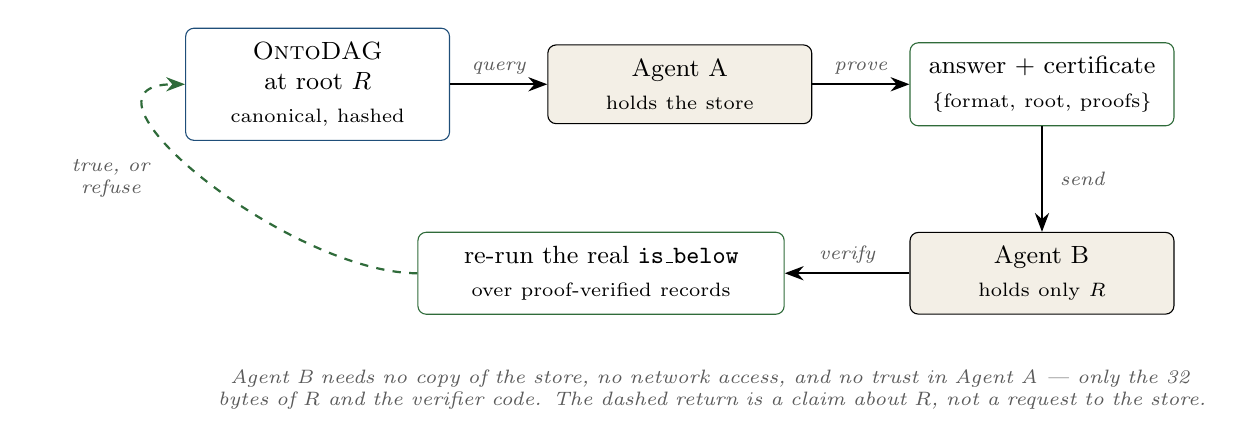
\begin{tikzpicture}[font=\small,
  b/.style={draw, rounded corners=3pt, align=center, inner sep=5pt,
            minimum height=1.0cm, text width=3.0cm},
  ar/.style={-{Stealth[length=2.4mm]}, thick},
  lab/.style={font=\scriptsize\itshape, text=odgrey, align=center}]

\node[b, draw=odblue] (store) at (0,0)
  {\odag{} at root $R$\\[1pt]\scriptsize canonical, hashed};
\node[b, fill=odsand] (a1) at (4.6,0)
  {Agent A\\[1pt]\scriptsize holds the store};
\node[b, draw=odgreen] (cert) at (9.2,0)
  {answer $+$ certificate\\[1pt]\scriptsize
   \{format, root, proofs\}};
\node[b, fill=odsand] (a2) at (9.2,-2.4)
  {Agent B\\[1pt]\scriptsize holds only $R$};
\node[b, draw=odgreen, text width=4.3cm] (check) at (3.6,-2.4)
  {re-run the real \cmd{is\_below}\\[1pt]\scriptsize
   over proof-verified records};

\draw[ar] (store) -- node[lab, above]{query} (a1);
\draw[ar] (a1)    -- node[lab, above]{prove} (cert);
\draw[ar] (cert)  -- node[lab, right, xshift=1mm]{send} (a2);
\draw[ar] (a2)    -- node[lab, above]{verify} (check);
\draw[ar, odgreen, dashed] (check.west) to[out=180, in=180, looseness=1.1]
  node[lab, left, xshift=-1mm, text width=1.9cm]{true, or\\refuse} (store.west);

\node[lab, text width=12.5cm, anchor=north] at (5.0,-3.5)
  {Agent B needs no copy of the store, no network access, and no trust in
   Agent A --- only the 32 bytes of $R$ and the verifier code. The dashed
   return is a claim about $R$, not a request to the store.};
\end{tikzpicture}
\caption{Verification without disclosure. Because the root commits to the
whole state and the encoding is canonical, a subsumption answer can be
shipped with everything needed to check it.}
\label{fig:verify}
\end{figure}

\subsection{Writing: propose, echo, confirm}

Letting agents \emph{write} raises different problems. \odag{}'s write surface
answers three of them structurally.

\paragraph{Idempotence, by construction.} Re-filing the same fact is a graph
no-op: the same root comes out. An agent that retries after a timeout, or two
agents that independently reach the same conclusion, cannot corrupt anything.
This falls straight out of the canonical form --- it is not a feature that had
to be built.

\paragraph{Compare-and-confirm.} A write is two steps. \cmd{propose\_put}
returns the canonical echo (what the stored spellings will be, which claims
this implies, what is already true, which parents do not exist) plus a
\emph{proposal token}: a hash of the operation, the canonicalised terms, and
the current root. \cmd{put} recomputes the token; if the store has moved or a
spelling resolved differently, it refuses and asks the agent to propose again.

This matters more for agents than for humans. An agent may spend many seconds
of reasoning between reading and writing, during which the store can move; and
it cannot notice a surprise the way a person glancing at a terminal would.
Making the surprise into a refusal is the difference between a race and an
error message.

\paragraph{Every write is a speech act.} A successful write commits two
things: the knowledge change, and one signed provenance record per claim,
recording the author's key, the claim (a canonical
$\mathit{sub} \dsub \mathit{sup}$ pair), and the root the author was looking
at when they decided. Removals emit retraction records: retracting is also
something somebody did.

Notice where the signature goes. It is in a \emph{separate} store with its own
root, never inside the knowledge records --- because if authorship were part
of the hashed knowledge, two people who know the same thing would get
different roots, and G1 would be gone. \emph{Who said it} and \emph{what is
said} are deliberately different objects with different addresses.

\subsection{The review problem}
\label{sec:agents-review}

Here is the problem that will dominate agent-written knowledge, and it is not
a technical one:

\begin{keyidea}
Agents write faster than anyone can review. A store that accepts machine
writes at machine speed accumulates claims nobody has checked, and the value
of the store degrades to the value of its least careful writer.
\end{keyidea}

\odag{} offers three partial answers and one promising direction.

\paragraph{Attribution makes the problem tractable rather than solving it.}
Because every claim is signed, a reader can filter: accept claims from these
keys, ignore the rest. Standing is computed from verified records only, and
retraction is sticky per author. Forged records are listed but never counted.
This does not check anything; it makes \emph{whose} unchecked claims you are
carrying an explicit decision.

\paragraph{Endorsement is a separate speech act.} A reviewer can endorse a
claim without touching the knowledge graph. Reviewing is thus recorded work
that accumulates, rather than an event that happens once in a chat window and
is lost.

\paragraph{Disagreement is queryable structure.} If disjointness claims are
ever adopted, an inconsistency arriving by merge is not an error condition; it
is a non-empty \cmd{get(Cat, Dog)}. The consistency check is the query
primitive again --- which means finding the mess an agent made is the same
operation as using the store.

\paragraph{The direction: bound and order the review.}
Section~\ref{sec:learn-exploration} argued that attribute exploration is the
right shape here, and the reason belongs in this section. Exploration inverts
the flow: instead of the agent proposing arbitrary edits which a human must
review in arbitrary order, the \emph{system} computes the next question that
is not already answered, and the agent answers it. The review queue becomes
minimal (no redundant questions), ordered (each maximally informative given
the answers so far), and terminating. That is the difference between review
that scales and review that does not.

\subsection{Agents sharing memory}

The multi-agent case is where the properties compound, and it is worth a
concrete scenario.

Two agents work on the same domain on different machines, offline from each
other. Each files what it learns. Later they exchange roots.

\begin{enumerate}[leftmargin=1.7em]
\item If the roots are equal, they know the same things. \emph{One comparison,
  32 bytes, no data transferred} --- and because canonicality is semantic, this
  works even if they built their stores in different orders, by different
  routes, spelling values differently.
\item If the roots differ, a structural diff localises the disagreement to the
  exact differing records, without downloading either store wholesale.
\item Merging converges: each folds in the other's root and both reach the
  byte-identical result, whatever order the exchange happened in (G5). No
  server, no consensus, no lock.
\item Afterwards, each can ask ``which of these claims came from the other
  agent, and do I trust that key?'' --- because the provenance store merged
  too, conflict-free, by the same union rule.
\end{enumerate}

Compare the same scenario with two agents holding vector stores, or two
fine-tuned models: there is no equality test, no diff, no merge, and no
attribution. There is only ``ask them both and hope''.

\subsection{Token economics, briefly}

A practical point that matters at scale. An exact query returns exactly the
relevant items and a count. An approximate retrieval returns $k$ chunks chosen
by similarity, of which some are relevant, and the agent pays context tokens
for all of them and then reasons about which to believe. For queries that are
genuinely conjunctive --- ``refundable, in Japan, booked before March'' ---
the exact path is both cheaper and correct, and the cost difference grows with
the store.

The same applies to structure. An agent that needs to know what a store
contains can read a \cmd{about} record of a few hundred tokens rather than
sampling documents. Discoverability is a token-efficiency feature as much as a
correctness one.

\subsection{What \odag{} does not solve}

An honest list, because the value of the guarantees depends on not
overstating them.

\begin{itemize}[leftmargin=1.4em]
\item \textbf{Proofs attest structure, never truth.} Every certificate proves
  what was asserted and what follows from it --- never that the assertion is
  true of the world. That is the oracle problem, and no data structure solves
  it. The available answers are social (attribution and endorsement) and
  economic (Section~\ref{sec:crypto-bonds}).
\item \textbf{Classification is not automatic.} \odag{} has no defined
  concepts (\S\ref{sec:meet-trap}), so nothing places an item in the right
  category for you. That job falls to the agent --- which is a reasonable
  division of labour in 2026, but it means the quality of the store depends on
  the quality of the classifier.
\item \textbf{Names must be agreed.} Two agents using different words for the
  same idea produce two nodes, and no mechanism notices. This is the price of
  Section~\ref{sec:keep-names}, and it is real.
\item \textbf{No relations.} ``Alice authored Doc1'' cannot be said. Agents
  will try; the surface logs what they fail to express, which is how the
  system will learn whether the wall needs moving.
\item \textbf{Retraction does not travel.} A peer who still holds a removed
  edge re-adds it on merge. Single-writer and publish-to-readers deployments
  keep removals; concurrent writers do not.
\end{itemize}

\section{Why this matters for cryptographic and decentralised systems}
\label{sec:crypto}

The second constituency wants the same four properties as the first, for
different reasons. An agent wants canonical, addressable, verifiable,
attributable knowledge because it cannot trust its own memory. A decentralised
system wants it because there is no server to trust.

\subsection{The gap content addressing leaves}

Content-addressed storage --- Merkle structures \citep{merkle1987}, IPFS
\citep{benet2014}, Ethereum Swarm \citep{tron2020} --- solved integrity and
made durable, host-independent references possible. A hash names exactly one
immutable byte string, forever, and tampering is detectable on retrieval.

What it did not solve is \emph{meaning}. A 32-byte reference tells you nothing
about what the content is or how it relates to anything else. The standard
answer has been the manifest: a mapping from path names to references --- in
other words, a directory tree. And a directory tree is the wrong shape for the
same reason it was always the wrong shape: every object must live in exactly
one place, while almost everything worth storing is legitimately several
things at once. \texttt{outbound.pdf} is a flight document, a Japan document,
and a refundable booking; a tree makes you choose, or makes you duplicate.

\begin{figure}[h]
\centering
\begin{subfigure}[b]{0.47\textwidth}\centering
  \dotfig[0.82]{folder_tree}
  \caption{A tree must choose. The Paris flight is under
  \textsf{Flights}; the Japan one is under \textsf{Japan} --- so
  ``all flights'' needs a duplicate.}
\end{subfigure}\hfill
\begin{subfigure}[b]{0.47\textwidth}\centering
  \dotfig[0.82]{dag_multiparent}
  \caption{A DAG does not. \texttt{outbound.pdf} is under both, once, and
  the query decides which view you get.}
\end{subfigure}
\caption{The manifest problem in one picture.}
\label{fig:tree-vs-dag}
\end{figure}

\odag{} is a semantic layer for exactly this gap: a small structure that
records \emph{what things are}, independently of where their bytes live, and
that happens to have the one property content-addressed storage rewards above
all others.

\subsection{Semantic content addressing}

\begin{keyidea}
Ordinary content addressing gives \textbf{same bytes, same hash}. \odag{}
gives \textbf{same meaning, same hash}.
\end{keyidea}

That upgrade is the whole contribution, and it is worth spelling out what it
takes. Two people file the same six documents. They do it in different orders.
One of them types a few redundant links along the way. One writes
$400\,\mathrm{g}$ and the other $0.4\,\mathrm{kg}$. Ordinary content
addressing gives them two different hashes, because their bytes differ.
\odag{} gives them one, because:

\begin{itemize}[leftmargin=1.4em]
\item the transitive reduction is unique, so build order and redundant edges
  are quotiented away (Thm~\ref{thm:unique-reduction});
\item values are canonicalised by denotation, so spelling is quotiented away;
\item the serialisation and the storage trie are canonically encoded, so
  nothing about \emph{how} the store was written survives into the bytes.
\end{itemize}

The consequences are unusual enough to list, because no mainstream database
offers them:

\begin{enumerate}[leftmargin=1.7em]
\item \textbf{Deduplication of meaning.} Two organisations that independently
  build the same taxonomy converge on one address, and discover it by
  comparing 32 bytes.
\item \textbf{Agreement is a hash comparison.} ``Do we share an ontology?''
  costs one string comparison and zero data transfer. Because canonicality is
  semantic, this is same-\emph{meaning}-same-hash, not
  same-\emph{bytes}-same-hash.
\item \textbf{A root is a commitment.} Publishing a root commits you to an
  entire knowledge state, in the cryptographic sense: you cannot later change
  what you knew without changing the reference. This is a commitment scheme
  you get for free, without designing one.
\item \textbf{Snapshots are free and eternal.} Nothing is overwritten, so
  every past root still resolves. ``What did the catalogue say on the day of
  the contract?'' is answerable years later.
\item \textbf{Disagreement localises.} Two differing roots can be narrowed to
  the exact differing records by structural diff, without transferring either
  store.
\end{enumerate}

\subsection{Convergence without consensus}

This is the property that makes \odag{} suit decentralised infrastructure
rather than merely tolerate it, and it deserves emphasis because it is
frequently assumed to be impossible.

Distributed systems usually achieve agreement by \emph{consensus}: a protocol
(or a blockchain) that decides an order of operations. Consensus is expensive,
requires liveness, and requires participants to be online together.

\odag{} needs none of it. Merge is commutative and idempotent
(Thm~\ref{thm:merge}), so replicas that have seen the same set of updates ---
in any order, with any duplicates --- hold identical state. This is the
defining property of a state-based CRDT \citep{shapiro2011}, and combined with
content addressing it gives the pattern \citet{sanjuan2020} call a
Merkle-CRDT: state identified by hash, merged by a convergent function,
gossiped rather than ordered, and which is the substrate the local-first
software argument \citep{kleppmann2019} asks for: full local capability,
collaboration without a coordinating server, and no vendor holding the
authoritative copy.

\begin{keyidea}
Two writers who fold in each other's published roots reach the
\emph{byte-identical} root regardless of gossip order (G5). No server, no
chain, no lock, no coordination --- and afterwards they can \emph{prove} they
agree by comparing the root.

The blockchain, when one is involved at all, is therefore not needed for
agreement. It is needed only for the things chains are actually good at:
timestamping, settlement, and adjudicating disputes about money.
\end{keyidea}

The price is stated in Section~\ref{sec:merge} and repeated here because it is
the one thing an integrator must design around: merge is union, so it is
grow-only. A removal can be resurrected by a peer holding the old state.
Undoing is local. Any application that needs authoritative deletion must add
its own layer.

\subsection{Publishing, following, and paying rent}
\label{sec:crypto-economics}

Concretely, on Swarm \citep{tron2020}, an \odag{} store becomes:

\begin{center}\small
\begin{tabularx}{\textwidth}{@{}p{4.2cm} X@{}}
\toprule
\textbf{Swarm mechanism} & \textbf{What \odag{} uses it for}\\
\midrule
chunks, retrieved by hash & the record blobs and trie nodes: one commit
  writes only what changed\\
postage stamps (storage rent) & keeping a published ontology alive; and, more
  interestingly, \emph{not} keeping derived indexes alive\\
signed feeds & a followable address for ``the latest root published by this
  key'' --- mutability on top of immutability\\
retrievability checks & confirming a published ontology is actually fetchable
  by strangers\\
\bottomrule
\end{tabularx}
\end{center}

The postage mechanism produces a genuinely elegant fit with the derived-layer
discipline of Section~\ref{sec:keep}. Derived structures --- cone summaries,
implication lints, MDL-learned concepts, materialised meets --- are
regenerable by definition. On a network where storage costs rent, that gives
eviction a native mechanism:

\begin{keyidea}
\textbf{Let a derived index's postage lapse.} A cache whose eviction policy is
``stop paying'' is a cache with an honest cost model: an index is kept warm
exactly as long as query traffic justifies its rent, and its disappearance
costs nothing but recomputation. Regenerable things are allowed to die.
\end{keyidea}

This also gives the workload-optimal materialisation problem of
Section~\ref{sec:dir-materialisation} a real objective function rather than a
notional one: the space term is not a tuning constant, it is money.

\subsection{Anchoring, and settling disputes}

A root is 32 bytes, which is exactly the size of one storage word in the
Ethereum Virtual Machine. Putting a root in a contract or an event log is a
timestamped commitment to a whole knowledge state, at negligible cost.

What that enables is dispute resolution by proof rather than by argument:

\begin{enumerate}[leftmargin=1.7em]
\item A party publishes a catalogue and anchors its root on chain.
\item A counterparty acts on a claim about the catalogue --- ``this item is
  under $5\,\mathrm{kg}$ and located in the EU''.
\item If the claim is disputed, it is settled by exhibiting a proof against
  the anchored root. Inclusion, absence and subsumption all have proofs
  (\S\ref{sec:agents-verify}).
\end{enumerate}

Two practical tailwinds are worth recording. Swarm's addressing is
keccak-based --- the EVM's native hash --- so on-chain verification of a
Swarm-side inclusion proof does not require an expensive foreign hash
function; and Swarm's own storage-incentive machinery already verifies such
proofs on chain, so the pieces exist.

One honest gap, though. \odag{}'s current subsumption certificates work by
\emph{re-execution over authenticated records}, which is ideal off-chain
(semantics stay single-sourced in the real implementation) and impractical
on-chain (a contract cannot re-run a graph traversal). The shape that a
contract \emph{can} check is a hash-link path: a Merkle-ised index over the
semantic graph, where a positive subsumption is a self-verifying chain of
hashes. That is a known, designed-but-unbuilt extension, and it is the right
thing to build when --- and only when --- somebody actually needs a
subsumption verified on chain.

\subsection{Bonded claims: the economic third leg}
\label{sec:crypto-bonds}

Limit L1 says proofs attest structure, never truth. Attribution
(Section~\ref{sec:agents}) upgrades that to ``someone said it, and you may
choose whose word you take''. There is a third leg available, and it is
economic: \emph{someone will pay if it is wrong}.

A sister project (\texttt{factbond}, design stage) explores bonded assertions:
a stake slashed on successful dispute, a premium that prices reliability.
Whatever the details, two structural gifts flow from \odag{}'s side of the
fence and are worth naming because they are unusual:

\begin{itemize}[leftmargin=1.4em]
\item \textbf{Claim identity is free and canonical.} Bonding a claim requires
  naming it unambiguously. A root plus a canonical claim is exactly that ---
  and because a root commits to the whole store, a single bond can cover
  millions of facts, with any individual one disputed later by an inclusion
  proof. \emph{Batched commitment, itemised dispute.}
\item \textbf{One class of dispute adjudicates mechanically.} Distinguish
  ``matches-source'' claims (``the store at root $R$ entails $X$'') from
  ``matches-world'' claims (``$X$ is true''). The first is settled by a Tier-2
  certificate --- a proof checker is the cheapest possible rung of a dispute
  ladder, and it needs no human and no oracle. Only matches-world claims need
  evidence and adjudicators.
\end{itemize}

That split is only available because subsumption is decidable from the stored
graph plus exact arithmetic. It is a direct dividend of the refusals in
Section~\ref{sec:keep}.

\subsection{Marketplaces: matching as cone intersection}

A second sister project (\texttt{loopmarket}) uses \odag{} for marketplace
matching, and it is the application that forced typed values into existence.
A courier's constraint --- ``anything up to $5\,\mathrm{kg}$, collected in
this region, delivered before Friday'' --- must match offers nobody
pre-classified against that threshold.

Three properties of the result matter for a crypto audience:

\begin{itemize}[leftmargin=1.4em]
\item \textbf{Matching is the query primitive.} A constraint is a query term,
  so matching is one cone intersection --- one planner, one merge story, no
  second filtering mechanism beside subsumption.
\item \textbf{Recall-completeness is guaranteed, not hoped for.}
  \cmd{get\_overlapping} returns every value whose denotation provably
  intersects the constraint's (G6). For a marketplace, ``we did not miss a
  match'' is a property worth being able to state.
\item \textbf{No floats, anywhere.} Values are exact rationals of an SI anchor
  unit. This is the same discipline crypto already uses for money --- wei,
  satoshi, integer base units --- adopted for the same reason: exactness by
  construction rather than by careful rounding.
\end{itemize}

\subsection{The zero-knowledge direction}
\label{sec:crypto-zk}

The natural next question for a privacy-sensitive counterparty is: can I prove
``my catalogue contains something under $\mathrm{weight}(..5\mathrm{kg})$ and
$\mathrm{location}(\mathrm{EU})$'' \emph{without revealing the catalogue}?

This is the zero-knowledge question in its original sense
\citep{goldwasser1989}: convince a verifier that a statement holds while
revealing nothing beyond its truth. It is heavy research --- succinct proofs
over trie walks --- and \odag{} deliberately walls it until a real consumer appears. But the positioning is
worth recording, because \odag{} is unusually well suited when the time comes:

\begin{itemize}[leftmargin=1.4em]
\item deterministic canonical encoding: the statement being proved is about a
  well-defined object, not about one serialisation among many;
\item one query primitive: a single circuit shape covers the whole query
  language;
\item \textbf{no floating point anywhere} --- values are pairs of integers.
  Arithmetic circuits are built over finite fields, where rationals are
  natural and floats are a nightmare. \odag{}'s exactness commitment
  (\S\ref{sec:keep}), adopted for canonicality, turns out to be exactly the
  property a proof system wants.
\end{itemize}

That last point is a good illustration of a theme in this paper: the refusals
compound. Refusing floats to protect canonical roots also made the structure
circuit-friendly, years before anyone asked.

\subsection{Governance: canonical forms, plural}

A final point, less technical but arguably the most important for a
decentralised deployment.

Every attempt at a single official classification of the world has failed, and
Borges gave the argument its definitive form: since we do not know what the
universe is, every classification of it is arbitrary and conjectural
\citep{borges1942}. Foucault made the historical version of the same point ---
classification schemes are not refined over time so much as replaced.

The constructive reading, for a system design, is that \emph{no single
taxonomy deserves to be baked into identity}. \odag{}'s answer is
architectural rather than editorial:

\begin{itemize}[leftmargin=1.4em]
\item there is no official store --- anyone publishes a root;
\item vocabularies travel \emph{inside} stores as ordinary declarations, so
  adopting a vocabulary is merging a published root, not installing software;
\item adoption is by explicit reference to a root, so what you adopted is
  exactly what you can name and check;
\item disagreement is representable: two communities may hold divergent
  overlays of a shared core and both be well-formed.
\end{itemize}

Wilkins wanted the one true tree. The answer here is closer to Borges:
canonical \emph{forms}, plural --- one per community, per purpose, per moment
--- each canonical in itself, each mergeable with the others, and none final.

\subsection{Honest limits, again}

\begin{itemize}[leftmargin=1.4em]
\item \textbf{L1: proofs attest structure, never truth.} No amount of
  cryptography makes an assertion true. Attribution and bonds change the
  incentives, not the epistemology.
\item \textbf{L2: everything is relative to a pinned interpretation context.}
  A proof about a typed value must pin the declarations and the registry
  version. A verifier running different arithmetic must refuse rather than
  misinterpret --- and \odag{}'s certificates do refuse.
\item \textbf{Grow-only merge} remains the standing constraint on any
  multi-writer deployment.
\item \textbf{The infrastructure wall is real.} Running a node, funding it,
  and buying storage rent is a genuine barrier --- measured in this project's
  own logs at minutes-to-hours for a first-time user, not seconds. The
  practical response has been to make the interesting properties available
  \emph{before} the network step: a local content-addressed store gives
  canonical roots, snapshots, certificates and merge with no node at all, so
  the ideas can be evaluated before the infrastructure is confronted.
\end{itemize}


% ===========================================================================
\part*{Part V --- Directions}
\addcontentsline{toc}{part}{Part V --- Directions}
% ===========================================================================

\section{Directions}
\label{sec:directions}

This section maps what the comparison opens up. Items are grouped by how much
has to be invented before they can be built, and each carries the same four
labels used in Section~\ref{sec:learn}: what it is, what it buys, what it
costs, and which invariant it puts at risk.

A caution first, which is this project's own standing discipline and is worth
inheriting: \emph{nothing here is scheduled by virtue of being written down}.
Each item is recorded with the trigger that would signal it has become
necessary, so that a future reader recognises the moment instead of
pre-building for it.

\subsection{The organising picture}

Almost everything below is a point on one line, so it is worth drawing the
line first.

\begin{figure}[h]
\centering
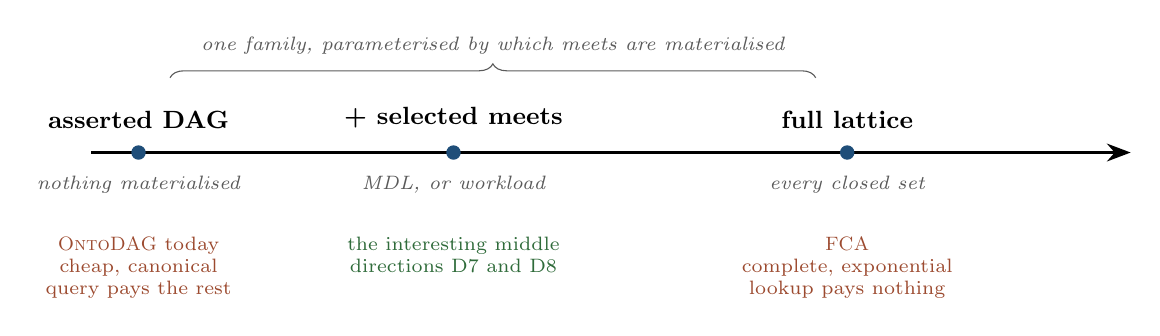
\begin{tikzpicture}[font=\small]
% the spectrum bar
\draw[very thick, -{Stealth[length=3mm]}] (0,0) -- (13.2,0);
\foreach \x/\lab/\sub in {
   0.6/{asserted DAG}/{nothing materialised},
   4.6/{+ selected meets}/{MDL, or workload},
   9.6/{full lattice}/{every closed set}}
  {\filldraw[odblue] (\x,0) circle (2.4pt);
   \node[anchor=south, align=center, font=\small\bfseries]
     at (\x,0.18) {\lab};
   \node[anchor=north, align=center, font=\scriptsize\itshape, text=odgrey]
     at (\x,-0.18) {\sub};}
\node[anchor=north, align=center, font=\scriptsize, text=odrust]
  at (0.6,-0.95) {\odag{} today\\cheap, canonical\\query pays the rest};
\node[anchor=north, align=center, font=\scriptsize, text=odgreen]
  at (4.6,-0.95) {the interesting middle\\directions D7 and D8};
\node[anchor=north, align=center, font=\scriptsize, text=odrust]
  at (9.6,-0.95) {\fca{}\\complete, exponential\\lookup pays nothing};
\draw[decorate, decoration={brace, amplitude=5pt}, odgrey]
  (1.0,0.95) -- (9.2,0.95)
  node[midway, above=5pt, font=\scriptsize\itshape, text=odgrey]
  {one family, parameterised by which meets are materialised};
\end{tikzpicture}
\caption{\odag{} and \fca{} are the two endpoints of a single family, not two
rival data structures. A member of the family is: the asserted graph, plus a
set of materialised meets, plus a storage mode per cone. \odag{} materialises
none and pays at query time; \fca{} materialises all and pays in space. The
research question is which middle point a given workload wants.}
\label{fig:spectrum}
\end{figure}

Seeing it this way reframes several apparently separate questions as one.
``Which concepts should MDL learn?'', ``which cones should be indexed?'',
``which meets should the query planner materialise?'' and ``which categories
should a user be prompted to create?'' are the same question asked by four
different subsystems.

\subsection{Buildable now}

These need no new theory and threaten no invariant.

\paragraph{D1. Re-describe dimensions as an interval pattern structure.}
\emph{Cost: an afternoon of writing.} Section~\ref{sec:learn-patterns} showed
\odag{}'s typed values are an instance of \citet{ganter2001}. Recording that
in the design documents converts an engineering hunch into a known-correct
construction, gives the multi-coordinate question a ready answer (product
semilattice, componentwise meet), and supplies the projection theory that the
future per-dimension index will need. Highest value-to-cost ratio in the
paper.

\paragraph{D2. An ordinal kind.} \emph{Trigger: someone files ranks.} The
scale table of Section~\ref{sec:learn-scaling} has a hole where
\textsf{beginner} $<$ \textsf{intermediate} $<$ \textsf{expert} should be.
Declaring an ordinal chain is monotone and canonicalisable, so it passes both
admissibility axes. Build it with the arithmetic deliberately \emph{absent},
because the standing hazard with ordinal data is people averaging ranks
\citep{stevens1946}.

\paragraph{D3. Reduced labelling in the visualiser.} \emph{Cost: a rendering
change.} Compare Figures~\ref{fig:lattice} and~\ref{fig:ontodag}: the same
information, far less ink. Worth most on stores with many typed values.

\paragraph{D4. An implication lint.} \emph{Trigger: users mis-filing things
that the store's own contents would have caught.} Compute extensional
implications over a pinned root into a derived store; surface them as prompts.
Never store them as claims (\S\ref{sec:learn-implications}). The natural first
version is single-premise implications only, which are cheap --- one closure
per category.

\paragraph{D5. Cone bitmaps behind \cmd{get}.} \emph{Trigger: queries
measurably hot.} An in-memory bitmap per category, intersected with a bitwise
\textsc{and}. Bounded, dependency-free (Python integers suffice), invisible in
the schema, and it has a free test oracle: the population count of a cone
bitmap must equal the maintained \verb|descendant_count|. This is the first
step of the semantic-codes programme and the one that needs no decisions. When
it outgrows plain integers the prior art is well mapped: compressed bitmaps
\citep{lemire2018} for the representation, and interval labelling
\citep{agrawal1989} for the trick of numbering nodes so that a cone becomes a
few contiguous ranges.

\subsection{Medium term: needs a design, not a discovery}

\paragraph{D6. Attribute exploration with a language model as the expert.}
\label{sec:dir-exploration}
\emph{Trigger: available now; the blocker is willingness, not knowledge.}

This is the most promising item in the paper, and
Sections~\ref{sec:learn-exploration} and~\ref{sec:agents-review} argued why:
it is the only proposal here that makes review of machine-written knowledge
\emph{bounded, ordered and terminating}. A concrete v1 for the single-writer
case:

\begin{enumerate}[leftmargin=1.7em,itemsep=1pt]
\item Pin a root. Everything that follows is relative to it, so the session is
  reproducible and citable.
\item View the store as the context $\ctx(P)$ of Section~\ref{sec:dictionary}
  and compute the next unconfirmed implication by NextClosure
  \citep{ganter1984}.
\item Ask the agent, over the MCP surface, in domain language: \emph{is every
  X also a Y?}
\item \textbf{Yes} $\to$ record a signed confirmation in the provenance store.
  If the implication has a single-category premise it is also a subsumption,
  so offer it as an ordinary \cmd{put}.
\item \textbf{No} $\to$ require a counterexample, and file it with \cmd{put}.
  The store grows by exactly the object that refutes the question.
\item Terminate when no unconfirmed implications remain. Present the human
  with the confirmed base --- which is minimal and non-redundant by
  construction.
\end{enumerate}

Two properties make this more than a demo. The counterexample requirement
means a \emph{No} is as informative as a \emph{Yes} --- the store improves
either way, which is not true of ordinary agent review. And because every
answer is a signed claim against a pinned root, a later reader can see
precisely which questions this author answered, and re-run the exploration
under a different author to compare.

Open sub-problem: a wrong expert. Classical exploration assumes infallibility;
attribution degrades the guarantee honestly to ``complete relative to what
this author asserted'', which is the right weakening. A second agent
re-answering the same question sequence, with disagreements surfaced, is the
obvious cheap defence and would be worth measuring.

\paragraph{D7. Workload-optimal materialisation.}
\label{sec:dir-materialisation}
\emph{Trigger: a real query log.} Figure~\ref{fig:spectrum}'s middle, stated
as an optimisation problem: choose a set $M$ of materialised meets and a
storage mode per cone to minimise
\[
  \mathbb{E}_{q \sim Q}\bigl[\text{retrieval cost}(q; M)\bigr]
  \;+\; \lambda_{\text{space}}\cdot \text{storage}(M)
  \;+\; \lambda_{\text{maint}}\cdot \text{update cost}(M).
\]
This is a known problem three times over: view-materialisation selection on a
lattice \citep{harinarayan1996}, whose greedy solution is near-optimal by
submodularity; retrieval-aware MDL, which is the same objective seen from the
learner's side; and adaptive indexing \citep{idreos2007}, which supplies the
online algorithm --- every query that computes a residual intersection has
just computed a candidate meet, so admit it when expected reuse covers its
cost and evict when cold.

Two \odag{}-specific notes. The selectivity statistics the greedy algorithm
needs already exist and are exact (\verb|descendant_count|). And the space
term is not a tuning constant on a rent-charging network: it is postage
(\S\ref{sec:crypto-economics}).

\emph{The soundness condition, which is easy to miss:} materialised meets may
be used to \emph{prune} candidates but not to \emph{generate} them, unless
placement is made canonical --- because of the meet-substitution trap
(\S\ref{sec:meet-trap}). A node under $A$ and $B$ is not the meet of $A$ and
$B$.

\paragraph{D8. MDL-learned concepts, with a promotion path.}
\label{sec:dir-mdl}
\emph{Trigger: a store big enough that nobody can see its structure.} Run the
learner \citep{mdlfca} over a pinned root; keep its output in a derived store;
let a human or an accountable agent promote a learned category into the shared
graph as an ordinary claim recording the root it was derived from. The
layering is what keeps this safe (\S\ref{sec:learn-mdl}), and the promotion
step is what keeps it attributable.

The interesting scientific question underneath is whether MDL-selected
concepts agree with the ones people actually name. That is a measurable
question --- take a hand-built ontology, hide the intermediate categories,
learn from the leaf assignments, compare --- and nobody appears to have run
it at scale.

\paragraph{D9. Merkle-ised cone commitments.} \emph{Trigger: somebody needs a
subsumption verified on chain.} A per-node cone-commitment index, in its own
store, manifest-pinned, deterministic from the canonical form. It buys
path-sized order-free positive proofs, per-category agreement by one hash
comparison, and the one proof shape a contract can check
(\S\ref{sec:crypto}). It can never be the base representation --- names are
identity, and a Merkle address changes whenever anything below the node
changes --- so it is an index over the named graph, forever.

\paragraph{D10. The thin browser client.} \emph{Trigger: a published store
anyone should be able to query without downloading.} Most pieces exist: a
lazy reader that fetches records as a query walks them, published cone
summaries that collapse broad queries to a handful of fetches, and a base
install that is pure Python. The remaining work is batching the fetch frontier
and bridging to network access from inside a browser sandbox.

\subsection{Longer term: genuinely open}

\paragraph{D11. Concurrent exploration.} Two agents exploring two replicas ask
different questions and confirm different things. Since exploration assumes a
fixed universe and \odag{} assumes a merging one, reconciling them is open.
A promising angle: exploration confirmations are claims, claims merge
conflict-free, and the \emph{question} sequence is a derived, local artefact
--- so perhaps only the answers need to converge, and each replica may
legitimately have asked a different route to them.

\paragraph{D12. Relations.} The biggest wall. ``Alice authored Doc1'' is not
subsumption, and no amount of cleverness makes it one. Two things are known.
The \fca{}-native answer, Relational Concept Analysis
\citep{rouanehacene2013}, computes a global fixpoint, which conflicts with
local canonical form. And the description-logic answer \citep{baader2003}, an EL-shaped
extension, is \emph{monotone} --- so merge would survive --- but makes
subsumption a global inference, so canonicalising up to logical equivalence
means canonicalising an entailment closure. That is the axis that breaks, and
naming it precisely is the contribution of Section~\ref{sec:two-canonical-forms}:
the guarantee would silently degrade from ``equal knowledge, equal root'' to
``equal syntax, equal root'', which is the weaker thing consumers would
mistakenly keep relying on. Anyone attempting this should treat cheap semantic
canonicalisation of the fragment as the \emph{primary} research problem, not
tractability of reasoning.

There is a precise precedent for drawing a line this way: EL++ retains
polynomial subsumption only under ``p-admissible'' concrete domains
\citep{baader2005} --- the description-logic community's version of \odag{}'s
rule that only exact-arithmetic kinds may enter the canonical order.

\paragraph{D13. Zero-knowledge subsumption.} \emph{Trigger: a
privacy-demanding counterparty.} Positioned in Section~\ref{sec:crypto-zk};
the encouraging part is that the properties a circuit wants --- determinism,
one primitive, no floats --- were already bought for other reasons.

\paragraph{D14. Products of DAGs, and factorial codes.} This one returns to
the origin. Section~\ref{sec:neural} described a code whose active units carry
a category structure; the natural next question from the coding side is
whether that structure \emph{factors} --- whether the code decomposes into
independent groups of units, each carrying its own small DAG, so that an
item's description is a tuple rather than a set. That is a factorial code in
Barlow's sense \citep{barlow1989}, a product lattice in order-theoretic terms,
and a product of pattern structures in \fca{} terms.

\odag{} already has a degenerate version: its dimensions are exactly such
independent factors (weight, time and location vary independently, and a value
in one says nothing about the others). Generalising from a handful of declared
dimensions to \emph{learned} factors would connect the MDL programme to the
redundancy-reduction tradition it came from, and would give the surface layer
a principled account of when two categories are ``about the same thing''.
The machine-learning neighbours to read first are the layer-wise
total-correlation approach of \citet{versteeg2014} and the unbounded-depth
Bayesian prior over binary latent DAGs of \citet{adams2010}.

\paragraph{D15. Continuous relaxations as a recall layer.} Order embeddings
\citep{vendrov2016} and hyperbolic embeddings \citep{nickel2017} learn vectors
in which subsumption is coordinate dominance or radial position. They are the
approximate, differentiable cousins of the ancestor-set code, and they fail in
exactly the way the exact structure does not: approximately. That makes them a
natural \emph{proposal} layer over an exact \emph{disposal} layer, which is
precisely the division of labour Section~\ref{sec:agents} recommends for
retrieval. Worth noting that the tree/DAG obstruction reappears there too ---
trees embed in hyperbolic space with arbitrarily low distortion, DAGs only
approximately.

\paragraph{D16. Closing the mind--brain loop.} The most speculative and, for
this project's origins, the most fitting. Figure~\ref{fig:mind-brain} has two
directions and the literature has mostly travelled one of them: from recorded
codes to concept lattices \citep{endres2008,endres2010}. The other direction
is now buildable: take an ontology, embed it as an ancestor-set code
(Proposition~\ref{prop:roundtrip} says nothing is lost), and ask whether a
population code with that structure predicts responses better than one
without. \odag{} would be supplying the ontology in a form where the embedding
is exact and reproducible --- which is to say, canonical --- and where two
laboratories could confirm they used the identical ontology by comparing 32
bytes.

\subsection{The map}

\begin{table}[h]\centering\small
\caption{All directions, with the trigger that would justify starting.}
\label{tab:directions}
\vspace{1mm}
\begin{tabularx}{\textwidth}{@{}p{0.7cm} p{4.5cm} p{2.2cm} X@{}}
\toprule
& \textbf{Direction} & \textbf{Risk to invariants} & \textbf{Trigger}\\
\midrule
D1 & Pattern-structure framing & none & now (free)\\
D2 & Ordinal kind & none & someone files ranks\\
D3 & Reduced labelling & none & now\\
D4 & Implication lint & none (derived) & users mis-filing\\
D5 & Cone bitmaps & none (derived) & queries hot\\
\midrule
D6 & Exploration with an LLM expert & none (claims) & now; the best fit with
     agents\\
D7 & Workload materialisation & soundness caveat & a real query log\\
D8 & MDL concepts + promotion & none (derived) & store too big to see\\
D9 & Merkle cone commitments & none (derived) & on-chain subsumption needed\\
D10 & Thin browser client & none & a published store worth reading\\
\midrule
D11 & Concurrent exploration & unclear & multi-writer exploration\\
D12 & Relations & \textbf{breaks canonicality} & mass reification observed\\
D13 & Zero-knowledge subsumption & none & a private counterparty\\
D14 & Products of DAGs & none (derived) & research\\
D15 & Embeddings as recall & none (outside) & vague-input queries\\
D16 & Ontology $\to$ neural code & none & a collaborator with data\\
\bottomrule
\end{tabularx}
\end{table}

Only one row in that table says ``breaks canonicality'', and it is the one
everybody asks for first. That is the paper's practical warning, and
Section~\ref{sec:conclusion} makes it the closing point.

\section{Conclusion}
\label{sec:conclusion}

The question this paper set out to answer was how \odag{} relates to Formal
Concept Analysis. The answer turned out to be more specific than expected, and
more useful.

\paragraph{They compute the same function.} \fca{}'s derivation operator on
attribute sets \emph{is} \odag{}'s query primitive:
$B' = \cmd{get}(B)$, exactly (Proposition~\ref{prop:dictionary}). An \fca{}
intent \emph{is} an ancestor-set code; an extent \emph{is} a descendant cone;
and the concept lattice of an \odag{} is its Dedekind--MacNeille completion
(Theorem~\ref{thm:dm}). The reflexive ancestor sets are a lossless re-encoding
of the graph, verified on 200 random cases. So the intuition that started the
project --- that a sparse binary code carries a category structure in its
overlaps --- is exactly right, and \fca{} is its mathematics.

\paragraph{They differ in when the function is computed.} \fca{} evaluates it
for every closed set, in advance, and stores the results. \odag{} evaluates it
per query and stores nothing. Everything else follows: the size difference
(linear against up to exponential, measured in Section~\ref{sec:explosion}),
the canonical-form difference (a unique transitive reduction you can hash
against a complete lattice you cannot), the identity difference (stable names
against extent--intent pairs that do not survive an edit), and the
mergeability difference (a CRDT against a structure with no merge at all).

\paragraph{Almost all of \fca{}'s theory is adoptable; almost none of its
representation is.} Section~\ref{sec:learn} found seven imports worth making
--- pattern structures as the correct account of typed values, the scaling
vocabulary and the ordinal kind it reveals as missing, stability and support
as selection criteria, implication bases as a local lint, reduced labelling
for diagrams, the complexity results as guardrails, and attribute exploration
as a protocol --- and every one of them lands in a derived, local, regenerable
layer, or in the documentation, or in the interface. None of them lands in the
stored graph. That is not a coincidence; it is the discipline that made the
list safe to write.

\paragraph{The refusals are the product.} \odag{}'s value to an AI agent is
that its knowledge is canonical, addressable, verifiable and attributable ---
four properties a language model's knowledge lacks, and four properties that
exist only because the system declines to store derived content, declines to
put numbers in identity, declines to let merge fail, and declines to grow past
the largest fragment where ``equal knowledge, equal root'' stays cheap and
semantic. Its value to a decentralised system is the same list read
differently: same meaning gives same hash, so agreement is a comparison and
not a negotiation; merge converges, so consensus is needed only for money;
and there are no floats anywhere, so the structure is unusually ready for the
proof systems nobody has asked for yet.

\medskip

If there is one sentence to carry away, it is the trade in
Section~\ref{sec:identity}, because it explains why two formalisms this
closely related ended up serving different masters:

\begin{keyidea}
\fca{} derives concepts and therefore cannot name them stably.
\odag{} names concepts and therefore cannot derive them.

\fca{} is a discovery instrument. \odag{} is an agreement instrument.
\end{keyidea}

The interesting engineering is in connecting them --- letting \fca{} discover,
in a derived layer over a pinned root, and letting an accountable author
promote what it discovers into a graph that anyone can agree with, cite,
verify and merge. Neither half does that alone. Section~\ref{sec:directions}
is a list of ways to build the joint, and the one worth starting is the oldest
idea in either field: let the machine ask the questions, in minimal
non-redundant order, and let a named author answer them.


\clearpage
\bibliographystyle{plainnat}
\bibliography{ontodag-fca}

\appendix
\section{Glossary}
\label{sec:glossary}

Terms are grouped by where they come from. A term defined in the body carries
its section number.

\subsection*{Order theory}

\begin{description}[leftmargin=0pt,labelindent=0pt,style=nextline,
                    font=\normalfont\bfseries]
\item[Antisymmetry] If $x \leq y$ and $y \leq x$ then $x = y$. In a stored DAG
  this is exactly acyclicity (\S\ref{sec:orders}).
\item[Complete lattice] A poset in which \emph{every} subset --- not merely
  every pair --- has a meet and a join. Automatically has a top and a bottom.
\item[Cone] For a node $x$: the descendant cone $\cone{x}$ is everything
  reachable from $x$ (including $x$); the ancestor cone $\up{x}$ is everything
  from which $x$ is reachable. \odag{}'s query answers are intersections of
  descendant cones (\S\ref{sec:get}).
\item[Cover] $y$ covers $x$ when $x < y$ with nothing strictly between. The
  covering pairs are exactly the edges of a Hasse diagram, and exactly the
  edges of a transitive reduction.
\item[DAG] Directed acyclic graph. Reachability in a DAG is a partial order,
  and every finite poset arises this way (Prop.~\ref{prop:dag-poset}).
\item[Dedekind--MacNeille completion] The smallest complete lattice into which
  a poset embeds, preserving all meets and joins it already had. Equal to the
  concept lattice of $(P,P,\leq)$ (Thm~\ref{thm:dm}); \citet{macneille1937}.
\item[Galois connection] A pair of containment-reversing maps between the
  subsets of two sets, such that $A \subseteq g(B) \iff B \subseteq f(A)$.
  Both composites are closure operators (\S\ref{sec:closure}).
\item[Hasse diagram] A drawing of a poset showing only covering pairs, with
  greater elements higher. All other relationships are read by walking.
\item[Lattice] A poset in which every pair has a meet and a join.
\item[Meet / join] Greatest lower bound / least upper bound of a set of
  elements, when one exists.
\item[Partial order] Reflexive, antisymmetric, transitive relation. ``Partial''
  because two elements may be incomparable --- which is the point.
\item[Poset] A set with a partial order.
\item[Transitive closure] Add an edge wherever a path exists.
\item[Transitive reduction] Remove every edge implied by a path. For a DAG it
  is unique and equals the Hasse diagram (Thm~\ref{thm:unique-reduction};
  \citealp{aho1972}).
\end{description}

\subsection*{Formal Concept Analysis}

\begin{description}[leftmargin=0pt,labelindent=0pt,style=nextline,
                    font=\normalfont\bfseries]
\item[Attribute exploration] An interactive protocol in which the system asks
  an expert whether each unconfirmed implication always holds, and the expert
  either confirms it or supplies a counterexample
  (\S\ref{sec:learn-exploration}; \citealp{ganter2016}).
\item[Concept lattice $\Bcl(\ctx)$] All formal concepts of a context, ordered
  by extent containment. Always a complete lattice (Thm~\ref{thm:basic}).
\item[Contranominal scale] The context $(\{1..n\},\{1..n\},\neq)$. Every
  attribute set is closed, so it has $2^n$ concepts --- the canonical
  worst case (\S\ref{sec:algorithms}).
\item[Derivation ($'$)] $A'$ is the attributes shared by all of $A$; $B'$ is
  the objects having all of $B$. In \odag{} terms $B' = \cmd{get}(B)$
  (Prop.~\ref{prop:dictionary}).
\item[Duquenne--Guigues base (stem base)] The unique minimum-size set of
  implications generating all implications of a context
  \citep{guigues1986}.
\item[Extent / intent] The two halves of a formal concept: the objects it
  covers, and the attributes defining it.
\item[Formal concept] A pair $(A,B)$ with $A'=B$ and $B'=A$ --- a query in
  balance with its own answer (\S\ref{sec:dictionary}).
\item[Formal context $(G,M,I)$] Objects, attributes, and which has which. The
  same object as a binary code matrix (\S\ref{sec:code-is-context}).
\item[Iceberg lattice] The concepts above a support threshold
  \citep{stumme2002}.
\item[Implication $B \to C$] Every object with all of $B$ has all of $C$.
  Non-monotone: new data can destroy it (\S\ref{sec:learn-implications}).
\item[NextClosure] Ganter's algorithm enumerating all closed sets in lectic
  order, in constant memory \citep{ganter1984}.
\item[Pattern structure] \fca{} generalised so descriptions live in a
  meet-semilattice rather than being attribute sets; the interval case
  matches \odag{}'s typed values (\S\ref{sec:learn-patterns};
  \citealp{ganter2001,kaytoue2011}).
\item[Reduced labelling] Drawing convention where each object and attribute
  name appears once, at the concept that introduces it
  (\S\ref{sec:basic-theorem}).
\item[Scaling] Turning non-binary data into a context by choosing, per
  attribute, which comparisons matter (\S\ref{sec:learn-scaling}).
\item[Stability] The fraction of subsets of a concept's extent that still
  close to the same intent: robustness against losing objects
  \citep{kuznetsov2007}.
\end{description}

\subsection*{\odag{}}

\begin{description}[leftmargin=0pt,labelindent=0pt,style=nextline,
                    font=\normalfont\bfseries]
\item[Ancestor-set code] $\code{x} = \up{x}$, the reflexive ancestor set read
  as a bit vector. Equal to the \fca{} intent; determines the graph
  (Prop.~\ref{prop:roundtrip}).
\item[Canonical form] The unique transitive reduction plus
  denotation-canonicalised values plus a deterministic serialisation. What
  makes a single root hash possible (\S\ref{sec:canonical}).
\item[Certificate] A self-describing envelope carrying the raw record bytes
  needed to re-check an \cmd{is\_below} answer against a root alone
  (\S\ref{sec:agents-verify}).
\item[Cone summary] A published derived record stating a broad category's
  membership, so a thin client need not walk it.
\item[\texttt{descendant\_count}] The exact size of a node's cone,
  delta-maintained. \fca{}'s support, and the query planner's statistics.
\item[Dimension / parametric value] A typed value such as
  \texttt{weight(4kg)} whose order is computed from the name by exact
  rational arithmetic rather than stored as edges (\S\ref{sec:dimensions}).
\item[\texttt{get\_overlapping}] Candidate generation for parametric terms:
  complete for possibility, silent on satisfaction (G6).
\item[\texttt{is\_below}] Boolean subsumption, answered by an upward walk,
  fail-closed (G4).
\item[Merge] Union of assertions followed by re-reduction. Commutative and
  idempotent, hence a CRDT (Thm~\ref{thm:merge}).
\item[Pinned root / as-of] Asking a question against an immutable past state,
  which is how non-monotone questions become well defined (\S\ref{sec:asof}).
\item[Provenance record] A signed statement that an author asserted (or
  retracted, or endorsed) a claim, against the root they were looking at.
  Stored separately from the knowledge (\S\ref{sec:agents}).
\item[Residency] Whether a graph is eager (fully in memory), lazy (fetched as
  a query walks), or sparse (partially resident and writable). Semantics are
  identical across all three (G3).
\item[Root] The 32-byte content address of an entire knowledge state.
\item[\texttt{*}] The graph root node, implicit ancestor of everything.
\end{description}

\subsection*{Distributed systems and cryptography}

\begin{description}[leftmargin=0pt,labelindent=0pt,style=nextline,
                    font=\normalfont\bfseries]
\item[Content addressing] Retrieving a blob by the hash of its own bytes;
  nothing is ever overwritten.
\item[CRDT] Conflict-free replicated data type: replicas converge under a
  commutative, idempotent merge, with no coordination
  \citep{shapiro2011}.
\item[Feed] A signed, followable pointer to a changing value --- here, ``the
  latest root published by this key''.
\item[Merkle proof] The path of hashes showing a record is (or, given a
  canonical encoding, is not) part of a hashed structure
  \citep{merkle1987}.
\item[Monotone] An answer that can only grow as information arrives. Required
  of anything asked of a merging store (G2).
\item[Postage stamp] Prepaid storage rent on Swarm; the natural eviction
  mechanism for regenerable derived indexes (\S\ref{sec:crypto-economics}).
\end{description}

\section{Notation}
\label{sec:notation}

A phrasebook for a reader who knows one field and is reading about the other.
The middle column is what this paper writes; the outer columns are what each
community usually says.

\begin{table}[h]\centering\small
\caption{One object, three vocabularies.}
\vspace{1mm}
\begin{tabularx}{\textwidth}{@{}p{3.6cm} p{3.5cm} X@{}}
\toprule
\textbf{\fca{} says} & \textbf{This paper writes} & \textbf{\odag{} says}\\
\midrule
formal context $\ctx = (G,M,I)$ & $\ctx(P) = (P,P,\dsub)$ & the graph\\
object $g \in G$ & node $x$ & an item\\
attribute $m \in M$ & node $y$ & a category\\
$g\,I\,m$ & $x \dsub y$ & $x$ is under $y$\\
extent $A$ & $\cone{y}$ & the cone of $y$; what \cmd{get(y)} returns\\
intent $B$ & $\code{x} = \up{x}$ & the ancestor set; the code\\
$B'$ & $\bigcap_{y \in B}\cone{y}$ & \cmd{get(B)}\\
$A'$ & $\bigcap_{x \in A}\code{x}$ & the categories all of $A$ share\\
closure $B''$ & --- & the closed form of a query\\
$(A_1,B_1) \leq (A_2,B_2)$ & $x \dsub y$ & $x$ is below $y$\\
concept lattice $\Bcl(\ctx)$ & $\Bcl(\ctx(P))$ & the completion (not stored)\\
Hasse diagram of $\Bcl$ & $\reduc{G}$ & the stored edges\\
support $|A|$ & $|\cone{y}|$ & \texttt{descendant\_count}\\
implication $B \to C$ & $C \subseteq B''$ & (no stored counterpart)\\
\bottomrule
\end{tabularx}
\end{table}

\subsection*{Symbols used in the text}

\begin{center}\small
\begin{tabularx}{0.93\textwidth}{@{}ll X@{}}
\toprule
$\subseteq$, $\subsetneq$ & containment, strict & the shape of every ``is-a''\\
$\cap$, $\cup$ & intersection, union & query, merge\\
$\leq$, $<$, $\lessdot$ & order, strict order, cover & \S\ref{sec:orders}\\
$\dsub$ & subsumption between nodes & ``$x$ is a special case of $y$''\\
$\cone{y}$ & descendant cone of $y$ & the query answer\\
$\up{x}$ & ancestor cone of $x$ & the code\\
$\code{x}$ & $\up{x}$ read as a bit vector & \S\ref{sec:dictionary}\\
$\wedge$, $\vee$ & meet, join & greatest lower / least upper bound\\
$\top$, $\bot$ & top, bottom & of a complete lattice\\
$A'$, $B'$, $B''$ & derivation, closure & \S\ref{sec:derivation}\\
$\ctx$, $\Bcl(\ctx)$ & context, its concept lattice & \S\ref{sec:fca}\\
$\reduc{G}$ & transitive reduction of $G$ & what \odag{} stores\\
$\sqcap$ & similarity of descriptions & pattern structures,
  \S\ref{sec:learn-patterns}\\
$\delta(g)$ & the description of object $g$ & pattern structures\\
\bottomrule
\end{tabularx}
\end{center}

\subsection*{Two conventions worth restating}

\paragraph{Up is general.} Throughout, more general things are drawn higher
and arrows point upward, from the special case to the general one. So a cone
hangs \emph{down} from a category and a code is read \emph{up} from an item.
Some \fca{} literature draws concept lattices the same way; some data-structure
literature draws trees with the root at the top and arrows pointing down. The
convention here is fixed and never varies.

\paragraph{The prime is overloaded, deliberately.} $A'$ and $B'$ are different
maps --- one takes objects to attributes, the other attributes to objects ---
and \fca{} uses one symbol for both because the argument determines which is
meant. This is standard and worth getting used to, since it is what makes
expressions like $B''$ readable.

\section{The experiments}
\label{sec:experiments}

Every number in this paper is produced by one script,
\file{paper/experiments/fca_experiments.py}. It depends on the Python
standard library and on \odag{} itself; the \fca{} half --- NextClosure,
the derivation operators, stability, the covering relation --- is implemented
in the file, so no claim about concept lattices rests on a library the reader
would have to take on trust. Where a fast algorithm could be wrong, it is
checked against a brute-force oracle in the same run.

\subsection*{Running it}

\begin{lstlisting}
$ git clone https://github.com/petfold/ontodag && cd ontodag
$ python3 paper/experiments/fca_experiments.py     # ~1 minute
$ cd paper && make                                 # figures, then the PDF
\end{lstlisting}

The script writes \file{experiments/results.txt} (reproduced below),
\file{experiments/explosion.dat} (the data behind
Figure~\ref{fig:explosion}) and the Graphviz sources for
Figures~\ref{fig:lattice}, \ref{fig:ontodag}, \ref{fig:completion}
and~\ref{fig:meettrap}.

\subsection*{What each experiment establishes}

\begin{center}\small
\begin{tabularx}{\textwidth}{@{}l p{8.1cm} X@{}}
\toprule
\textbf{\#} & \textbf{Establishes} & \textbf{Used in}\\
\midrule
1 & The running example has 10 formal concepts of a possible 32; their
    supports and stabilities; NextClosure agrees with the oracle.
  & Tables~\ref{tab:context}, \ref{tab:concepts};
    Fig.~\ref{fig:lattice}\\
2 & The same facts as an \odag{}: 11 nodes, 17 edges; the query answers; the
    exact cone sizes.
  & \S\ref{sec:ontodag}; Fig.~\ref{fig:ontodag}\\
3 & The Dedekind--MacNeille completion of that \odag{} has 17 concepts:
    11 nodes, 4 genuine unnamed meets, 2 bookends.
  & \S\ref{sec:dictionary}; Fig.~\ref{fig:completion}\\
4 & Codes and graphs are mutually recoverable: 200/200 random DAGs
    reconstruct edge-for-edge from their ancestor-set codes.
  & Prop.~\ref{prop:roundtrip}\\
5 & The blow-up: contranominal scales give $2^n$; random contexts grow
    superlinearly in density while the stored data does not.
  & \S\ref{sec:explosion}; Fig.~\ref{fig:explosion}\\
6 & A node under $A$ and $B$ is a sibling of the meet, not the meet:
    $\cone{AB} \subsetneq \cone{A}\cap\cone{B}$.
  & \S\ref{sec:meet-trap}; Fig.~\ref{fig:meettrap}\\
7 & Canonical form: 50 build orders give one graph; 10 give one root hash.
  & \S\ref{sec:canonical}\\
8 & The implications \fca{} would find in the same data, and why they are
    not laws.
  & \S\ref{sec:learn-implications}\\
9 & A subsumption certificate verifies against the root alone, in both
    polarities, and a tampered one is refused.
  & \S\ref{sec:agents-verify}\\
\bottomrule
\end{tabularx}
\end{center}

\subsection*{Full output}

Reproduced verbatim, so that every figure in the body can be traced to the
line that produced it.

\lstinputlisting[basicstyle=\scriptsize\ttfamily, frame=single,
  backgroundcolor=\color{white}, breaklines=true,
  rulecolor=\color{odgrey!35}]{experiments/results.txt}

\section{Colophon: how this document is built}
\label{sec:colophon}

The toolchain is recorded because the paper claims reproducibility, and a
reproducibility claim that omits the build is incomplete.

\subsection*{Files}

\begin{center}\small
\begin{tabularx}{\textwidth}{@{}p{5.0cm} X@{}}
\toprule
\file{ontodag-fca.tex} & the document: preamble, styles, and the
  \verb|\input| list\\
\file{sections/*.tex} & one file per section, in reading order\\
\file{ontodag-fca.bib} & the bibliography, grouped by literature\\
\file{experiments/fca_experiments.py} & every number in the paper\\
\file{experiments/results.txt} & its output (Appendix~\ref{sec:experiments})\\
\file{experiments/explosion.dat} & the data behind
  Figure~\ref{fig:explosion}\\
\file{figures/*.dot} & Graphviz sources; four generated by the script,
  three hand-written\\
\file{figures/*.tex} & TikZ fragments produced from them by
  \texttt{dot2tex}\\
\texttt{Makefile} & the build\\
\bottomrule
\end{tabularx}
\end{center}

\subsection*{The build}

\begin{lstlisting}
$ make experiments   # rerun the measurements and regenerate the .dot files
$ make figures       # dot2tex: figures/*.dot -> figures/*.tex
$ make               # pdflatex, bibtex, pdflatex, pdflatex
\end{lstlisting}

Requirements: \texttt{pdflatex} and \texttt{bibtex} (TeX~Live 2023 or later,
with \texttt{tikz}, \texttt{pgfplots}, \texttt{tcolorbox}, \texttt{natbib},
\texttt{stmaryrd}), \texttt{graphviz} for \texttt{dot}, \texttt{dot2tex}, and
Python 3 with \odag{} importable (the script inserts \texttt{../src} on the
path, so a checkout suffices; no installation needed). The certificate
experiment additionally needs \texttt{recordstore}, and skips with a printed
note if it is absent.

\subsection*{How the figures are made}

Two kinds, deliberately.

\paragraph{Graph figures come from Graphviz.} A \texttt{.dot} file is laid out
by \texttt{dot} and converted to a TikZ fragment by \texttt{dot2tex}
(\verb|--format tikz --codeonly --texmode raw|), which emits bare
\verb|\node| and \verb|\draw| commands with coordinates. The paper wraps each
fragment in its own \texttt{tikzpicture} via the \verb|\dotfig| macro, so
scale, fonts and node styles are the document's decision rather than
Graphviz's. Two consequences worth recording for anyone reusing the setup:

\begin{itemize}[leftmargin=1.4em]
\item In \texttt{raw} texmode a label is LaTeX, so \verb|&| must be avoided or
  escaped and a line break must reach LaTeX as \verb|\\| --- which means four
  backslashes in the \texttt{.dot} source. The wrapper sets
  \texttt{align=center} on every node so that \verb|\\| is legal.
\item Graphviz colour attributes pass through as raw names, and HSB triples
  (Graphviz's default numeric colour syntax) are not a colour model
  \textsc{pgf} understands. The figures therefore use no colour at all and
  distinguish node roles by shape and border count --- which also means they
  survive greyscale printing.
\end{itemize}

\paragraph{Conceptual figures are hand-written TikZ}, because their content is
an argument rather than data: Figures~\ref{fig:roadmap},
\ref{fig:hasse}, \ref{fig:mind-brain}, \ref{fig:verify} and
\ref{fig:spectrum}. The chart in Figure~\ref{fig:explosion} is
\texttt{pgfplots} reading the generated \texttt{.dat} file, so it cannot
disagree with the text.

\subsection*{Relationship to the companion paper}

A companion manuscript in the same directory, \texttt{main.tex}
\citep{ontodagswarm}, presents \odag{} as a semantic layer for distributed
storage: the data structure, the persistence mapping onto Swarm, the
multi-writer merge, and the MDL learning direction. It overlaps this one in
Sections~\ref{sec:ontodag} and~\ref{sec:crypto} and is the better starting
point for a reader who wants the systems story rather than the order theory.
This paper is the theoretical companion: what the structure \emph{is}, in the
terms of the field that has studied such structures for forty years.

\subsection*{Provenance of this document}

Drafted in August 2026 with Claude (Anthropic) as a writing and analysis
collaborator, working from the \odag{} repository's design records --- in
particular the notes on semantic codes, the higher-layer contract, the
database-direction walls, and the historical survey of philosophical
languages, all of which are cited in the body where their arguments are used.
The experiments were written for this paper and run before the claims that
quote them; the transcripts in Sections~\ref{sec:ontodag}
and~\ref{sec:agents} are real sessions, not illustrations.


\end{document}
